% !TeX program = pdflatex

\documentclass[12pt,a4paper,oneside,onecolumn]{book}

\usepackage{libertine}
\usepackage{courier}
\usepackage[utf8x]{inputenc}
\usepackage[hebrew,english]{babel}
\usepackage[longnamesfirst,square,numbers,comma,sort&compress]{natbib}
\usepackage{titlesec}
\usepackage{float}
\usepackage{graphicx}
\usepackage{amsmath}
\usepackage{mathpazo}
\usepackage{datetime}
\usepackage{hyperref}
\usepackage{bookmark}

\setlength{\parindent}{0pt}
\setlength{\parskip}{5pt}

\titleformat{\chapter}[hang]{\bf\huge}{\thechapter}{2pc}{}
\title{BGU Thesis Template}

\renewcommand{\baselinestretch}{1.5}

\begin{document}

\begin{titlepage}
    \begin{center}
        \vspace*{1cm}
        
        
\includegraphics[width=0.1\textwidth]{upc}\\
        Universitat Politecnica de Catalunya\\
        Ingeniería de Sistemas TIC\\
        
        \vspace{2cm}
        
        {\Large \textbf{Controlador de vehicles elèctrics: Driver per a un motor Brushless}}
        
        \vspace{1.5cm}
        
        \textbf{Marc Brunet}
        
        \vfill
        
        \textbf{11 d'Octubre, 2018}
    \end{center}
\end{titlepage}

\frontmatter

\tableofcontents

\mainmatter

\chapter{Resum}
\label{chap:Resum}

El projecte consisteix en la implementació d'un controlador de vehicles elèctrics. Aquest projecte ha estat realitzat conjuntament amb el Marc Brunet Preses. El projecte ha quedat dividit i documentat en dos grans blocs, un que seria el gestor de la bateria i l'altre que seria el driver del motor. Aquest projecte en concret, explica els diferents motors, diferents controls, diferents mètodes de càlculs en els motors, control de velocitats, funcionament del projecte emprat per al prototip, etc. El que s'ha volgut aconseguir amb aquest projecte és l'adquisició de tot el coneixement que envolta el món dels motors elèctrics i l'electrònica de potència.


\chapter{Resumen}
\label{chap:Resumen}

El proyecto consiste en la implementación de un controlador de vehículos eléctricos. Este proyecto ha estado realizado conjuntament con Marc Brunet Preses. El proyecto se divide y documenta en dos partes por separado, una que es el gestor de la bateria y la otra que es el driver del motor. Este proyecto en concreto, explica los diferentes motores, diferentes controles, diferentes métodos de cálculo en los motores, control de velocidades, funcionamiento del proyecto utilizado para el prototipo, etc. Lo que se ha querido conseguir con este proyecto es la adquisición de todo el conocimiento que envuelve el mundo de los motores i la electrónica de potencia que los gestiona.











\chapter{Summary}
\label{chap:Summary}

The project consists on the implementation of an electrical vehicle controller. This project has been done jointly with Marc Brunet Preses. The project is divided and document in two parts separately, one is for the battery management system and the other is for the motor driver. This project in particular, explains the different engines, different controls, different calculation methods for the motors, functioning of the project used for the prototype, etc. What it has been wanted to achieve in this project is the acquisition of all the knowledge that surrounds the world of electric motors and the power electronics.





\chapter{Introducció}
\label{chap:intro}

%Petita introducció

\section{Elecció del TFG}
He escollit aquest projecte després de realitzar l'assignatura optativa \newline d'energies renovables, eòlica i fotovoltaica. El fet de fer aquesta assignatura em va fer veure que tenia molt poc coneixement en el món de l'electrònica de potència. Aquest va ser el factor determinant per buscar un projecte relacionat amb aquesta l'electrònica, tot buscant un tema interessant que estengui els meus coneixements per al món laboral. A més a més ja que sóc un aficionat als esports, m'ha semblat un tema molt interessant intentar aplicar aquesta electrònica de potència en els vehicles elèctrics que jo he fet servir, com podria ser una bicicleta o el monopatí. D'aquesta manera vaig decidir que el meu projecte aniria relacionat amb la transmissió de l'energia elèctrica d'unes bateries i el funcionament d'un motor elèctric.

L'altre punt que m'ha cridat molt l'atenció és que ara a l'actualitat tenim tecnologia per tot arreu, miris on miris pots veure un munt d'aparells elèctrics que ens rodegen constantment. Molts d'aquests aparells funcionen mitjançant bateries i cada cop més, les bateries són millors i millors. Els propis fabricants es preocupen molt de l'evolució de les bateries degut a que en el futur molts més aparells funcionaran amb bateries. És per això que cal tenir en compte que el món de les bateries és un món que en uns anys serà una eina imprescindible per a la tecnologia. És molt interessant conèixer els tipus de bateries, els seus problemes i avantatges i com s'han de gestionar. Com evolucionaran al futur i quines hi havia al passat. Amb l'elecció d'aquest treball de recerca també puc ampliar els coneixements en aquest món.

Una vegada tenim el coneixement de la potència i de l'electroquímica de les bateries, i com a punt principal d'aquest treball de recerca es veurà com transferir aquesta potència en els motors elèctrics, per tal de poder aprofitar aquesta energia que hi ha acumulada a la bateria tot tenint en compte el sentit contrari, on ja s'estaria parlant de conceptes que apareixen en els motors elèctrics com és la frenada regenerativa, que consisteix en l'energia que genera el motor quan es frena. Crec que el concepte de poder transformar energia a moviment i a la inversa em pot donar coneixements molt més amplis del funcionament de l'electrònica de potència. 

\section{Motivacions a l'hora de fer un controlador de vehicles elèctrics}
Per fer aquest projecte ens va motivar l'increment de vehicles elèctrics que hi ha actualment al mercat, ja poden ser patinets, monopatins o bicicletes que poc a poc van apareixent més i més en la societat. Aquests permeten fer viatges de petites distàncies dintre d'un nucli urbà, o augmentar la facilitat en que algunes persones realitzen activitats esportives com l'increment que s'està veient en les EBIKES. El fet d'haver emprat també aquests tipus de vehicles li dóna més punts encara al fet de voler fer aquest projecte.
    
Encara que el meu interès es trobi en l'electrònica de potència hi ha una part que tracta l'electrònica donada al nostre grau, molt més centrada en el control de la bateria. Aquesta part tracta a uns nivells elèctrics molt inferiors als que es tracten al motor, però al cap i a la fi, és d'on surt tota la potència per a què pugui ser transformada en la força que fa que el motor giri. Per tant penso que tota l'electrònica que hi ha darrere, la gestió que ha de realitzar un microcontrolador, com es tracta la dissipació, són temes també molt interessants i que em desperten una gran curiositat.

Per últim, el repte que suposa dissenyar un controlador per a vehicles elèctrics, el qual pugui arribar a ser escalable per a poder afegir diferents mòduls per a gestionar un major nombre de bateries o per gestionar un motor d'una major potència, fa que no hi hagi cap mena de dubte en el treball de recerca el qual vull realitzar. Donat que és un camp que s'ha tractat molt poc i el poc coneixement d'aquest, caldrà veure si a la realitat serà possible aconseguir aquest repte. 

\section{Objectius a assolir}

La nostra idea principal és un sistema modular que es basa en dos grans blocs; el primer consisteix en un controlador capaç de gestionar un cert nombre limitat de bateries. Aquest mòdul ha de poder controlar i balancejar les cel·les de les bateries per tal de prolongar la vida útil d'aquestes, millorar el seu rendiment i controlar que el sistema funcioni de forma segura. De forma resumida vindria ser la mare que cuida de les cel·les per a que no els hi falti ni els hi sobri res. Aquest mòdul seria la nostra la font d'energia en forma de corrent.  Aquesta energia seria emprada per alimentar el segon gran bloc, que consisteix en el tractament d'aquesta energia per tal de controlar un motor, i per tant, convertir l'energia elèctrica en energia cinètica en forma de moviment. Aquest mòdul també ha de tindre en compte el concepte de la frenada regenerativa que succeeix quan el vehicle frena. En aquest moment el motor no està consumint energia, sinó que n'està generant. Aquesta energia retorna cap a tot aquest controlador que si no es té en compte molt possiblement cremi el circuit elèctric. És un projecte molt ambiciós ja que no estem especialitzats en la matèria de l'electricitat de potència, caldrà veure fins on serem capaços d'arribar i els coneixements que aprendrem durant aquest procés.

Ens plantegem el projecte com una forma d'aprendre uns \newline coneixements de bateries, motors i sistemes que s'encarreguen de controlar aquests, per d'alguna forma ser molt més conscients del mercat disponible a l'actualitat, del qual ja es poden trobar treballs per l'estil els quals ens ajudaran i facilitaran tota la recerca prèvia del projecte. El fet de poder trobar treballs pujats per la comunitat\footnote{Comunitat de desenvolupadors de software i hardware obert que comparteixen els seus projectes per a fomentar la idea de créixer amb els coneixements dels demés} per tal de fent-se una idea de que tenim disponible i que es pot aplicar a aquest camp, és a dir, valorar d'una forma crítica les solucions proposades per tal de veure si tenim una bateria perfecta o quin és el millor sistema de control disponible per a la bateria, quins tipus de motors són els més adequats i com es controlen. Comentarem algunes de les solucions comercials però si disposem de solucions de la comunitat seran les que ens expliquin d'una forma més detallada, ja que al ser lliures, pots veure a fons cadascuna de les parts.

\section{Aplicacions que volem que tingui}
Ens plantegem un projecte en el que partim de molts camps \newline desconeguts, per tant l'aplicació principal que volem que tingui el nostre projecte és aconseguir assimilar la major quantitat de concepte del funcionament dels petits vehicles elèctrics. Partint d'aquesta base i sabent el repte que conforma, es plantejarà el prototipatge d'un controlador de vehicles elèctrics ja sigui fet des de 0 o partint d'un projecte similar trobat a Internet. Tenint clars els conceptes es pot arribar a crear un controlador de vehicles elèctrics modificat al gust d'un projecte.

També cal tenir en compte que la majoria de conceptes d'electricitat o electrònica de potència s'hauran d'aprendre en aquest treball, per tant és molt probable que amb l'abast d'aquest projecte el prototip que \newline s'explicaria seria el d'un ja realitzat.

Una vegada tinguem els coneixements de com es controla i quin tipus de control tenim, valorarem la complexitat del control i com s'aplica també aquesta potència en tot moment.

Una de les aplicacions principals que voldríem que tingués seria per a un patinet o una bicicleta elèctrica, per tal de poder donar-li un ús urbà, ja que són els dos vehicles més còmodes per a entorns urbans. Seria molt interessant que en cas de ser necessari, tenir l'habilitat de canviar els paràmetres del control, per tal d'adaptar el funcionament a l'aplicació de forma que es pugui adaptar a les necessitats completes de l'aplicació, sempre i quant aquests canvis siguin únicament de software, ja que un canvi de hardware suposaria un canvi de disseny.

\chapter{Marc teòric}
\label{chap:pw}
%Petita introducció tractant de justificar el nostre projecte d'una forma argumentada.  
Abans d'entrar en els detalls tècnics de la implementació i funcionament d'un BMS cal conèixer el camp en qüestió. Donat que estem parlant d'un sector en evolució i on el seu mercat està en creixement, s'ha plantejat de forma hipotètica el contrast del nostre BMS i Driver amb els del mercat per tal de poder donar-li un valor afegit. 

S'ha fet una cerca del mercat relacionat amb els vehicles elèctrics tot buscant els aspectes que donarien viabilitat a aquest projecte tractant-lo com a producte. A més a més s'ha volgut estudiar el mercat dels VE per poder visualitzar el valor que pot tenir documentar-se en aquest tema, ja que futurament els vehicles elèctrics acabaran tenint un pes molt important, ja que la tecnologia cada dia avança més i més i tots els indicis ens indiquen que el futur seran els vehicles elèctrics.
En aquest apartat es veurà l'impacte en el mercat dels vehicles elèctrics i la viabilitat que tindria la realització del projecte en comparació amb la compra directa d'un. Cal dir que donat que el treball ha estat realitzat conjuntament amb el Marc Brunet Preses, aquesta part pot ser molt similar a la seva a nivell de documentació, ja que s'ha realitzat l'estat de l'art de forma conjunta.

\section{Mercat dels cotxes elèctrics}

% El petroli, un combustible fòssil finit
A l'actualitat, l'ecologisme i l'ús d'energies sostenibles és cada cop més intens. Això ens indica que energies com l'electricitat estan agafant dia a dia una major força i per tant, tot apunta a ser un mercat que està en ple creixement. No obstant a l'actualitat, el combustible més emprat per transmetre energia a un vehicle s'extreu del petroli. El petroli és un combustible fòssil finit, i per tant, ja hi ha gent que està tenint en compte que el petroli a la llarga s'acabarà, deixant a un costat les qüestions dels efectes contaminants que es produeixen en la combustió d'aquest, ja que a nivell econòmic no és un aspecte que es tingui molt en compte. A més a més, les noves tecnologies acompanyen molt millor als vehicles elèctrics i ho faran encara més quan s'estableixin infraestructures per a carregar-los. 

Durant aquest procés d'esgotament el preu del petroli ha d'augmentar, ja que si la demanda és molt alta i la quantitat que n'existeix és molt reduïda el seu cost per força ha d'incrementar. És per això que l'impacte de vehicles elèctrics comença el seu camí per a instal·lar-se dins del mercat, ja que fa relativament poc que els vehicles elèctrics es comencen a conèixer i a manufacturar a gran escala. A més a més ja comencen a aparèixer infraestructures per a carregar aquests tipus de vehicles a les grans ciutats i per tant ja comencen a haver-hi facilitats. 
\newline
No obstant, el fet de que el petroli sigui finit no vol dir que en qüestió de 5 anys ja s'hauran esgotat totes les reserves de petroli del món, encara queden grans reserves de petroli per tot el món i les que encara no han estat trobades. La demanda del petroli segueix en augment ja que la quantitat de cotxes segueix en augment. En la següent gràfica es pot apreciar com fins l'any 2016 no ha parat de créixer la demanda del petroli:
\bigskip

% Demanda mundial de petroli, Milions de barrils per dia, valor mig per any.
\begin{figure}[H]
		\centering
    	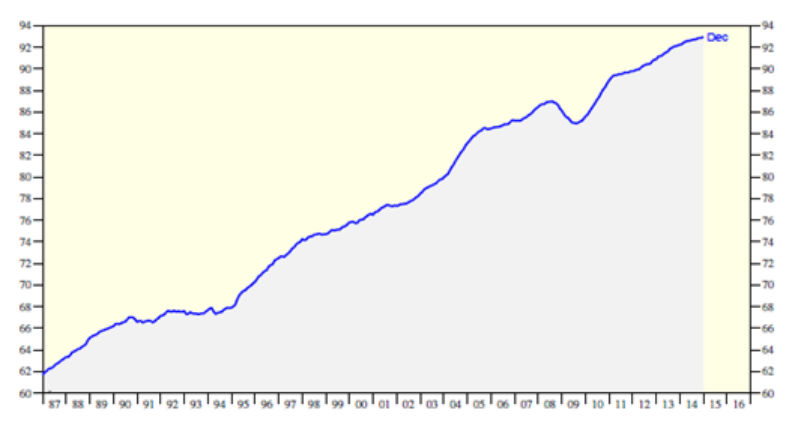
\includegraphics[width=\textwidth]{Marcteoric/Augmentdemandapetroli.png}
     	\caption{Demanda mundial de petroli, valor mig per any}
\end{figure}

\newpage

% Demanda de cotxes elèctrics al mercat
En les grans ciutats ja comencen a aparèixer polítiques que prohibeixen l'entrada a vehicles que superen un cert grau de contaminació, ja que l'acumulació d'aquest pot pujar els nivells de contaminació de la ciutat per sobre del que regeix la llei. Els vehicles elèctrics no contaminen \newline pràcticament res, si no tenim en compte el seu procés de fabricació. Els vehicles híbrids funcionen amb electricitat fins que el motor ja ha de donar una certa potència, això ja suposa que el vehicle ha d'anar a una gran velocitat, fora de les velocitats màximes permeses en una zona urbanitzada. A més a més, el preu de la gasolina és molt elevat comparat amb el de l'electricitat. 

El preu d'un vehicle de combustió o un vehicle que funciona amb electricitat no és tant distant, no estem parlant que un cotxe elèctric pugui arribar a costar el doble d'un de gasolina, els preus es troben bastant parells, tot i que encara són més econòmics els de combustió. Es preveu que per al 2022 el cost total sense subsidi per als propietaris de bateria caurà per sota de la d'un vehicle de combustió. 

Per tots aquests motius i els preus assequibles dels vehicles elèctrics, el mercat dels VE es troba en augment. La previsió per als següents anys és que la demanda creixerà de forma exponencial. Al 2040 es preveu que els vehicles elèctrics seran un 35\% de les ventes mundials d'automòbils.

\begin{figure}[H]
		\centering
    	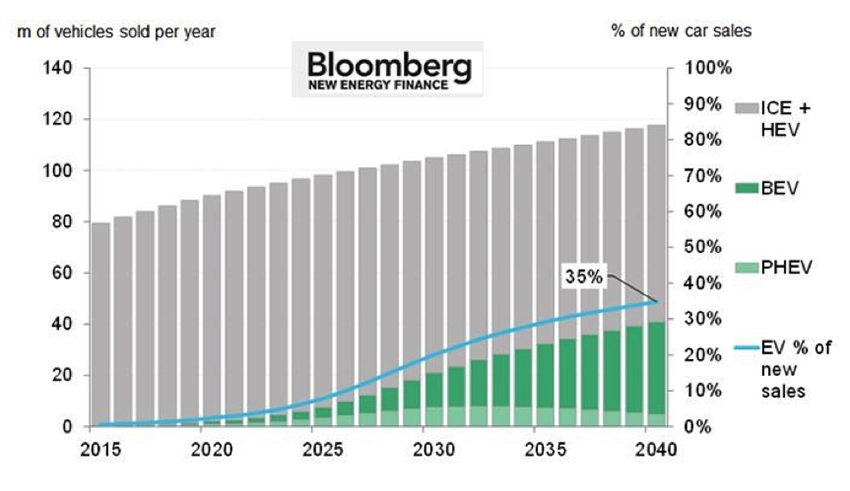
\includegraphics[width=\textwidth]{Marcteoric/ev-sales-distrib.png}
     	\caption{Previsió d'increment de la venda de vehicles elèctrics.}
\end{figure}

A la figura 2.2 es mostra de forma detallada la previsió de l'evolució del mercat dels vehicles. En primer lloc tindríem els ICE + HEV, aquests vindrien a ser els vehicles que funcionen per combustió (dièsel/gasolina) i els híbrids que també fan servir la combustió. Es pot veure com són els que lideren encara el mercat, tot indicant que el petroli seguirà sent la font d'energia principal per als vehicles en general. 

En segon lloc tindríem els BEV(Battery Electric Vehicle) que són els vehicles que funcionen mitjançant bateries. Aquests assoliran un \newline 30\% d'increment l'any 2040.Per qüestions ecològiques que podrien succeir en el futur aquest valor pot decréixer considerablement si s'estableixen límits de contaminació molt baixos. Les subvencions de l'estat per als vehicles elèctrics també podria girar la balança i que agafessin en el futur un major pes.
 

En última instància hi ha els PHEV ( Plug-In Hybrid Electric Vechicle) que són els vehicles híbrids endollables a la corrent. Encara és incert el futur d'aquest tipus de vehicles i per això no hi ha gran confiança en aquests.

\section{Mercat dels vehicles elèctrics (no cotxes)}

% Introducció
Tot i que el món dels vehicles elèctrics està totalment centrat en els cotxes, també existeixen altres vehicles que fan servir l'electricitat com a font \newline d'energia. El controlador que es plantejarà en tot aquest projecte està pensat molt més per a aquest tipus de vehicles que no pas per a cotxes. Entre aquests vehicles podríem trobar el patinet elèctric, Hoverboard i la bicicleta elèctrica entre d'altres. No només això si no que també el nostre controlador pot estar emprat per a vehicles dedicats a persones amb mobilitat reduïda com podria ser una cadira de rodes elèctrica o els típics "tricicles" que fa servir la gent gran. Per últim caldria posar els vehicles radiocontrol(RC), des de llanxes fins avions. 

Per a la majoria de vehicles esmentats no és precís aconseguir carnet de conduir o bé una llicència ni assegurança, però ve cal conèixer la normativa que regula l'ús d'aquests vehicles en llocs urbans. Cada municipi té els seus permisos i prohibicions. La normativa pot canviar depenent del pes o bé la velocitat màxima. Per això s'aconsella informar-se sobre la legislació del seu ajuntament. Sobretot a les grans ciutats és on la legislació és més estricta. Un exemple d'aquest podria ser la legislació actual de Barcelona sobre els patinets elèctrics. Els patinets elèctrics conformen els vehicles elèctrics de Tipus B.

% Normativa de patinets elèctrics a Barcelona
\begin{figure}[H]
		\centering
    	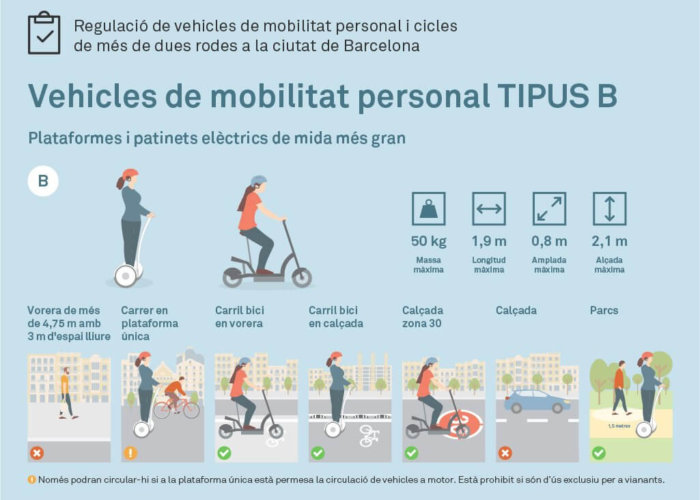
\includegraphics[width=12cm, height=7cm]{Marcteoric/normativaBCNpatinetselectrics.jpg}
    	\caption{Normativa de vehicles tipus B a Barcelona.}
\end{figure}

Si es parla de l'autonomia dels altres vehicles elèctrics no s'apropa ni de bon tros a l'autonomia d'un cotxe elèctric. Les autonomies d'aquests tipus de vehicles poden arribar als 40 minuts aproximadament, sent la bicicleta qui té una major autonomia. Depenent de la potència del motor, de la capacitat de la bateria i també com es condueixi aquest vehicle aquest temps pot variar. Un bon manteniment de la bateria també suposa una major durabilitat en l'autonomia. Ara es mostraran alguns vehicles elèctrics que són els que tenen un impacte més gran al mercat.

\subsection{Patinet elèctric}
%Patinets elèctrics
El patinet elèctric és una opció alternativa de transport ecològic per circular a nivell econòmic sense gastar res en gasolina. Són sustentables, lleugers, pràctics i ràpids. Són útils tant per aquelles persones amb mobilitat reduïda, com per estudiants, treballadors i persones amb l'objectiu de desplaçar-se d'una forma senzilla d'un lloc a un altre en un curt període de temps, estalviant gasolina i transport públic.

%Motor
L'enorme majoria dels patits tenen un motor anomenat Brush (amb escombretes de llarga durada), de gama econòmica. Els patinets elèctrics dissenyat per la conducció del peu, on el seu diàmetre de roda és més gran, disposen d'un altre gènere de motor anomenat Brushless, que vindria a fer el mateix que el motor Brush, però sense escombretes. \bigskip

%Autonomia 
L'autonomia del patinet elèctric és la combinació de múltiples factors: La capacitat de la bateria (Volts i Amperes), la potència del motor (Watts), càrrega del patinet elèctric (massa pròpia), càrrega (massa conductor), inclinació del terreny i velocitat.
En línies generals, un patinet elèctric acostuma a tenir una autonomia d'entre 40 minuts en models de 800W a 55-60 minuts en els models de 1000-1500W.
\bigskip

% Xiaomi Mi Scooter 
\subsubsection{Xiaomi Mi Scooter}  %Canviar mida per una més gran.
El Xiaomi Mi és el patinet elèctrics més venguts a la web d'Amazon. Està pensat per a una persona de fins a 75Kg. Té un abast de fins a 30Km amb una sola càrrega. Pot arribar a velocitats de fins a 35Km/h. El seu preu ronda els 380€. 
\begin{figure}[H]
		\centering
    	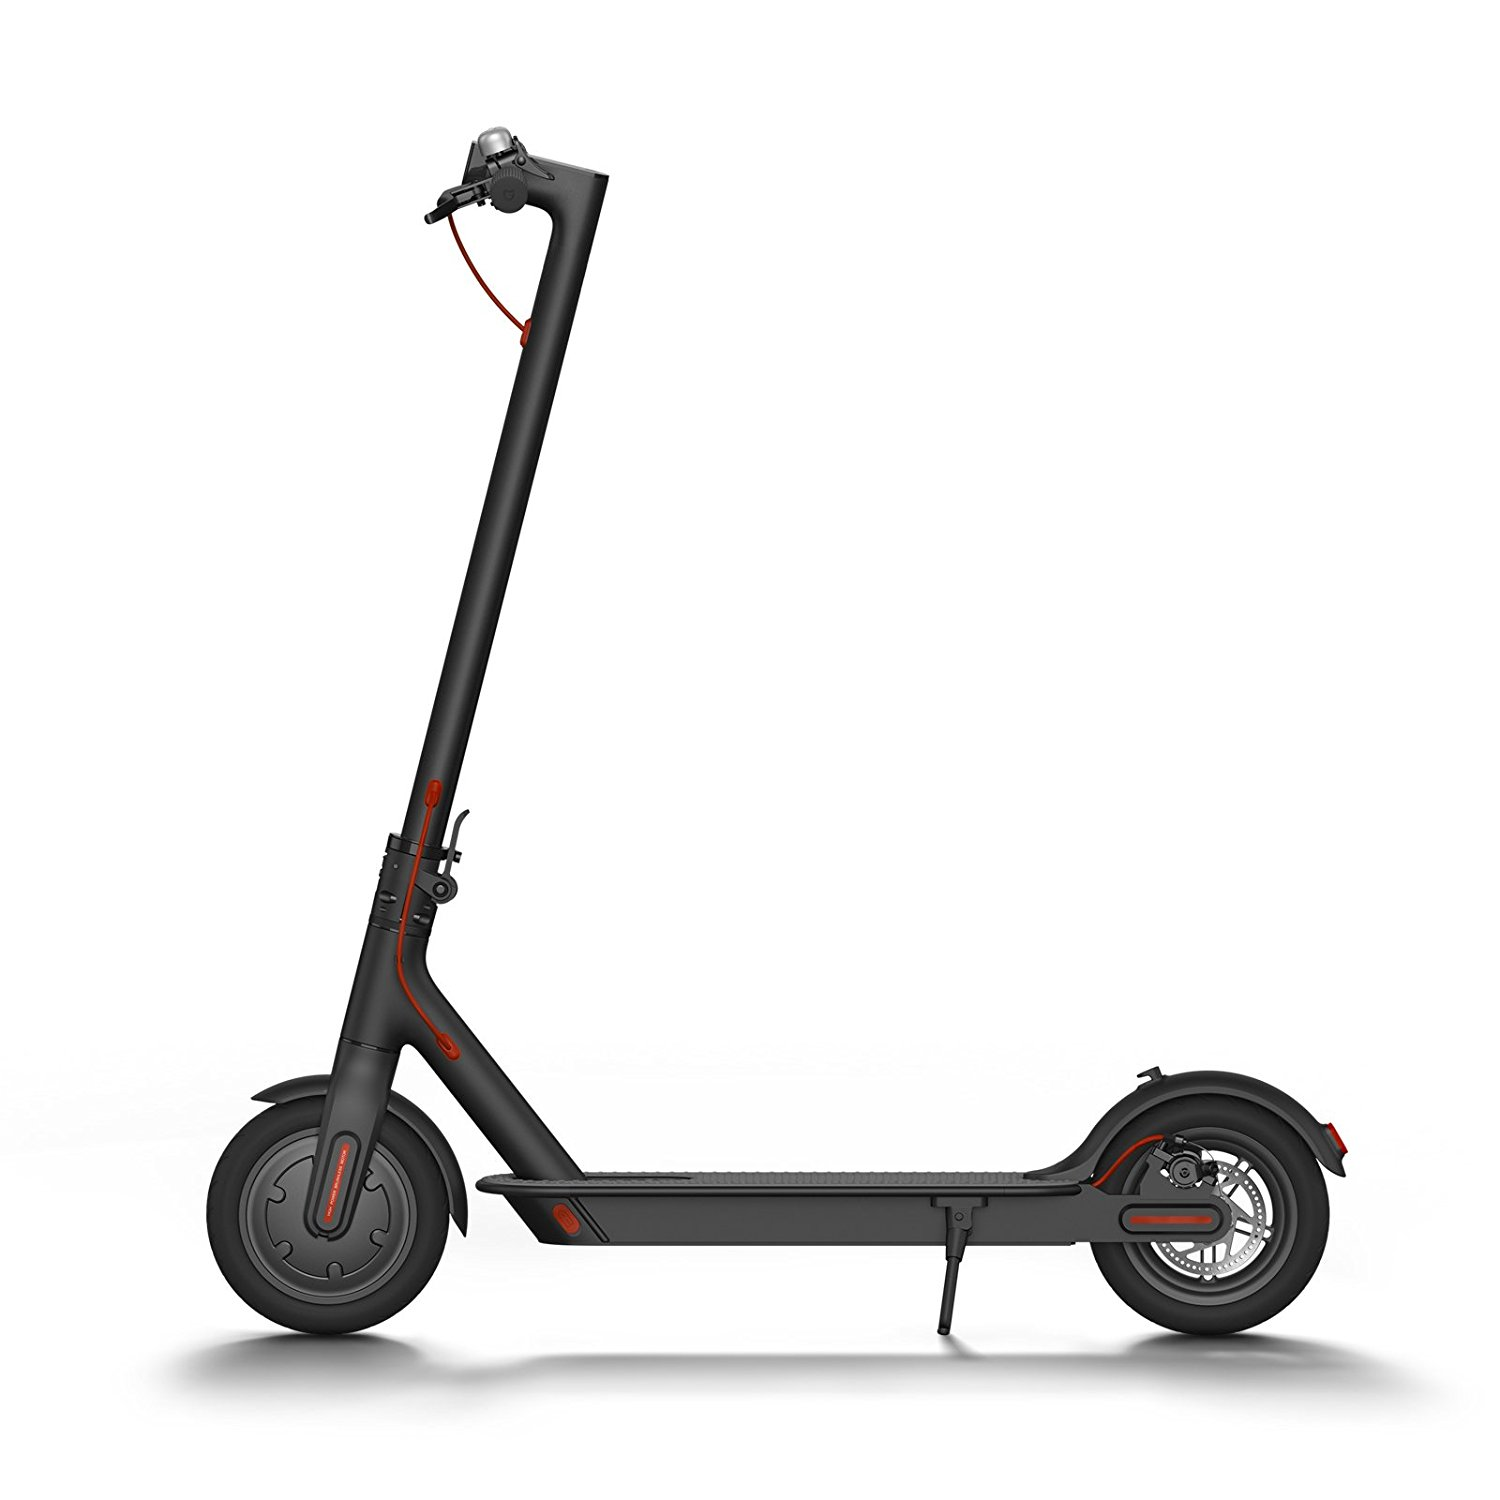
\includegraphics[width=10cm, height=10cm]{Marcteoric/patinetelectricxiamoi.jpg}
     	\caption{Xiaomi Mi Scooter.}
\end{figure}

\newpage

%Homcom Patinet elèctric
\textbf{Homcom Patinet elèctric} \bigskip \newline %Canviar per una mida més gran
El Homcom és un patinet plegable elèctric tipus Scooter, aquest model es trobaria a la gama baixa de patinets elèctrics. Està pensat per a una persona de fins a 50Kg. Té un abast d'entre 10-15Km amb una càrrega sencera. Pot arribar a una velocitat de fins a 12Km/h. El seu preu ronda els 100€.
\begin{figure}[H]
		\centering
    	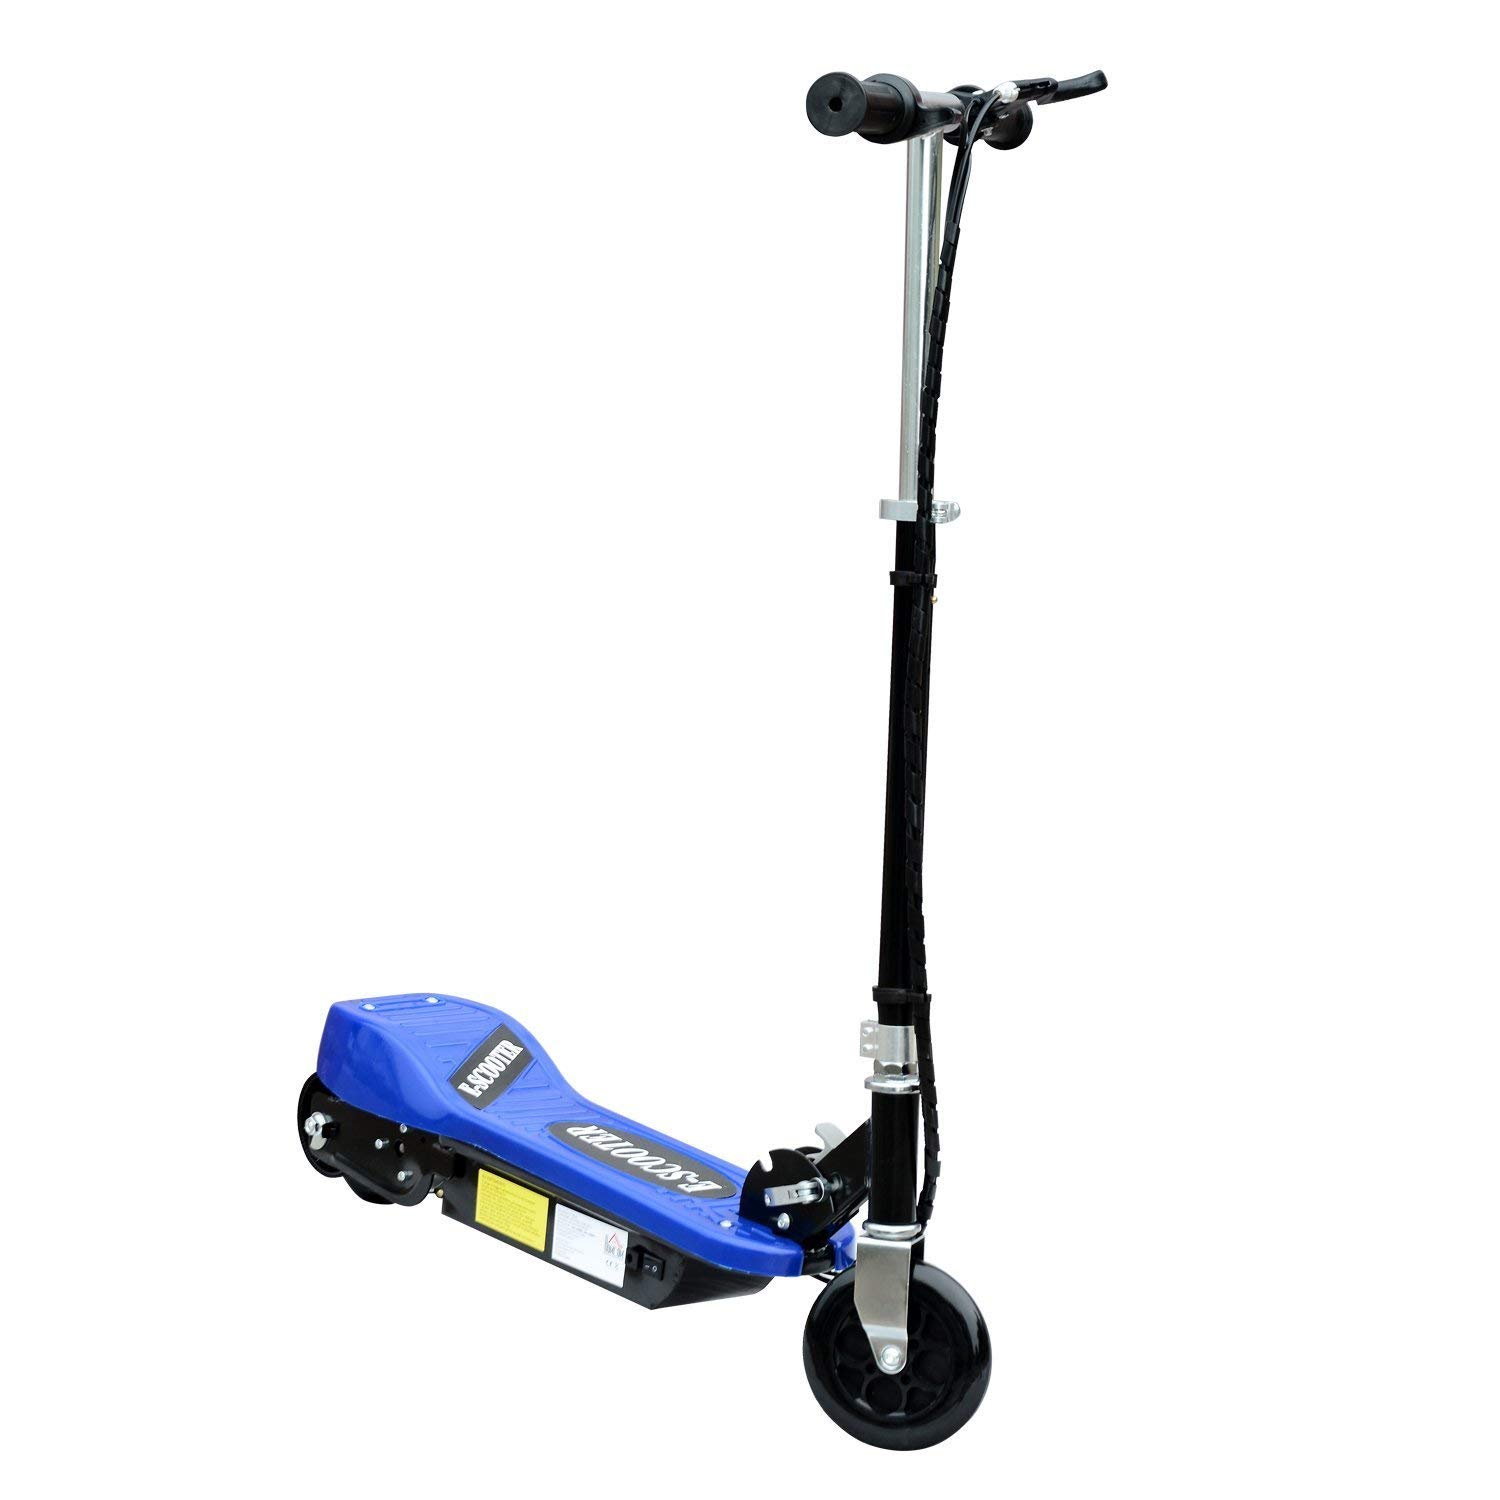
\includegraphics[width=8cm, height=8cm]{Marcteoric/Homcompatinetelectric.jpg}
     	\caption{Homcom patinet elèctric}
\end{figure}

%Hoverboard

\subsection{Hoverboard}
Aquests patinets han aparegut fa poc temps. Són únics en la forma en la que funcionen ja que s'autoequilibren, de tal forma que l'usuari pot accelerar i frenar tan sols movent el seu cos cap endavant o cap enrere. De la mateixa manera, girar és tan senzill com inclinar lleugerament el cos cap a un costat o l'altre. El funcionament d'aquest patinet es basa en el funcionament de diferents mecanismes. En primer lloc, les bateries es connecten a dos motors elèctrics independents en cada roda. Per altra banda, es troba el component més important per a mantenir l'equilibri, el giroscopi. Aquest detecta quan canvia d'orientació el patinet per a, d'aquesta forma, poder mantenir l'orientació adequada. 

El giroscopi funciona mitjançant un sensor magnètic que detecta la direcció de moviment i la velocitat rotacional de la roda. 
Tot el sistema es troba connectat a una unitat central de processament (CPU). El giroscopi mesura constantment l'orientació de la roda, i envia un senyal a la CPU per a que es processi e interpreti. D'aquesta forma, si el patinet s'inclina cap endavant s'envia l'ordre d'accelerar els motors per a compensar aquesta inclinació. Pel contrari, si s'inclina cap enrere es produirà l'efecte invers. Ara es mostraran dos exemples per veure com estan implantats aquests productes al mercat. \newline \bigskip

%Hooboard
\textbf{Hooboard} \bigskip \newline  
El Hooboard és un Hoverboard de gama alta. Té una autonomia de fins a 15Km i una velocitat màxima de fins a 15Km/h. Està composat per dos motors de 400W i el seu preu ronda els 500€.
\begin{figure}[H]
		\centering
    	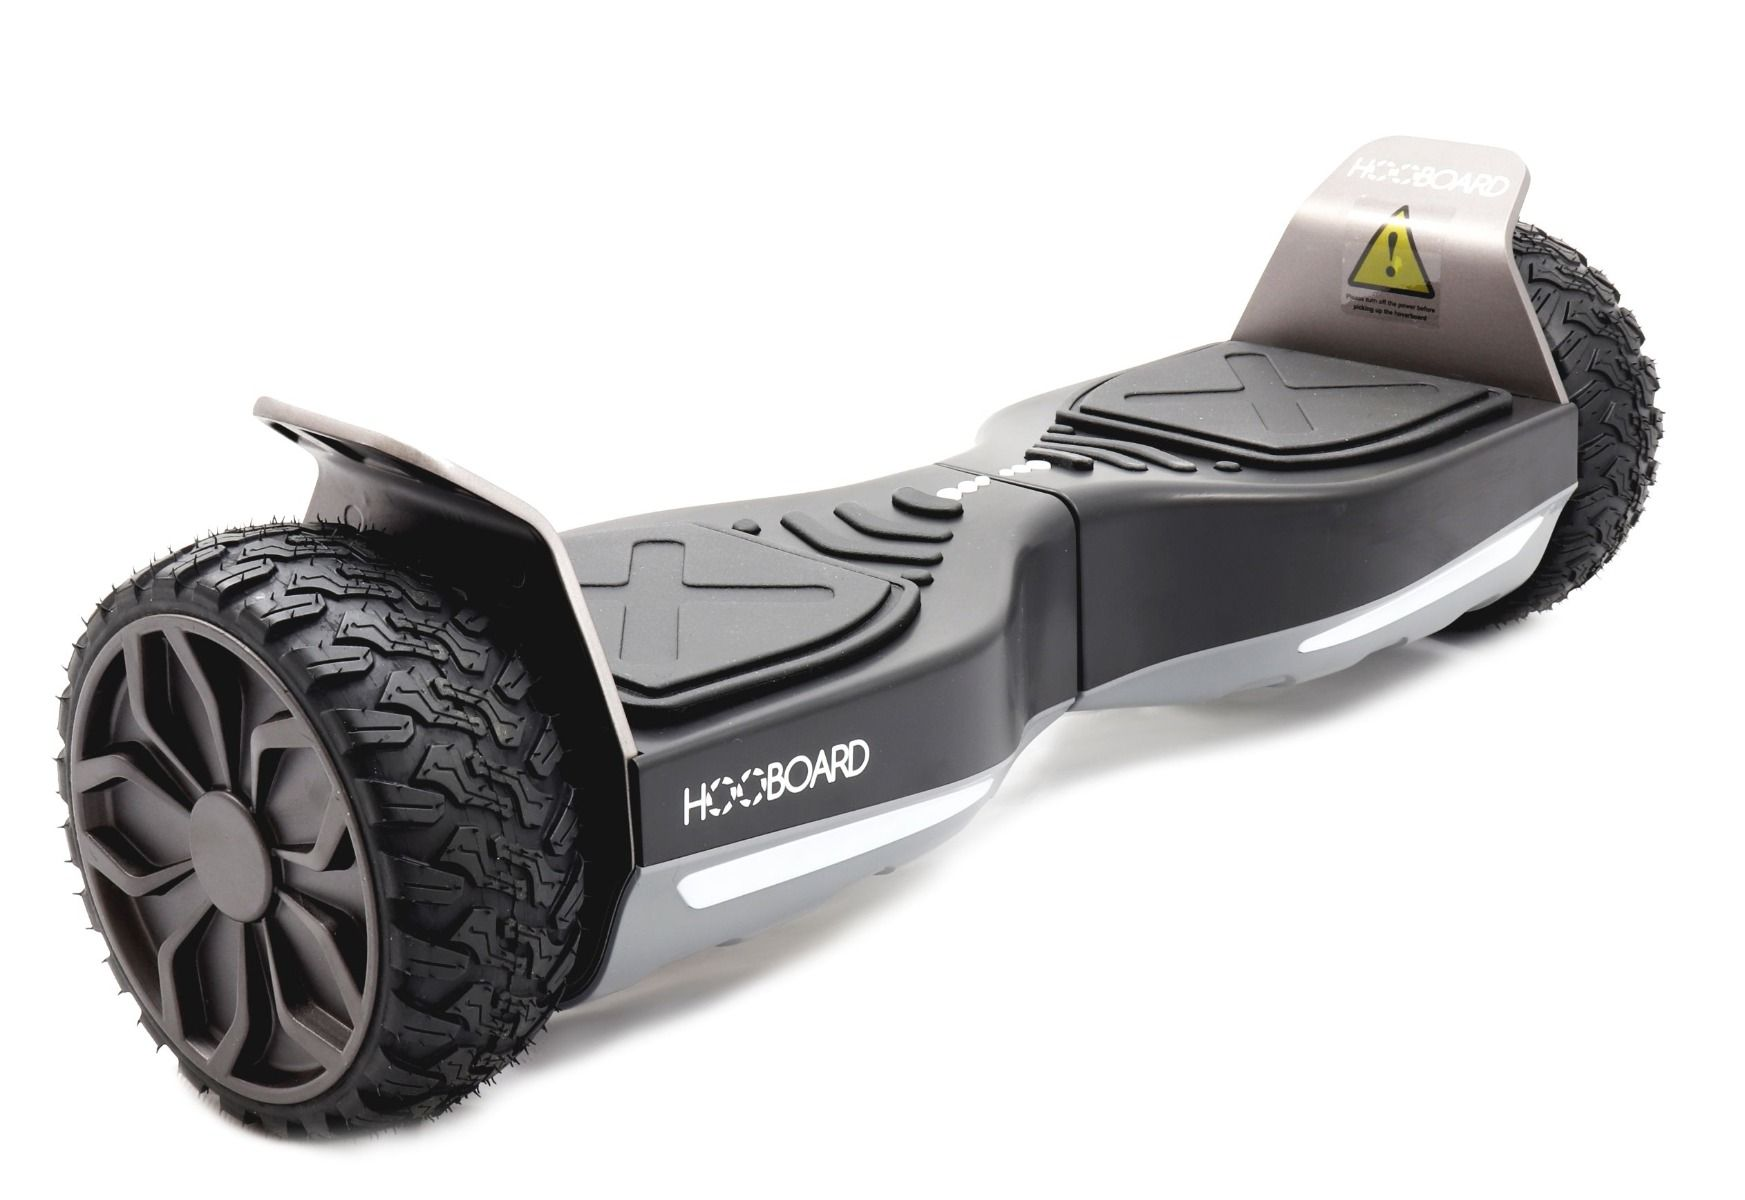
\includegraphics[width=9cm, height=7cm]{Marcteoric/hooboard.jpg}
     	\caption{Hooboard}
\end{figure}

\newpage

% BEBK Hooverboard
\textbf{BEBK Hooverboard} \bigskip  \newline % canviar per una mida més gran
El BEBK Hooverboard és un Hooverboard que funciona mitjançant motors elèctrics Brushless. Consta de dos motors de 350W. Pot arribar a velocitats de fins a 12Km/h i una autonomia de fins a 18Km. El seu preu ronda els 150€.
\begin{figure}[H]
		\centering
    	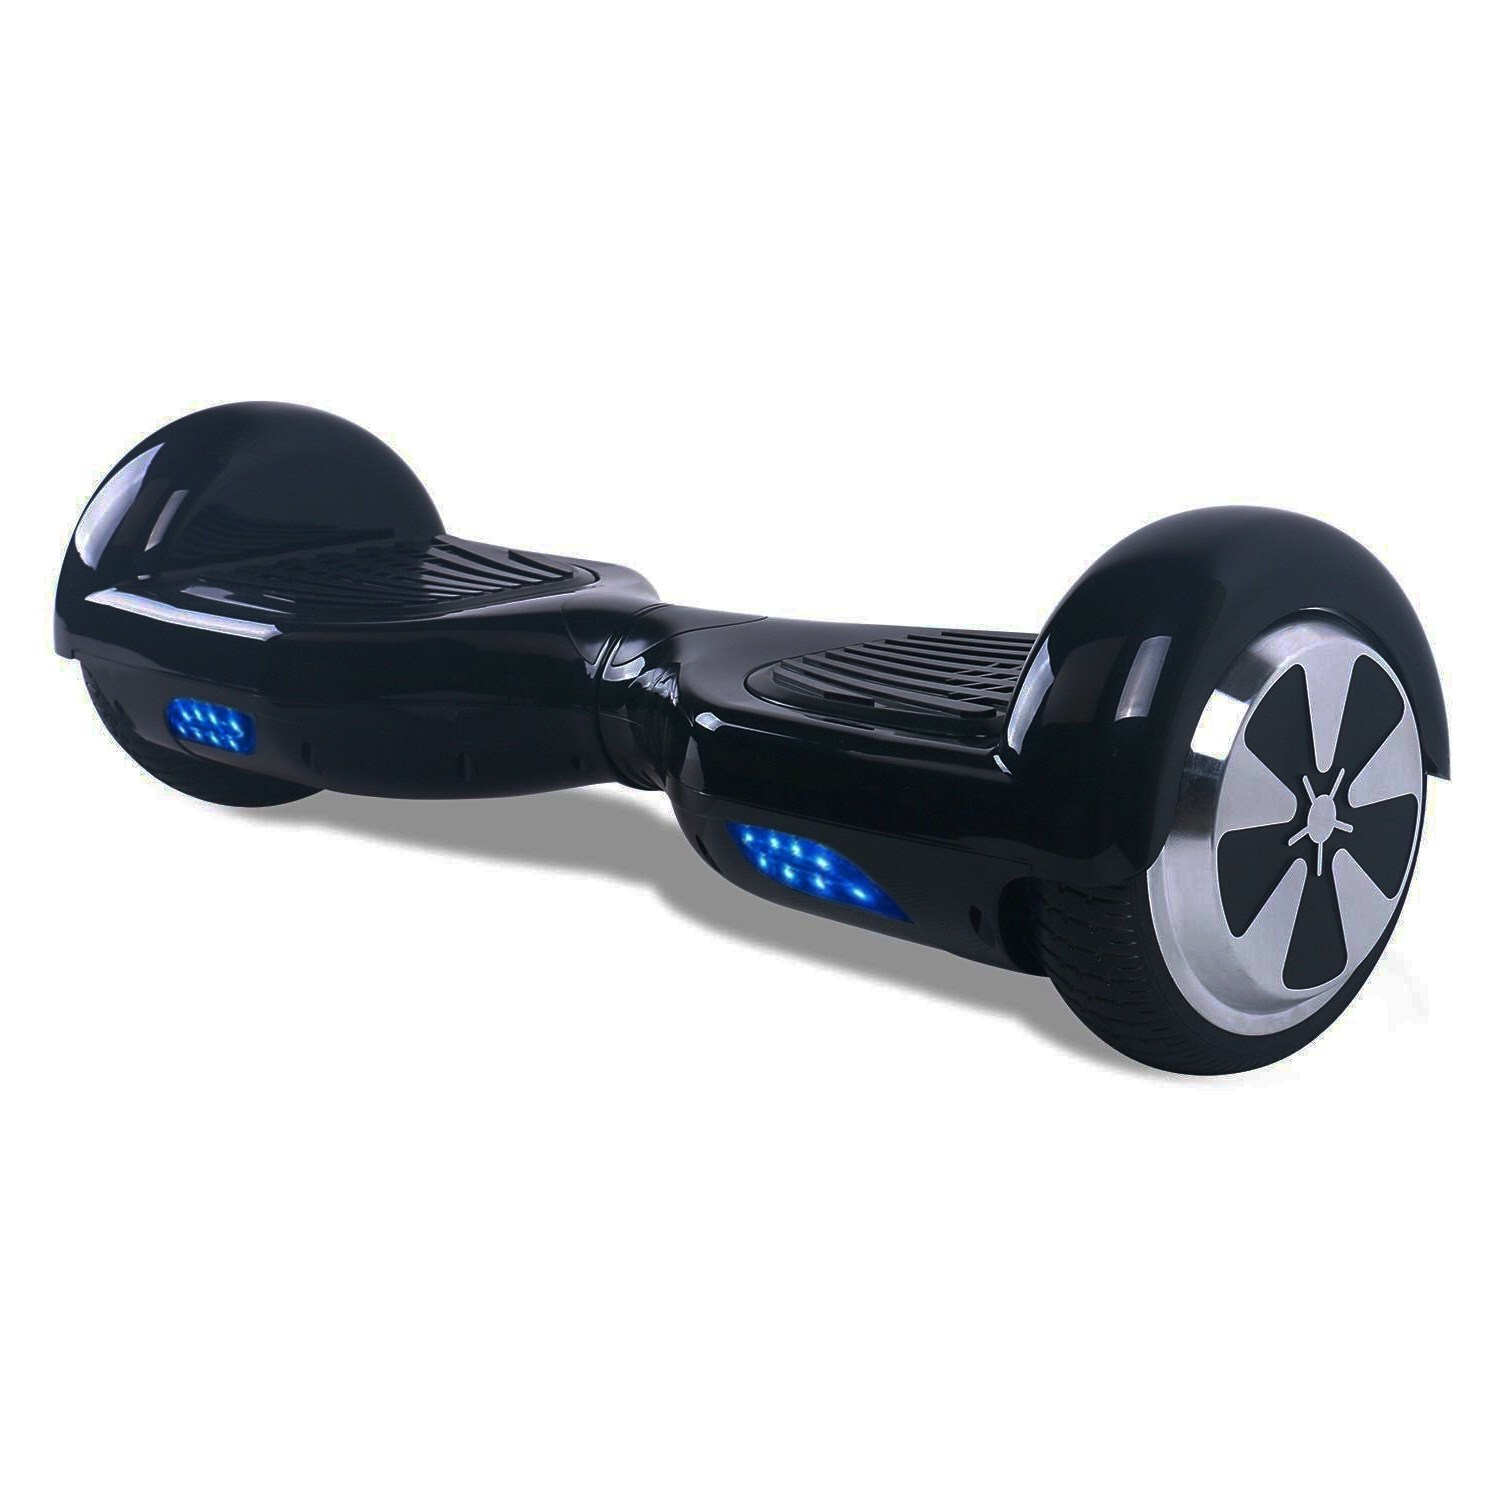
\includegraphics[width=7cm, height=7cm]{Marcteoric/bebkhooverboard.jpg}
     	\caption{BEBK Hooverboard}
\end{figure}

\subsection{Bicicleta elèctrica}
% Bicicletes elèctriques
Al 2016 les ventes de bicicletes elèctriques van arribar, en tot el món, a uns 35 milions d'unitats. La millora de la tecnologia de les bateries d'ions de liti està donant com a conseqüència bicicletes elèctriques més lleugeres, més econòmiques i cada cop més similars a les bicicletes tradicionals.

Les altes tasses d'urbanització, la millor de la tecnologia de les bateries i els components de les bicicletes, les polítiques locals relacionades amb la contaminació, el desig creixent d'abandonar modes de transport motoritzats, el seu major rendiment i baix cost impulsen la indústria de la bicicleta elèctrica. Les bicicletes elèctriques es troben situades en una posició ideal per a ser les majors beneficiades d'aquesta tendència de canvi, pel seu baix cost en relació amb l'automòbil, per no requerir carnet pel seu maneig i per l'existència, cada cop en major mesura d'infraestructures especialment dedicades a elles. \newline \bigskip

% Extrbici XF800 Electric ATV                 
\textbf{Extrbici XF800 Electric ATV } \bigskip	\newline	% canviar per una mida més gran
L'Extrbici XF800 Electric ATV és una bicicleta elèctrica que pot portar una càrrega de fins a 160Kg, pot arribar a 50Km/h amb una autonomia relativa de fins a 80Km. El seu preu rondaria els 1900€
\begin{figure}[H]
		\centering
    	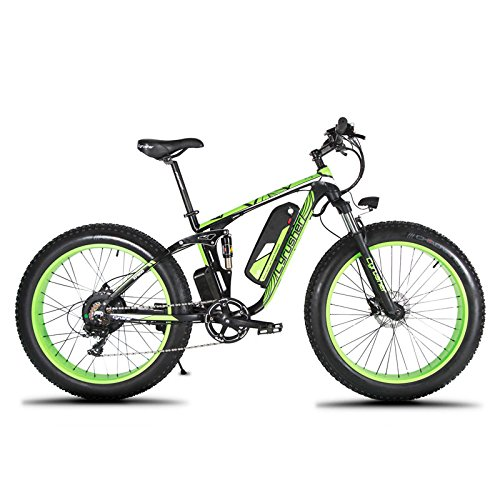
\includegraphics[width=10cm, height=10cm]{Marcteoric/extrbicixf800electricatv.jpg}
     	\caption{Extrbici XF800 Electric ATV}
\end{figure}
% FOLLOW UP E05                        
\textbf{FOLLOW UP E05 }	\bigskip \newline			% canviar per una mida més gran
El FOLLOW UP E05 és una bicicleta elèctrica que pot portar una càrrega de fins a 100Kg, pot arribar a 22Km/h amb una autonomia de fins a 30Km. Funciona amb motor Brushless de 250W i el seu preu ronda els 400€.
\begin{figure}[H]
		\centering
    	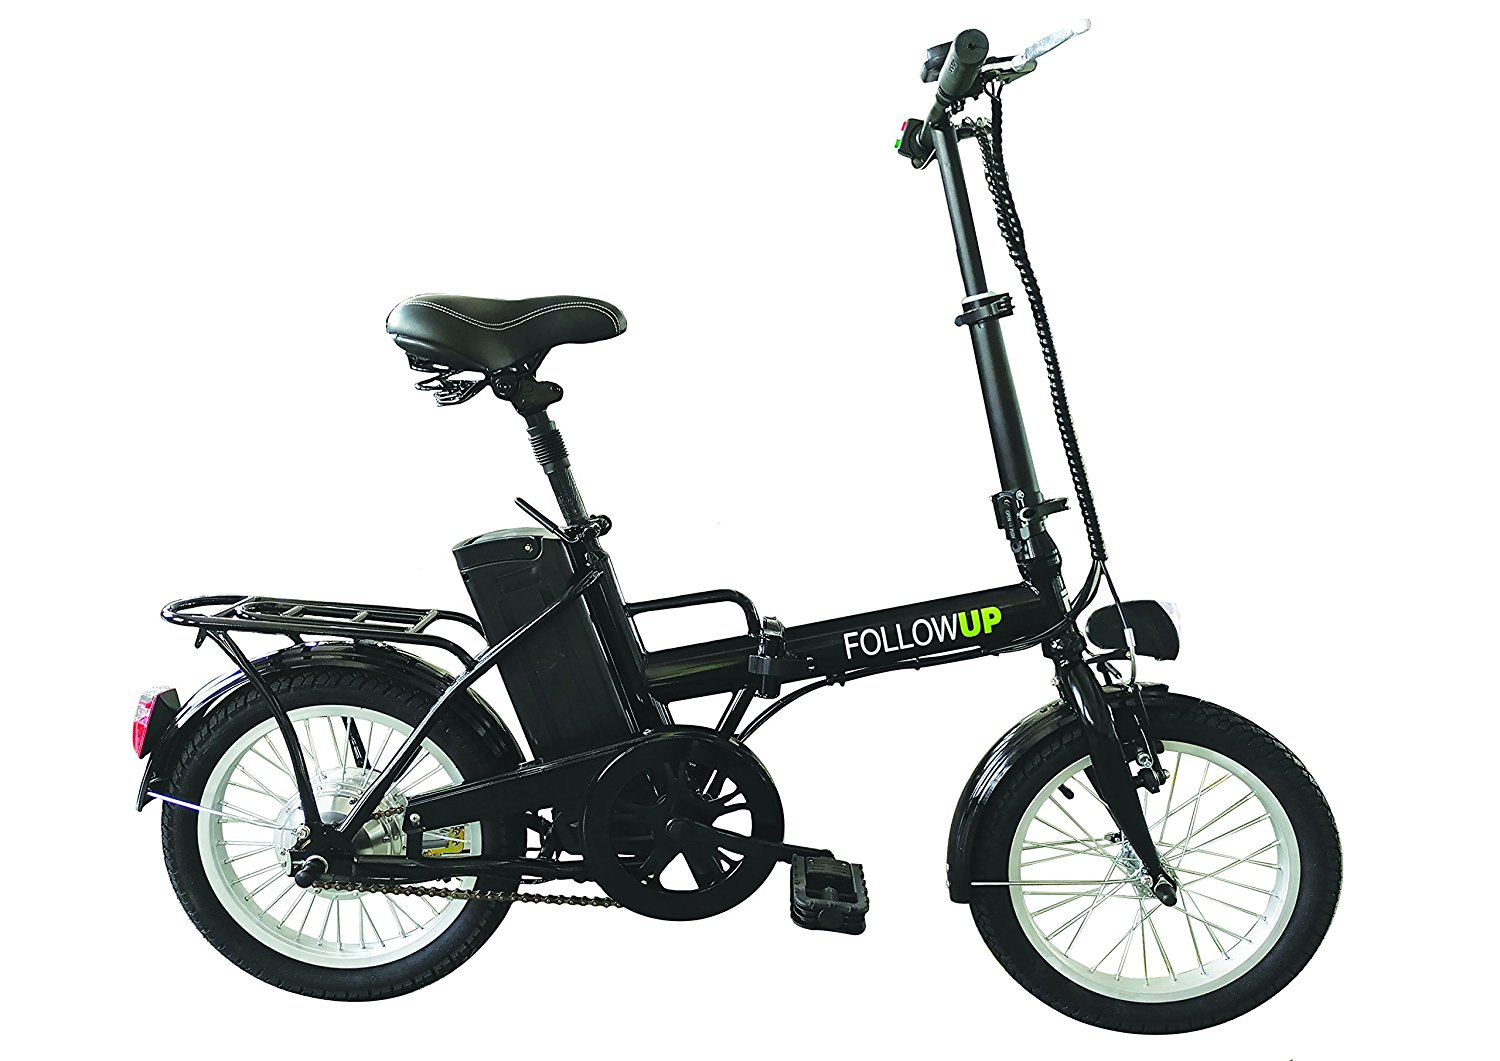
\includegraphics[width=10cm, height=7cm]{Marcteoric/followupe05.jpg}
     	\caption{Extrbici XF800 Electric ATV}
\end{figure}

%!!!!!!!!!!!!!!!!!!!!!!!!!!!!!!!!!!!!!!!!!!!!!!!!!!!!!!!!!!!!!!!!!!!!!!!!!!!!!!!!!!!!!!!!!!!!!!!!!!!!!!!!!!!!!!!!!!!!!!!!!!!!!!!!!!!!!!!!!!!!!!!!!!!!!!!!!!!!!!!!!!!!!!!!!!
% Conclusió total
%Aquests vehicles suposaran la facilitat de desplaçar-se d'una forma ràpida i còmode, ja que l'electricitat de la bateria serà qui s'encarregui de la transports ràpids no contaminants on les persones podran desplaçar-se 
%!!!!!!!!!!!!!!!!!!!!!!!!!!!!!!!!!!!!!!!!!!!!!!!!!!!!!!!!!!!!!!!!!!!!!!!!!!!!!!!!!!!!!!!!!!!!!!!!!!!!!!!!!!!!!!!!!!!!!!!!!!!!!!!!!!!!!!!!!!!!!!!!!!!!!!!!!!!!!!!!!!!!!!!!!!

\section {Mercat de les bateries emprades per als VE}

%Introducció
Les bateries d'ió-liti ja formen part de la vida quotidiana i estan incloses en telèfons mòbils, tauletes i raspalls de dents elèctrics, entre d'altres aplicacions. En els últims anys s'han produït diferents avenços tecnològics en aquest tipus de bateries per a poder ser emprades en els vehicles elèctrics. Encara que l'adopció dels vehicles elèctrics no estigui sent tan positiva com s'esperava, les bateries ja suposen un component cada cop més rellevant dins de la indústria automobilística. Donat que les bateries són una part significativa dels costos d'un vehicle elèctric, existeixen considerables incentius per augmentar l'eficiència dels seus processos de producció, reduir els seus costos i millorar el seu rendiment. El sistema elèctric es beneficiarà del desenvolupament d'aquestes bateries, al construir una solució per emmagatzemament de l'energia generada per les tecnologies renovables intermitents, que permetran reforçar la seva seguretat de subministrament.

Respecte als reptes que té aquesta tecnologia a superar, cal destacar la falta d'una única tecnologia d'emmagatzemament que sigui capaç de cobrir totes les necessitats del mercat. Això provocarà que el sistema pugui contemplar la incorporació de diferents tipus de bateries. 

\newpage 

Addicionalment, a l'igual que qualsevol altre component del sistema elèc- \newline tric, els sistemes de gestió de bateries hauran de lidiar amb els possibles atacs tecnològics que puguin sofrir. En definitiva, el desenvolupament dels vehicles elèctrics permetrà avançar en les tecnologies de bateries \newline d'emmagatzemament. Les bateries hauran de considerar-se com a part de l'estratègia de les energies renovables, contribuint a arribar a un sistema energètic més eficient.

\subsection{Previsió de mercat per al futur de les bateries}

Com ja s'ha comentat prèviament, les bateries jugaran un paper molt important dintre dels vehicles elèctrics. Això vol dir que ja s'implementen estratègies per tal d'optimitzar el màxim els costos i rendiment d'aquestes. A la dècada del 2030 podríem estar parlant que el preu de baixada respecte el 2010, que és quan van començar a aparèixer de forma global les bateries d'ió-liti estaria suposant aproximadament una reducció de cost de fins al 75\%. No només es reduiran els preus de les bateries, sinó que la compra \newline d'aquestes bateries augmentarà considerablement en els últims anys arribant a valors que superin els catorze mil milions de dòlars l'any 2026.
\begin{figure}[H]
		\centering
    	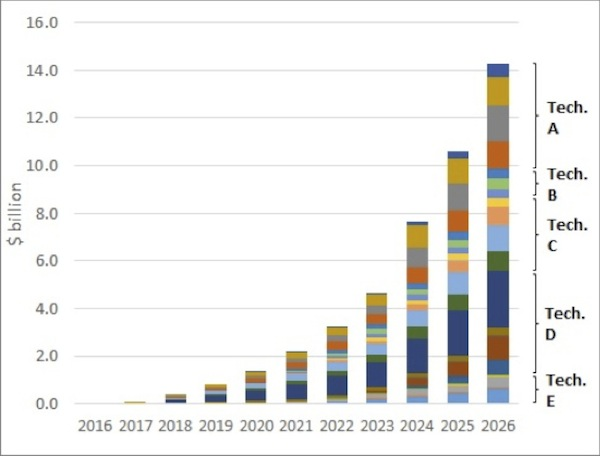
\includegraphics[width=13cm, height=8cm]{Marcteoric/ventabateries2026.jpg}
     	\caption{Previsió de ventes de bateries en funció del tipus de vehicle} 
\end{figure}

\subsection{L'hora de l'economia del liti}
Les bateries de liti estan totalment consolidades a la vida quotidiana. Són necessàries per alimentar des de petits dispositius fins a sofisticats vehicles elèctrics. La previsió és que el seu consum augmenti en els pròxims anys, especialment fomentat per l'auge de l'Internet de les Coses i altres aplicacions tecnològiques.

Degut a la predicció del decreixement del cost d'aquest tipus de bateries s'està impulsant de forma massiva aquest mercat. Aquesta caiguda de preus és probable que provingui d'un augment de la demanda degut a la propagació dels cotxes elèctrics, que està permetent als fabricants augmentar la producció. 
\begin{figure}[H]
		\centering
    	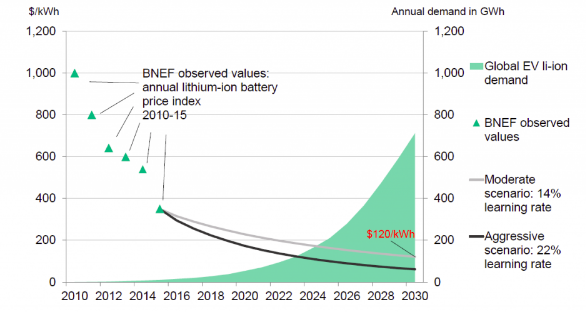
\includegraphics[width=13cm, height=8cm]{Marcteoric/mercatbaterialitioion.png}
     	\caption{Previsió del mercat de les bateries d'ions del liti.} 
\end{figure}

\subsection{Drivers de motors elèctrics}
% Drivers
%		Introducció
% 		Turnigy Dlux 250A 60V HV 14s ESC
% 		VESC 6 Complete - Vedder Electronic Speed Controller TRAMPA Exclusive
% 		Turnigy SK8-EXC V4.12 For Electric Skateboard Conversion w/BEC
% 		Controlador d'alta potència (Per buscar)	% DE MOMENT AQUEST L'IGNORO

% Introducció
Un sistema de control o controlador per a un motor elèctric podria definir-se com un dispositiu conjunt al motor, que serveix per governar d'alguna manera predeterminada l'operació del motor i que a més a més proporciona algun tipus de protecció que asseguri el seu funcionament. Els controladors poden ser molt senzills o extremadament complexes.\bigskip

avi en dia el motors predominats son els bruslles tan per aplkicacionde de hobby com veicels rc coma pets i mitgans veicles electris, per tan comentarem alguns dirnvers del marcat per tal de governar aquets motors per esmatar les sevas caracteristas i tenir una idea de quines magnituts es mouen els seus valors 
% !!!!!!!!!!!!!!!! AFEGIR ALGUNES COSETES MES COM A INTRODUCCIÓ?

\textbf{Turnigy Dlux 250A 60V HV 14s ESC}\bigskip \newline  
%Introducció del producte
Aquest ESC fa servir un disseny de PCB doble que separa l'alimentació del motor i del microcontrolador. Aquest disseny permet la disposició dels components òptims en cada PCB i proporciona la configuració ideal per la dissipació de calor i l'eficiència tèrmica. Ambdues PCB estan tancades en una carcassa d'alumini dissipador de calor per assegurar la dispersió de calor màxima. Las Fet de commutació en aquest CES són genuïnes de qualitat superior. El seu preu està al voltant dels 188€.
Tots els CES Turnigy Dlux es poden programar a través d'una tarjeta de programació o pel transmissor. \newline \bigskip 
% Especificacions
Especificacions:
	\begin{itemize}
            \item Intensitat continua màxima: 250A
            \item Max Burst actual: 275A
            \item BEC: N / A (OPTO)
            \item Lipo: 6 - 14S
            \item NiMH: 18 - 42 cel·les
            \item Pes: 456 grams
            \item RPM Max (2 pols): 200.000 rpm
            \item Mida: 135x77x50 mm
	\end{itemize}
% Característiques
Característiques:
	\begin{itemize}
			\item Baixa resistència interna
			\item Baixa temperatura de funcionament
			\item Protecció de sobreescalfament
			\item Eliminador d'espurnes
			\item Hexfets alta qualitat (MOSFETs)
	\end{itemize}
%Imatge
\begin{figure}[H]
		\centering
   	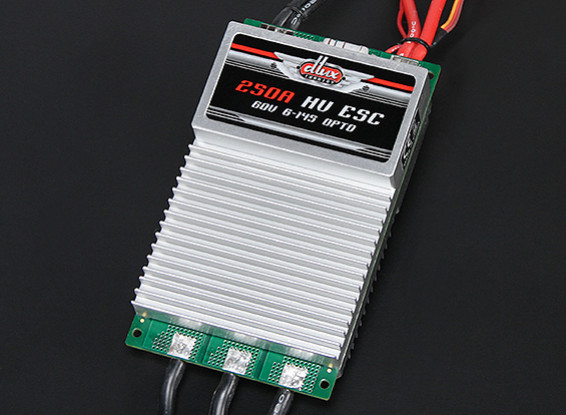
\includegraphics[width=8cm, height=8cm]{Marcteoric/250Hobydriver.jpg}
     	\caption{Turnigy Dlux 250A HV 14s ESC} 
\end{figure}
%Conclusions del producte        !!!!!!!!!!!!!!!A REVISAR
%Són controladors originalment dissenyats per controlar aparells RC, la seva potència pot perfectament ser emprada per a petits vehicles elèctrics. Dóna perfectament per moure patinets o bicicletes elèctriques. Funciona a 60V, per tant el voltatge de la bateria no seria molt perillós a l'hora de treballar-hi. Però li faltarien algunes funcions important com la frenada regenerativa i alguns controls d'arrencada progressiva i frenada que farien que l'autonomia i la comoditat de la conducció augmentés moltíssim. \bigskip

% VESC 6 Complete - Vedder Electronic Speed Controller TRAMPA Exclusive
% 		Introducció del producte	Per fer
% 		Especificacions				OK
% 		Característiques			OK
%		Imatge						OK
% 		Conclusions del producte	Per fer
\textbf{VESC 6 Complete - Vedder Electronic Speed Controller TRAMPA Exclusive}\smallskip
% Introducció del producte
 %!!!!!!!!!!!!!!!!!!!!!!!!!!!!!!!!!!!!!!!!!!!!!!!!!! PER FER
%\newline \bigskip 
% Especificacions
Especificacions:
\begin{itemize}
	\item Voltatge: 6V-60V (Segur per a 3S fins a 12S LiPO).
	\item Corrent: Continua 80A. Burst 120A. 
	\item 5V 1A de sortida per a electrònica externa.
	\item 3.3V 0.5A de sortida per a electrònica externa.
	\item Modes: DC, BLDC, FOC (sinusoïdal)
\end{itemize} 
% Característiques
Característiques:
\begin{itemize}
	\item Mesura de corrent i voltatge en totes les fases
	\item Frenada regenerativa
	\item Control de tracció (Simple i Parell)
	\item Sensored or Sensorless Operació + Mode híbrid
	\item Ports de comunicació: USB, CAN, UART
	\item Protecció ajustable per a definir els límits màxims i mínims \newline del voltatge i la corrent
\end{itemize}
% Imatge
\begin{figure}[H]
	\centering
	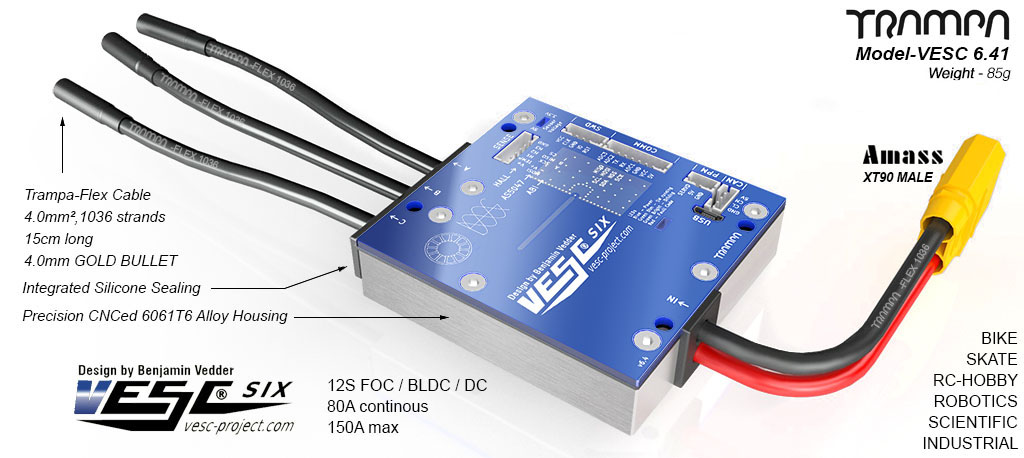
\includegraphics[width=\textwidth, height=8cm]{Marcteoric/drivertrampavesc6.jpg}
 	\caption{Turnigy Dlux 250A HV 14s ESC} 
\end{figure}

% Conclusions del producte
%!!!!!!!!!!!!!!!!!!!!!!!!!!!!!!!!! PER FER


% Turnigy SK8-EXC V4.12 For Electric Skateboard Conversion w/BEC
% 		Introducció del producte	Per fer
% 		Especificacions				OK
% 		Característiques			OK
%		Imatge						Per posar
% 		Conclusions del producte    Per fer

\textbf{Turnigy SK8-EXC V4.12 For Electric Skateboard Conversion w/BEC}

% Introducció del producte

% Especificacions
Especificacions: 	
\begin{itemize}
    \item Amperatge : 120A continu / 240A pic: 50A continu / 24            
	\item Cel·les: LiPo 3-12S
    \item Voltatge: 12.6 - 60V
    \item BEC 5V@1.5A
    \item Tipus BEC: Suport intern del controlador
    \item Timing: Calibratge Software
    \item Freqüència: PWM input
    \item Pes: 80gr
	\item Mides: 60x40x20mm
\end{itemize}

% Característiques
Característiques:
\begin{itemize}
	\item Frenada Regenerativa
	\item Sensored and Sensorless (FOC) permet que l'skate elèctric funcioni sense fer soroll el motor
	\item Seguretat: Control actual, funcions de control de temperatura
	\item Bona arrencada amb motors sensorless.
	\item Connectors de bala 12awg amb connector de bala de  4mm
\end{itemize}

% Conclusions del producte
%aqui etem parlant de dos controladors derivats del VESC un es una versio produda per sk8 del progecta obert o el vesc6 que es una versio millorada per una empresa privada derivan del que sera explicat mes endavent, tenan un sistema de aracada mes soua rampas i controlas de la frenada regenrativa i fan que la expariencia de conducio sigui mes amigable i eficas que amb un controlador de hoby 

%!!!!!!!!!!!!!!!!!!!!!!!!!!!!!!!!!!!!!!!!!!!!!!!!!!  DE MOMENT AQUEST L'IGNORO
% Controlador d'alta potència (Per buscar)
% 		Introducció del producte
% 		Especificacions
% 		Característiques
%		Preu
% 		Conclusions del producte

%\textbf{controladors comercial de alta potecia}\smallskip

% Introducció del producte
%http://www.sevcon.com/products/high-voltage-controllers/

% Especificacions
%Up to 800V DC peak supply voltage
%Up to 300kW peak power output
%Up to 150kW continuous power output

% Característiques

% Preu

% Conclusions del producte
%tambe tindriam una gama de controladors profecianls com el sevcon gen4-s10 que es un controlador disenyat per portar motors electrics desde  800V amb potencias de 150KW continus i pics de 300kw, tenen comunicacions amb can open per poder extreure o intruidir dadedes i els parametres de configuracio per tal de ferlos comportar com a EV o controladors indistrials. 


%!!!!!!!!!!!!!!!!!!!!!!!!!!!!!!!!!!!!!!!!!!!!!!!!!!!!!!!!!!!!!!!!!!!!!!!!!!!!!!!!!!!!!!!!!!!
% CONCLUSIONS TOTALS ?
%!!!!!!!!!!!!!!!!!!!!!!!!!!!!!!!!!!!!!!!!!!!!!!!!!!!!!!!!!!!!!!!!!!!!!!!!!!!!!!!!!!!!!!!!!!!

\section{Recerca de projectes de controladors de vehicles elèctrics de codi obert}
% BRUNET: POSA ALMENYS ELS LINKS DE POSSIBLES CONTROLADORS QUE PODRIEM COMPRAR AL MERCAT, ALMENYS NECESSITARIA UN PARELL D'ELLS, EL MODEL ECONOMIC I EL MODEL TOP DE GAMA. POSANT-ME EL LINK DEL PRODUCTE JA EM PODRIA ENCARREGAR JO D'OMPLIR TOT
% EVOLUCIÓ DEL MERCAT DELS CONTROLADORS
% EVOLUCIÓ DE LES TECNOLOGIES DELS CONTROLADORS EN UN FUTUR
% PACK TODO EN UNO
% DOS PACKS: BMS Y VESC


en al marcat actual tenin diversos controladors disponibles desde controlador de veicles de hoby i com coches o barcos RC fins a intermitgos i dedicats a pettis ev. tot tells tenan unas ventags i incovaniments derivats de la aplicacio en cuestio per que estan densenyats. esmatem les sevas caractaristiques: \bigskip

\textbf{HOBY:}\smallskip

son controladors original ment disenyats per controlar aparells de rc pero que la seva potecia pot perfectament ser utilisats en petits EV \smallskip

amb una potenica maximas de alguns models de 16.170w dona perfectament per poder moure patinets o bicicletes elecricas, el seu voltage baix 60 V  mes o menos, no seria molt parillos en estar en voltages vaixos, tenen el inconvaient que trevallan a gran intencitats i axo probo problemas se soroll i emis que san de tenir en conte tamde li faltan algunes funcions inportant com la frenada regenerativa i alguns control de arecada perogesia i frenada que farien que la autonima i la comoditat de cundocio aumantes moltisim. %\bigskip


\textbf{disaney per ev:}\smallskip

son controladors com alguns mdodels se sevcon o vesc entre molts altres, tenen potencias mes altesn el algun cas apar trevallaon a voltges molt mes alts, en el cuals san de tenir en conte, axo perment reduir la intenciat i disminir la secio del cables, disposne de control de frenada regentiva tan per rgenrar potencia o per cremar aquesta corrent contorl del ciquit de potencia

\textbf{controladors comercial de alta potecia}\smallskip

http://www.sevcon.com/products/high-voltage-controllers/

Up to 800V DC peak supply voltage
Up to 300kW peak power output
Up to 150kW continuous power output

tambe tindriam una gama de controladors profecianls com el sevcon gen4-s10 que es un controlador disenyat per portar motors electrics desde  800V amb potencias de 150KW continus i pics de 300kw, tenen comunicacions amb can open per poder extreure o intruidir dadedes i els parametres de configuracio per tal de ferlos comportar com a EV o controladors indistrials. 

% BRUNET: POSAR ALMENYS ELS LINKS DE POSSIBLES PROJECTES QUE PODRIEM TINDRE EN COMPTE PER A LA REALITZACIO DEL NOSTRE PROJECTE. JA AFIGIRIA TOTA LA XIXA.
% GITHUB: OPEN BMS
% GITHUB: VESC
% FALTARIA ALMENYS UN ALTRE I SI POGUESSIN SER UN TOTAL DE 3 PERFECTE.EN PLAN, UN DE BMS, UN DE VESC I UN DEL PACK. 

%Per fer una selecció de components en basem en 5V de baixa potencia com pot ser el VESC\footnote{http://vedder.se/2015/01/vesc-open-source-esc/} que es un dels controladors de EV mes emprats en el moment, l'objectiu no és millorar-ho sinó entendre el seu funcionament per dissenyar el nostre sistema més adaptat als nostres objectius. \smallskip
%per la part de control de bateryas en basem amb el progecte openBMS \footnote{https://github.com/rickygu/openBMS} 


%interasant https://upcommons.upc.edu/bitstream/handle/2117/108405/tfg-santiago-garci-a-sole-subido.pdf?sequence=1&isAllowed=y

\section{Marc del projecte}
% INDEX QUE EXPLIQUI COM DESENVOLUPARAS EL TEU PROJECTE AL LLARG DE LA DOCUMENTACIO.

per desebolupar el meu progrecte nesesitarem agafar informacio de com funcionan els motors electic i sobretot el bruslles ja que son els mes utilisats en aquestas aplicacions. una vagada tingem la informacio nanasaria per poder identificar con funcionan els motors bruslles i quin difrants tipus tenim anirem a buscar controladors del motor o ESC per tal de tenir una infocacio de com controlan aquets motors, analisam el funcionament dels controlaods comericals avera que trobem i si en tenim algun de obert per saver con funcionen quiens son la caractaristique i per a que son util en el cas que ens conve, 


\chapter{Motors}
\label{chap:motors}

A l’actualitat els motors desenvolupen tasques que simplifiquen molt el dia a dia de les persones. Gràcies als motors, la majoria de tasques que fa un parell de segles es necessitava la força conjunta d’un gran nombre de persones ara ja són els motors qui s’encarreguen d’aquesta feina. Els motors també han suposat un gran avenç en el desplaçament de les persones, abans viatjar era una cosa molt eventual i lenta i ara pots donar la volta al món en menys de 24 hores. Segurament molta gent ja està familiaritzat amb el concepte de motor, encara que mai està de més repassar conceptes.

Un motor és una màquina dissenyada per convertir un tipus d’energia (elèctrica, de combustible fòssils, etc.), en energia mecànica. Aquesta energia mecànica és la que s’aprofita per a generar moviment. 
     
\section{Tipus de motors}
Els motors s’organitzen en funció de la font d’energia que empren per a transformar-la en energia mecànica. A continuació, es veurà de forma resumida els diferents tipus de motors.

\subsection{Motors de gasolina}
Els motors de gasolina són aquells que funcionen amb una base \newline termodinàmica que s’encarrega de convertir l’energia química de la ignició, provocada per la barreja de l’aire i el combustible, en energia\newline mecànica. D’aquesta manera, el vehicle obté l’energia necessària per a realitzar els seus moviments.

\begin{figure}[H]
		\centering
    	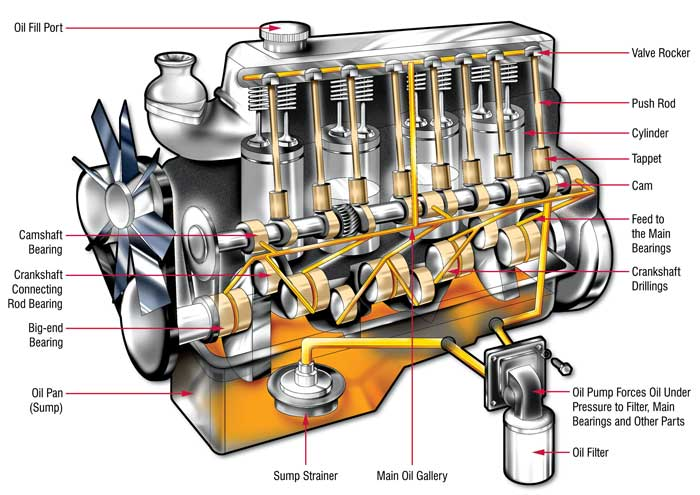
\includegraphics[width=\textwidth, height=8cm]{Motors/motorgasolina.jpg}
     	\caption{Esquema d'un motor de gasolina} 
\end{figure}

Els motors gasolina funcionen en cicles de quatre temps que es podrien classificar, a grans trets, de la següent forma:

\begin{itemize}
  \item Fase d’admissió: La vàlvula d’admissió s’obre, el que permet que la barreja d’aire i combustible flueixi cap a l’interior dels cilindres.
  \item Fase de compressió: Durant aquesta fase, la vàlvula es tanca i el pistó puja per a comprimir la barreja.
  \item Fase d’explosió: Les bugies originen l’espurna necessària per produir l’explosió i el descens dels pistons.
  \item Fase d’escapament: la vàlvula d’escapament s’obre i els pistons \newline s’eleven per expulsar els gasos cremats cap a l’exterior.
\end{itemize}

\subsection{Motors dièsel}
Per norma general, els motors dièsel són principalment emprats en medis de transport que requereixen una dosi extra de potència i que estan pensats per una major càrrega diària de treball, com vehicles industrials, de càrrega, maquinària, medis aeronàutics, etc.
No obstant, des de que aquest tipus de motors naixés de la mà de Rudolf Dièsel en 1893, la tecnologia s’ha estès també cap a medis de transport particulars, arribant actualment a superar en número als vehicles que funcionen amb gasolina.

\begin{figure}[H]
		\centering
    	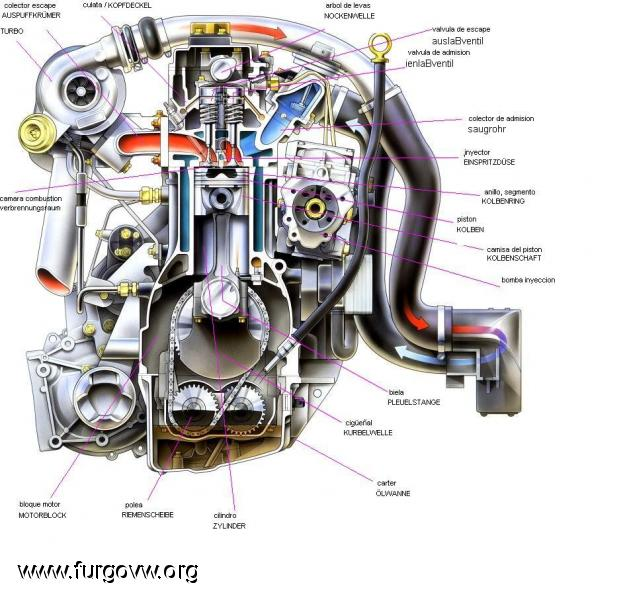
\includegraphics[width=8cm, height=8cm]{Motors/motordiesel.jpg}
     	\caption{Esquema d'un motor diésel} 
\end{figure}

Els motors dièsel funcionen de manera similar als de gasolina i el \newline seu  procés pot dividir-se és d’igual forma en quatre temps, que són els següents:

\begin{itemize}
 		\item Fase d’admissió: Es produeix l'ompliment d’aire i la vàlvula \newline d’admissió roman oberta mentre el pistó descendeix fins el punt\newline mort inferior.
  		\item Fase de compressió: La vàlvula d’admissió es tanca quan el pistó arriba al punt mort inferior i comença el recorregut fins al superior, comprimint l’aire que es troba dintre del cilindre.
  		\item Fase de combustió: L’injector polvoritza el combustible dins de \newline la  càmera i aquest s’inflama d’immediat a l’entrar en contacte amb \newline l’aire  calent.
  		\item Fase d’escapament: S’expulsen els gasos cremats i es deixa que la inèrcia torni a iniciar el cicle.
\end{itemize}

\subsection{Motors de GLP i GNC}
Els vehicles que funcionen amb combustibles alternatius com el GLP (gas liquat del petroli) o el GNC ( gas natural comprimit) van guanyant terreny en la indústria automobilística, i cada cop són més els fabricants que aposten per comercialitzar versions d’alguns dels seus models, propulsats per aquest tipus de combustibles.

\begin{figure}[H]
		\centering
    	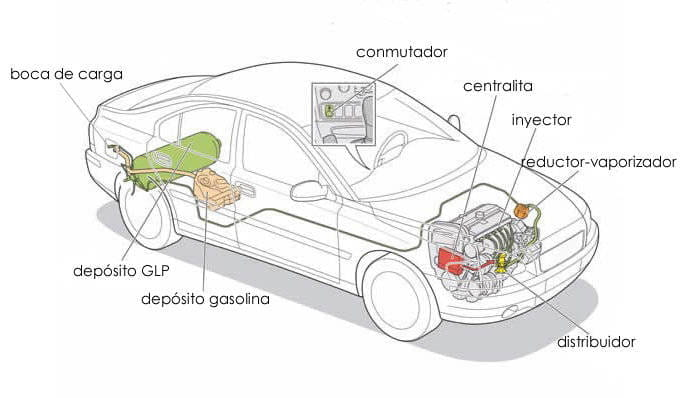
\includegraphics[width=\textwidth, height=8cm]{Motors/motorgnc.jpg}
     	\caption{Esquema de motor gas/gasolina} 
\end{figure}

Qualsevol de les dues opcions, GLP o GNC, afavoreixen l’augment de la vida útil del motor, ja que no generen tant desgast en els cilindres i es depositen menys residus en el sistema. No obstant, s’ha de tindre en compte que en ocasions dificulta la lubricació i pot deteriorar les vàlvules a major velocitat, cosa que podem solucionar gràcies a la mecànica preventiva i realitzant un bon manteniment. 

\subsection{Motors elèctrics}
Encara que no ho sembli, els motors elèctrics són anteriors als dièsel o gasolina de quatre temps. Al 1832 Robert Anderson va desenvolupar el primer automòbil amb motor elèctric pur, capaç de transformar l’energia elèctrica en energia mecànica per medi dels camps magnètics que genera, sense necessitat d’explosions ni combustions pròpies dels motors gasolina i dièsel.

\begin{figure}[H]
		\centering
    	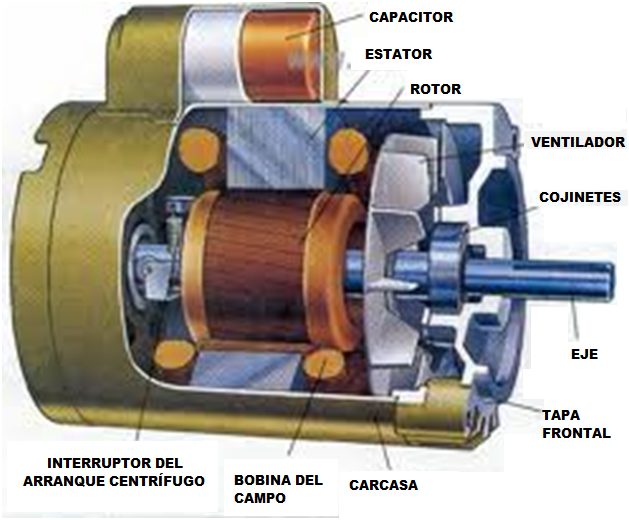
\includegraphics[width=\textwidth, height=8cm]{Motors/motorelectrico.png}
     	\caption{Esquema de motor elèctric} 
\end{figure}

En l’actualitat quan pensem en vehicles elèctrics purs, normalment ens referim a BEV, o vehicles elèctrics de bateria. No obstant, en el mercat podem trobar altres opcions com els FCEV, de pila de combustible, que van combinats amb hidrogen i els HEV i PHEV, coneguts com híbrids i endollables respectivament, que alternen un motor elèctric d’imant permanent amb un de combustió interna (de gasolina principalment). Ja que el nostre controlador serà per a vehicles elèctriques, vol dir que el motor ha de funcionar amb electricitat i per tant, aquest serà el tipus de motor en el qual hi treballarem.

\section{Motors elèctrics}
Els motors elèctrics són màquines elèctriques rotatòries. Transformen una energia elèctrica en energia mecànica de rotació en un eix. Tenen múltiples avantatges, entre els quals cap citar la seva economia, neteja, comoditat i seguretat de funcionament, el motor elèctric ha reemplaçat en gran part a altres fonts d’energia, tant en la indústria com en el transport, les mines, el comerç o la llar.

El seu funcionament es basa en les forces d’atracció i repulsió establertes entre un imant i un fil (bobina) per on circularà un corrent elèctric. Aleshores només serà necessari una bobina (espires amb un principi i fi) un imant i una pila (per a fer passar el corrent elèctric per les espires) per construir un motor elèctric. Per a entendre-ho millor cal saber com funciona l'electromagnetisme.

L'electromagnetisme és la part de la física que estudia les relacions entre el magnetisme i l'electricitat. L'espai on existeixen les forces magnètiques s'anomena camp magnètic. Un camp magnètic el pot generar un imant amb dos pols, pol Nord (N) i pol sud (S). Aquests pols es troben en els extrems del camp que genera l’imant.

\begin{figure}[H]
		\centering
    	
\includegraphics[width=\textwidth, height=8cm]{Motors/campomagnetico.png}
     	\caption{Funcionament del camp magnètic} 
\end{figure}

Tot imant té un camp magnètic i quan el travessa un altre camp magnètic, el d’un altre imant per exemple, els imants es mouen per atracció o repulsió. Si s’apropen dos imants, quan s'ajuntin els camps magnètics generats per cada un d’ells, es mouran. En resum, pols iguals enfrontats es repelen i pols diferents s’atrauen.

No només es pot crear un camp magnètic amb un imant, es pot generar un camp magnètic amb l’electricitat. Les dues forces magnètiques, una del corrent del conductor i l’altre del propi imant, interactuen fent que l’imant giri. En definitiva mitjançant l’electricitat es pot crear el gir d’un eix que en el fons és la funció mecànica que desenvolupen. 

També succeeix al contrari, que es com es construeixen els motors elèctrics de corrent continua.

Si un conductor pel qual circula un corrent elèctric es troba dins d’un camp magnètic, el d’un imant per exemple, el conductor es desplaça perpendicularment al camp magnètic, és a dir, es crea una força en el conductor que fa que aquest es mogui. Realment el corrent que circula pel conductor el que fa és crear al seu voltant un camp magnètic i a l’interactuar el camp de l’imant amb el camp creat en el conductor, es produeix el seu moviment al ser com dos imants. Segons el sentit del corrent del conductor el camp creat tindrà una polaritat o la seva contrària, els camps s’atrauran o repel·liran fent que el conductor es mogui en un sentit o en l’altre.
Si el camp magnètic és horitzontal i el conductor està vertical, el conductor es desplaçarà sortint o entrant de l’imant que provocarà el camp magnètic (depèn del sentit de la corrent pel conductor).

Un cop vists els principis bàsics de funcionament de qualsevol motor \newline elèctric, es mostraran els diferents tipus per tal de veure amb una visió molt major quin seria l'ideal per a enfocar el controlador de vehicles \newline elèctrics per aquest tipus de motor.

\section{Motor de corrent continu}

Van ser els primers en fer-se servir en vehicles elèctrics per les seves bones característiques en tracció i per la simplicitat dels sistemes de control de l'electricitat des de les bateries. Presenten desavantatges en quant al manteniment d'algunes de les peces (escombretes i col·lectors) ja que són motors grans si es busquen potències elevades, doncs la seva estructura (i en concret el fregament entre peces) condiciona el límit de velocitat de rotació màxima. 

Els motors de corrent continu s'utilitzen en casos on és important poder regular contínuament la velocitat del motor, a més a més, s'utilitzen en aquells casos on és imprescindible fer servir corrent directe, com en el cas de motors accionats per piles o bateries. Aquests tipus de motors han de tenir en el rotor i l'estator el mateix nombre de pols i el mateix nombre d'escombretes. Aquests motors poden ser de tres tipus: Sèrie, paral·lel o mixt. 

\begin{itemize}
    \item Motor sèrie: és un tipus de motor elèctric de corrent continu en el qual el bobinat de camp (camp magnètic principal) es connecta en sèrie amb l'armadura.
    \item Motor Paral·lel: és un motor de corrent continu on el bobinat inductor principal està connectat en derivació amb el circuit format pels bobinats induïts e inductor auxiliar.
    \item Motor compost: és un motor de corrent continu on la seva \newline excitació es originada per dues bobines inductores independents; una disposada en sèrie amb el bobinat induït i un altre connectat en derivació amb el circuit format pels bobinats induïts, inductor sèrie i inductor auxiliar. Els motors composats tenen un camp sèrie sobre el límit del bobinat del camp paral·lel. 
\end{itemize}

\subsubsection{Composició}
En primera instància és fonamental senyalar que un motor de corrent continu està composat a grans trets per dues parts. Un estator amb el que se li dóna suport mecànic a l'aparell i és on s'ubiquen els pols de la màquina, que és on quedaran bobinats de fil de coure sobre un nucli de ferro o imants permanents.

Per altra banda està el rotor que quasi sempre és de forma cilíndrica, el qual també està bobinat i amb nucli i s'alimenta amb corrent directe per medi de delgues, les quals estan en contacte de manera alterna amb escombretes fixes.

A mode de resum, en el moment en que un conductor, pel qual està passant corrent elèctrica és submergit en un camp magnètic, aquest conductor sofrirà una força perpendicular al pla que es forma pel camp magnètic i la corrent.

\begin{figure}[H]
		\centering
    	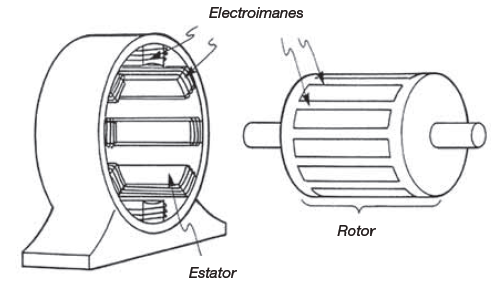
\includegraphics[width=\textwidth, height=8cm]{Motors/rotorestator.png}
     	\caption{Composició d'un motor elèctric de corrent continu}
\end{figure}

\subsubsection{Avantatges}
Encara que el preu d'un motor de corrent continu és considerablement major que el d'un motor d'inducció d'igual potència, existeix una tendència creixent a fer servir motors de corrent continu en aplicacions especials.

La gran varietat de la velocitat, juntament amb la seva facilitat de control i la gran flexibilitat de les característiques par-velocitat del motor de corrent continu, han fet que en els últims anys es faci servir cada cop més amb màquines de velocitat variables en les que es necessiti ampli marge de velocitat i control de les mateixes.

Existeix un creixent número de processos industrials que requereixen una exactitud en el seu control o una gama de velocitats que no es pugui aconseguir amb motors de corrent altern. El motor de corrent continu manté un rendiment alt en un ampli marge de velocitats, el que juntament amb la seva alta capacitat de sobrecàrrega, el fa més apropiat que el de corrent altern per a moltes aplicacions.

\subsubsection{Funcionament}
Quan el corrent passa a través del rotor d'un motor de corrent continu, es genera un par de forces, per la reacció magnètica, i el rotor gira. L'acció del commutador i de les connexions de les bobines del camp dels motors són exactament les mateixes que fan servir els generadors. La revolució del rotor indueix un voltatge en les bobines d'aquesta. Aquest voltatge és oposat en la direcció al voltatge exterior que s'aplica al rotor, i d'allà que es coneixen com voltatge induït o força contraelectromotriu. 

Quan el motor gira més ràpid, el voltatge augmenta fins que és quasi igual a l'aplicat. El corrent aleshores és petit, i la velocitat del motor romandrà constant sempre que el motor no estigui sota càrrega i tingui que realitzar un altre treball mecànic que no sigui el requerit per moure el rotor. Sota càrrega, el rotor gira més lentament, reduint el voltatge induït i permetent que flueixi un corrent major en el rotor. El motor pot així rebre més potència elèctrica de la font, subministrant-la i fent més treball mecànic.

La velocitat a la que funciona un motor depèn de la intensitat del camp magnètic que actua sobre el rotor, així com del corrent d'aquest. Quant més fort és el camp, més baix és el grau de rotació necessari per generar un voltatge induït prou gran com per contrarestar el voltatge aplicat. Per aquesta raó, la velocitat dels motors de corrent continu pot controlar-se mitjançant la variació del corrent del camp.

\begin{figure}[H]
		\centering
    	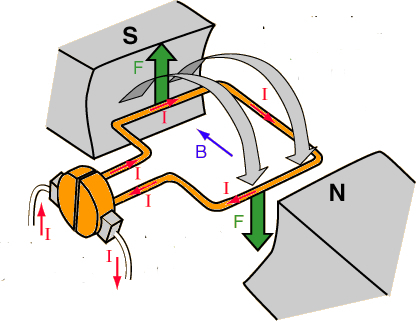
\includegraphics[width=\textwidth, height=8cm]{Motors/funcmotorcontinua.jpg}
     	\caption{Funcionament d'un motor de corrent continu.} 
\end{figure}

En la figura anterior s'explica gràficament el seu funcionament. Es pot apreciar com en el rotor el corrent entra per la part esquerra i per la polarització de l'imant extern fa que el rotor giri en sentit horari. En la següent imatge es pot apreciar les diferents posicions que pot agafar el motor.

\begin{figure}[H]
		\centering
    	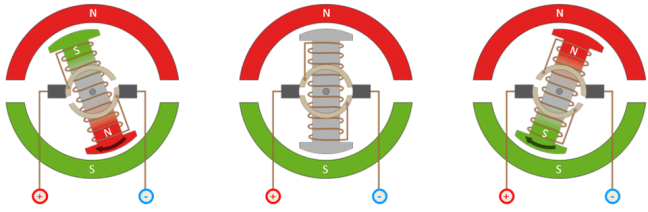
\includegraphics[width=\textwidth, height=6.5cm]{Motors/motorcontinua.png}
     	\caption{Posicions d'un motor de corrent continu.} 
\end{figure}

Els motors de corrent continu són alguns dels motors elèctrics més potents i flexibles. S'utilitzen en ventiladors, arrancadors elèctrics i molts altres aparells. Un motor sèrie DC s'anomena així perquè la bobina de camp i la bobina de rotor estan ambdues connectades en sèrie una amb l'altra. En aquesta configuració el mateixa corrent flueix a través d'ambdues bobines

\subsection{Motors sèrie}
La idea d'aquests tipus de motors és que es connecten a la càrrega en sèrie. El voltatge que s'aplica és constant, mentre que el camp d'excitació augmenta amb la càrrega, donat que el corrent és el mateix corrent d'excitació.

La rotació es pot invertir canviant la direcció del corrent, ja sigui del camp en sèrie o de l'induït.

\begin{figure}[H]
		\centering
    	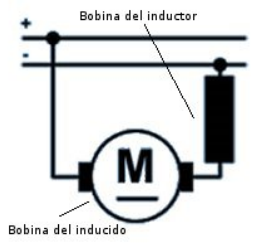
\includegraphics[width=7cm, height=7cm]{Motors/motordcserie.png}
     	\caption{Esquema d'un motor CC en sèrie.} 
\end{figure}

El par produït és directament proporcional al flux i al corrent en l'Induït. El par motor és directament proporcional al quadret de Ia, per tant, la seva corba és parabòlica.

\begin{figure}[H]
		\centering
   	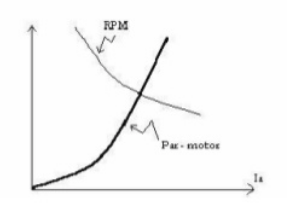
\includegraphics[width=8cm, height=6cm]{Motors/parrpm.png}
     	\caption{Par motor en funció de la intensitat. } 
\end{figure}

\subsubsection{Arrancada i parada del motor}
L'arrancada del motor es produeix intercalant un reòstat d'arrencada en sèrie amb el corrent induït. Aquesta resistència es redueix gradualment quan el motor adquireix velocitat. 

A l'augmentar el corrent per a donar més força a l'arrencada, disminueix la velocitat. Per aquesta raó un motor sèrie ha d'estar sempre engranat o acoplat directament a la càrrega. Si un motor sèrie estigués unit a la càrrega mitjançant una corretja i aquesta es trenqués o es soltés, el motor s'embalaria i molt probablement es danyaria.

Per parar un motor sèrie, és precís introduir progressivament resistències del reòstat d'arrencada i tallar després l'alimentació per evitar un corrent de ruptura agressiu que seria perillós per als enrotllaments

\subsubsection{Velocitat i propietats}
La velocitat es pot variar, canviant el voltatge aplicat, col·locant un reòstat en sèrie amb la bobina de camp. D'aquesta manera es disminueix la velocitat. Es pot augmentar la velocitat, disminuint el flux de corrent per pols. Això es pot realitzar, col·locant un reòstat en paral·lel amb la bobina de camp, de forma que el corrent total només permeti circular una part per la bobina d'excitació.

Les propietats principals d'aquests motors són les següents:
\begin{itemize}
    \item Gran par d'arrencada.
    \item Velocitat variable amb la càrrega.
    \item Tendència a l'accelerament excessiu.
    \item Suporta bé les sobrecàrregues.k
    \item Es dispara fàcilment en el buit o quan la càrrega decreix.
\end{itemize}

Els motors en sèrie tenen aplicacions en aquells casos on es requereix un elevat par d'arrancada a petites velocitats i un par reduït a grans velocitats. El motor ha de tenir càrrega si està en marxa. Alguns exemples serien els tramvies, locomotores, o la majoria de joguines. 

\subsection{Motors paral·lel}

Els trepants són màquines que serveixen per a foradar. Aquestes màquines funcionen amb motors en paral·lel. Però per què? Perquè no poden ser motors en sèrie? Doncs la resposta és evident. En el moment en el que el trepant efectués l'orifici a la peça, la màquina quedaria al buit, és a dir, que no hi hauria cap resistència a la força realitzada al motor. La velocitat a la broca augmentaria tant que arribaria a ser perillós per a l'usuari.

\begin{figure}[H]
		\centering
    	
\includegraphics[width=8cm, height=7cm]{Motors/Motor_paralelo.jpg}
     	\caption{Esquema d'un motor CC amb càrrega en paral·lel} 
\end{figure}

Els motors en paral·lel són uns motors on les bobines estan connectades en paral·lel amb les bobines induïdes. D'aquesta forma, de tot el corrent absorbit pel motor, una part circula per les bobines induïdes i l'altra per les inductores. El circuit d'excitació està a la mateixa tensió que l'inductor (ja que un circuit en paral·lel es manté el voltatge però es redueix la intensitat).

El sentit de rotació d'un motor paral·lel es pot invertir, canviant la direcció del corrent, ja sigui en el circuit de camp o en el circuit de l'induït.

Aquest motor es diferencia amb el motor en sèrie per 3 raons principals:
\begin{itemize}
    \item En l'arrancada, el par motor és menor que en el motor sèrie.
    \item Si la intensitat de corrent absorbida disminueix i el motor està en buit, la velocitat de gir nominal quasi no varia. És més estable que el sèrie.
    \item Quan el par motor augmenta, la velocitat de gir quasi no disminueix.
\end{itemize}

Encara que el motor paral·lel és de velocitat constant, la seva característica més important, és la de ser un motor de velocitat regulable. La velocitat pot augmentar disminuint el flux per pols. Per això, és necessari col·locar un reòstat en el circuit de camp. Per parar el motor s'introdueixen totes les resistències del reòstat d'arrancada abans de tallar el corrent.

Les propietats principals d'un motor paral·lel són les següents:
\begin{itemize}
    \item Par d'arrancada feble.
    \item No suporten grans sobrecàrregues.
    \item Velocitat constant en qualsevol càrrega.
    \item No es disparen en el buit.
\end{itemize}

La velocitat constant d'aquests motors els fa adequats per l'accionament de màquines, eines i aparells d'elevació. S'inclouen tots els casos on no es requereixi un par elevat a petites velocitat i no produeixin càrregues grans, si la càrrega desapareix (en el buit) el motor quasi no varia de velocitat.

\subsection{Motor mixt}
El motor mixt és una combinació del motor sèrie i el motor paral·lel,  donat que una de les bobines inductores està en sèrie amb l'induït, mentre que l'altra està en paral·lel amb ell. Una part de la intensitat de corrent absorbit circula per les bobines induïdes i, per tant, per una de les inductores; mentre que la resta del corrent recorre l'altra bobina inductora. 

\begin{figure}[H]
		\centering
    	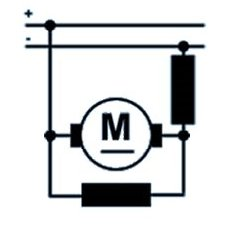
\includegraphics[width=8cm, height=8cm]{Motors/Motor_compuesto.jpg}
     	\caption{Esquema d'un motor CC amb càrrega en paral·lel.} 
\end{figure}

Comparant els avantatges dels motors sèrie i paral·lel es troba que el motor paral·lel té una major velocitat constant, però un motor sèrie de la mateixa capacitat pot exercir un par molt major, quan és necessari, sense augmentar terriblement el corrent. Aquestes dues característiques poden obtindre's en un mateix motor col·locant dos bobinats de camp: Un en sèrie i l'altre en paral·lel en els pols del motor. És per això que es denominen motors mixts. 

La velocitat d'un motor compost es pot disminuir per sota la normal \newline mitjançant un reòstat col·locat en el circuit de l'induït i augmentar per sobre de la normal mitjançant un reòstat en el circuit de camp. A diferència dels motors en sèrie, el motor compost té una velocitat definida sense càrrega i no arribarà a velocitats destructives si aquesta es suprimeix. La regulació de la velocitat és inferior a la d'un motor paral·lel i major a la d'un sèrie. La rotació s'inverteix canviant la direcció del corrent del circuit de camp o del circuit induït. Donat que si s'inverteix el camp paral·lel s'ha d'invertir el sèrie, el procediment més simple és invertir el corrent en l'induït.

\section{Motor de corrent altern}

Es denomina motor de corrent altern aquells motors elèctrics que funcionen amb corrent altern. Un motor és una màquina motriu, això és, un aparell que converteix una forma determinada d'energia en energia mecànica de rotació o par. Un motor elèctric converteix l'energia elèctrica en força de gir per mitjà de l'acció mútua dels camps magnètics.

Els motors de corrent altern es classifiquen per la seva velocitat de gir, pel tipus de rotor i pel nombre de fases d'alimentació:
Existeixen 4 tipus:

\begin{itemize}
    \item Motor universal: Pot treballar tant en CA com en CC: L'ús d'aquests motors en corrent altern està molt estès pel major par d'arrancada respecte al dels motors d'inducció i per la seva elevada velocitat de rotació, el que permet reduir la seva mida i el seu preu. Així, s'empren en màquines com eines portàtils de tot tipus, \newline electrodomèstics petits, etc.
    \item Motor asíncron: Són un tipus de motor de corrent altern en el que el corrent elèctric, en el rotor, necessari per produir torsió és induït per inducció electromagnètica del camp magnètic de la bobina de l'estator. Per tant un motor d'inducció no requereix una commutació mecànica apart de la seva mateixa excitació o per tota o part de l'energia transferia de l'estator al rotor, com en els universals, DC i motors grans síncrons.
    \item Motor síncron: Els motors síncrons són un tipus de motor de corrent alterna en el que la rotació de l'eix està sincronitzada amb la freqüència del corrent d'alimentació; el període de rotació és exactament igual a un nombre enter de cicles de CA.
    \item Motor de gàbia d'esquirol: La major part dels motors que funcionen amb CA d'una sola fase tenen el rotor de tipus gàbia d'esquirol. Els rotors de gàbia d'esquirol reals són molt més compactes i tenen un nucli de ferro laminat.
\end{itemize}

\subsubsection{Composició}

De la mateixa forma que amb els motors de corrent continu, aquests motors estan composats a grans trets per dos components principals: el rotor i l'estator. 

El circuit magnètic dels motors elèctrics de corrent altern està format per xapes magnètiques i aïllades entre elles per eliminar el magnetisme permanent.

El circuit magnètic està forma per xapes apilades en forma de cilindre en el rotor i en forma d'anell a l'estator. El cilindre s'introdueix a l'interior de l'anell. L'anell es dota de ranures en la seva part interior per col·locar el bobinat inductor i s'embolica exteriorment per una peça metàl·lica amb suport, la carcassa.

\subsection{Motor universal}
S'anomena així per ser l'únic motor que pot connectar-se tant a corrent altern com a corrent continu. Quan el motor es connecta al corrent continu amb una càrrega constant, la velocitat i la potència augmenten proporcionalment amb el voltatge aplicat.

Quan aquest motor es connecta al corrent altern amb càrrega constant, la velocitat i la potència augmenten proporcionalment amb el voltatge aplicat.

En el motor universal la velocitat donada per un voltatge en corrent altern és inferior que la que s'obtindrà si s'aplica el mateix voltatge però en corrent continu. Els motors universals es construeixen per potències menors a mig cavall de potència i velocitats de fins a 3000 rpm i presenten un bon rendiment.

El principi de funcionament d'aquest motor elèctric està determinat per l'efecte motor que produeix un conductor recorregut per un corrent \newline elèctric i que està sotmès a un camp magnètic. Per acció magnetomotriu existirà un desplaçament i per tant es produirà una rotació.

El motor universal està composat pels següents components:
\begin{itemize}
    \item Bobines conductores.
    \item Bobines induïdes.
    \item Escombretes.
    \item Ressorts.
    \item Tapes o escuts.
\end{itemize}

\begin{figure}[H]
		\centering
    	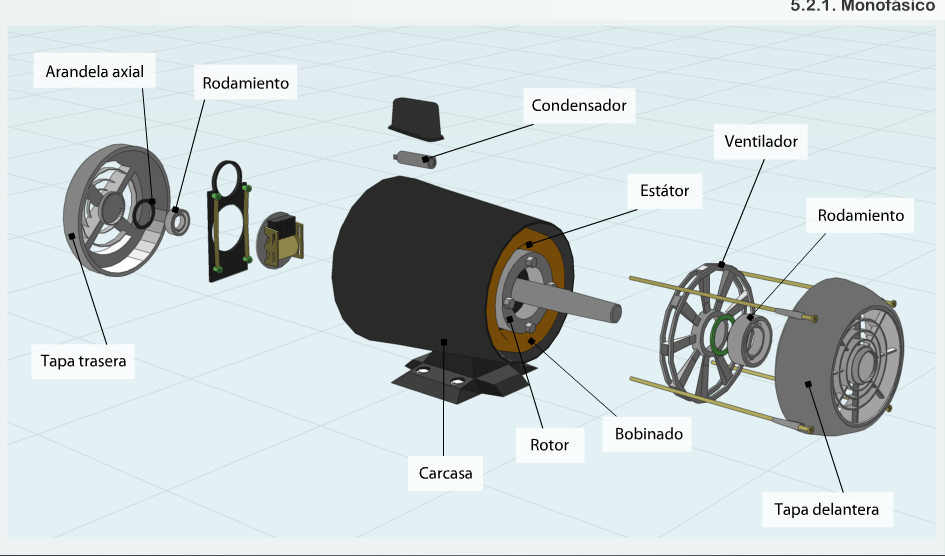
\includegraphics[width=\textwidth,height=8cm]{Motors/composicionmotoruniversal.png}
     	\caption{Constitució d'un motor universal.} 
\end{figure}

Les característiques principals d'aquests tipus de motos són les següents:
\begin{itemize}
    \item Funciona amb corrent altern i corrent directe.
    \item Posseeix un par d'arrancada molt elevat.
    \item Per invertir el sentit de rotació, s'inverteix el sentit del corrent en qualsevol dels bobinats.
\end{itemize}

El motor elèctric basa el seu funcionament en la llei de Laplace. El bobinat inductor i el bobinat induït estan connectats en sèrie. Al ser recorreguts per un corrent, el bobinat inductor forma el camp magnètic i l'induït per la llei de Laplace, al ser recorregut pel corrent i sotmès a la influència del camp magnètic inductor, es desplaça, donant origen al gir del rotor.

Si augmenta el camp augmenta la força i la velocitat. El camp magnètic que produeix la bobina induïda provoca una deformació del flux inductor anomenat reacció de l'inductor. En corrent altern o en corrent continu el sentit es manté per l'acció de cada alternança en particular. En corrent altern es produeix una força contraelectromotriu per efecte transformador i per efecte generador. En corrent continu només per efecte generador.

Com en la majoria de motors la regulació es pot establir mitjançant reòstats o per commutació de resistències

\subsection{Motor síncron}
Una màquina sincrònica és una màquina de corrent altern on la seva velocitat és proporcional a la freqüència del corrent. El camp magnètic que creen els corrents de l'armadura gira a la mateixa velocitat que el que crea el corrent de camp en el rotor, i es produeix un par estacionari.

Aquests motors són màquines rotatòries elèctriques que poden treballar tant com motor com generador. Com a motor es converteix l'energia \newline elèctrica en energia mecànica i viceversa com a generador. Aquestes \newline màquines no tenen par d'arrancada i s'ha d'emprar diferents mètodes d'arrancada i acceleració fins la velocitat nominal de sincronisme.

Les màquines sincròniques s'utilitzen en major mesura com generadors de corrent continu que com motors de corrent altern. La màquina tipus síncrona més estesa és l'alternador, que és l'aparell que s'encarrega \newline d'aprofitar l'energia mecànica que genera un cotxe i convertir-la en energia elèctrica per a carregar la bateria del propi cotxe.

\begin{figure}[H]
		\centering
    	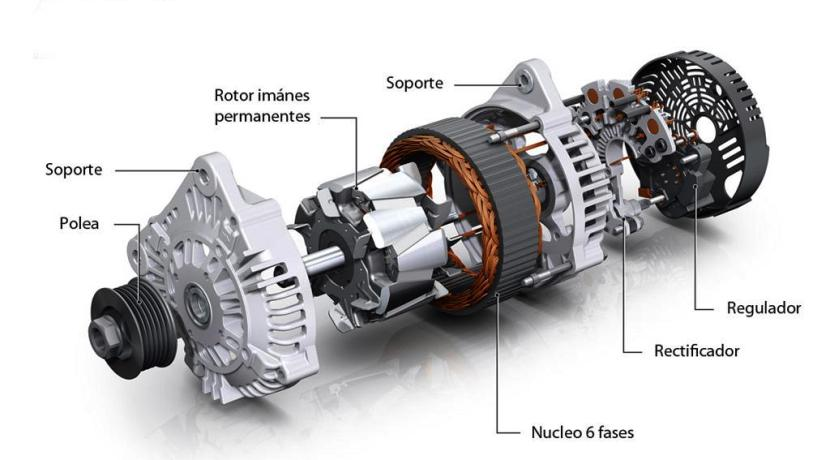
\includegraphics[width=\textwidth,height=8cm]{Motors/alternador.jpg}
     	\caption{Esquema d'un alternador.} 
\end{figure}


A nivells de construcció, són molt similars a la majoria de motors, formant-se per un rotor i un estator. L'estator és completament igual que el d'un motor asíncron però és al rotor on hi apareixen certes diferències. Aquest rotor conté un debanament de corrent continu, denominat debanament de camp i un debanat en curtcircuit, que impedeix el funcionament de la màquina a una velocitat diferent a la de sincronisme, denominat debanament amortidor. A més a més, conté un circuit magnètic format per apilament de xapes magnètiques de menor gruix que les de l'estator.

Les principals avantatges que presenten són les següents:
\begin{itemize}
    \item És l'única màquina que ofereix garantia en la estabilitat de la velocitat.
    \item Tenen un molt bon rendiment.
    \item Poden fer-se servir com a dispositius de correcció del factor de \newline potència. El factor de potència es controla variant l'excitació del rotor.
    \item Poden ser connectats directament a una xarxa d'alta tensió sense necessitat de transformador intermedi.
    \item Possibilitat de funcionar com generador de potència reactiva.
    \item Subministrament de potència a càrregues que treballen a velocitat constant.
    \item El voltatge en els terminals i la freqüència del sistema seran constants, independentment de la quantitat de potència presa pel motor.
\end{itemize}

Per entendre millor el funcionament dels motors síncrons cal tenir clar que la velocitat és proporcional a la freqüència del corrent de l'armadura i que el camp magnètic creat pels corrents de l'armadura giren a la mateixa velocitat que el que crea el corrent de camp en el rotor. 

Els pols del rotor estan sotmesos a atraccions i repulsions, en breus \newline períodes de temps, per part dels pols de l'estator, però el rotor no aconsegueix girar fins arribar a la velocitat de sincronisme. 

\begin{figure}[H]
		\centering
    	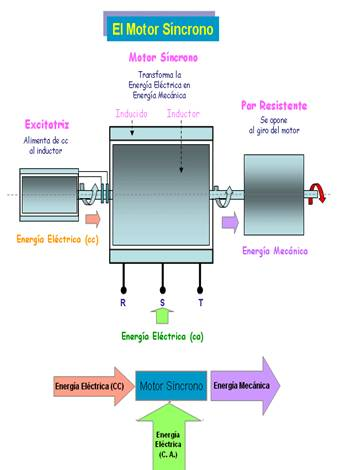
\includegraphics[width=8cm,height=8cm]{Motors/funcionamientomotorsincrono.jpg}
     	\caption{Funcionament d'un motor síncron.}
\end{figure}

\subsection{Motor asíncron}
Els motors asíncrons o d'inducció són motors de corrent altern en els que el corrent elèctric que es necessita per produir la torsió del rotor és induïda per inducció electromagnètica del camp magnètic de la bobina de l'estator. D'aquesta forma, els motors asíncrons no necessiten una commutació \newline mecànica com succeeix en els motors síncrons i els motors de corrent continu.

Els motors asíncrons estan constituïts principalment per dues parts: 
\begin{itemize}
    \item Circuit magnètic: La part fixa del circuit magnètic (estator) és un anell cilíndric de xapa magnètica ajustada a la carcassa que l'envolta. La carcassa té una funció purament protectora. 
    \item Circuits elèctrics: Els dos circuits elèctrics van situats un en les ranures de l'estator i l'altre en les del rotor, que està curtcircuitat. 
\end{itemize}

\subsection{Motor pas a pas}
Els motors pas a pas són un tipus especial de motors que permeten l'avenç del seu eix en angles molt precisos i per passos en les dues possibles direccions de moviment. Aplicant a ells una determinada seqüència de senyals digitals, avancen per passos cap a un costat o l'altre i es detenen exactament a una determinada posició.

Cada pas té un angle molt precís determinat per la construcció del motor, el que permet realitzar moviments exactes sense necessitat d'un sistema de control de llaç tancat.

A un motor pas a pas se li pot ordenar per medi del control, que avanci cinc o deu passos cap a la dreta, després un determinat nombre de passos cap enrere o simplement que no giri, el qual permet el control de la posició, velocitat i sentit. Aquest sistema ha simplificat enormement la implementació \newline d'automatismes i les aplicacions de la robòtica.

Els motors pas a pas presenten grans avantatges respecte a la utilització de servomotors degut a que es poden manejar digitalment sense realimentació, la seva velocitat es pot controlar fàcilment, tenen una llarga vida, són de baix cost, la interfície és senzilla i el seu manteniment és mínim degut a que no tenen escombretes.

El funcionament dels motors pas a pas es basa en el simple principi \newline d'atracció i repulsió que succeeix entre els pols magnètics. 

Per aconseguir un moviment molt més suau, els motors pas a pas es fabriquen augmentant el nombre de pols de l'estator amb una sèrie de ranures tant en el rotor com en l'estator. Així s'aconsegueixen moviments que van fins a 1.8º/pas. Els graus d'avenç per pas són una de les característiques més important en aquest tipus de motors i generalment està indicada en el seu cos.

Els motors PAP tant unipolars com bipolars poden treballar en dos modes d'operació: de pas complert i de mig pas.

En el primer cas, amb cada seqüència el rotor gira un determinat angle donat per la fabricació del motor. En el mode de mig pas, cada seqüència produeix un gir en graus corresponent a la meitat del seu pas normal. 



\subsection{Motor d'imants permanents}
En general el camp magnètic d'un motor DC es pot produir per bobines o imants permanents. Els motors DC d'imant permanents es poden classificar dacord amb l'esquema de commutació i al disseny de l'armadura. Els motors DC convencionals tenen escombretes mecàniques i commutadors. No obstant, en una clase importants de DC la commutació es fa de forma electrònica; aquest tipus de motor s'anomena motor DC sense escombretes.

El flux magnètic produït per l'imant passa a través de l'estructura del rotor laminat amb ranures. Els conductors de l'armadura estan localitzats en les ranures del rotor. Aquest tipus de motor està caracteritzat per una inèrcia del motor relativament alta (ja que la part giratòria està formada per les bobines de l'armadura), una inducció alta, baix cost i alta confiabilitat.

Els conductors de l'armadura estan enganxats a la superfície de \newline l'estructura cilíndrica del rotor, la qual està feta de discs laminats agafats a l'eix del motor. Ja que en aquest disseny no s'empren ranures sobre el rotor, no presenta l'efecte de "roda dentada". Donat que els conductors estan projectats en el entreferro d'aire que està entre el rotor i el camp d'imants permanents, aquest camp té menor inductància que el d'estructura de nucli de ferro.

\section{Motors Brushless}
Els motors brushless són uns motors trifàsics que funcionen mitjançant la commutació de les bobines per el controlador, això ens dóna pràcticament il·limitades revolucions ja que no es limiten unes escombretes a l'hora de commutar las bobines del rotor i estator. Aquests motors necessiten poc manteniment ja que no hi ha peces sotmeses a desgast pel fregament. Tenen una corba de velocitat par plana i poden realitzar el seu par en pràcticament totes les revolucions que en permet el motor. El fet de no tenir baixades de voltatge per la commutació les bobines i el bobinat en l'estator, permet obtenir motors molt més petits amb la mateixa potència. El control de motor es complica ja que la commutació de les bobines es fa mitjançant el controlador i no mecànicament. El fet de ser un motor complex suposa un cost de la construcció del motor i fa que sigui un motor car ja que conté un rotor d'imants permanents.

\subsection{Paràmetres dels motors brushless}

Paràmetres a tenir en compte del motor brushless per fer una selecció correcta del motor que necessitem:\smallskip

\subsubsection{KV}
És un dels paràmetres més importants per la selecció del motor, tot i que en el marcat trobem motors amb la mateixa potència, voltatge i intensitat, però amb diferents KV. A termes generals són les voltes per voltatge que té el motor, es a dir, pel mateix motor les baixes versions de KV tenen més bobinats amb filferro més prim, mentre que les altes versions de KV tenen menys bobines amb filferro més gruixut. Sempre que tinguin la mateixa massa de coure, són exactament iguals pel que fa a la potència màxima de sortida, parell, eficiència i revolucions màximes.\smallskip
    
Poden haver diferents versions KV del mateix motor ja que són totalment equivalents. El KV només afecta al sistema de control i de bateria i per tant, mentre comparem els motors, permet parlar de parell en comptes de corrent perquè el parell és proporcional al corrent / KV i, el valor de KV es pot canviar lliurement amb la quantitat de voltes i el gruix del coure.\bigskip
     
\subsubsection{Sensored i Sensorless}

Depenen de com dissenyem el controlador podrem controlar els motors Sensorless o Sensored o els dos, per això cal veure com funciona l'excitació de les bobines del motor brushless.\smallskip
    
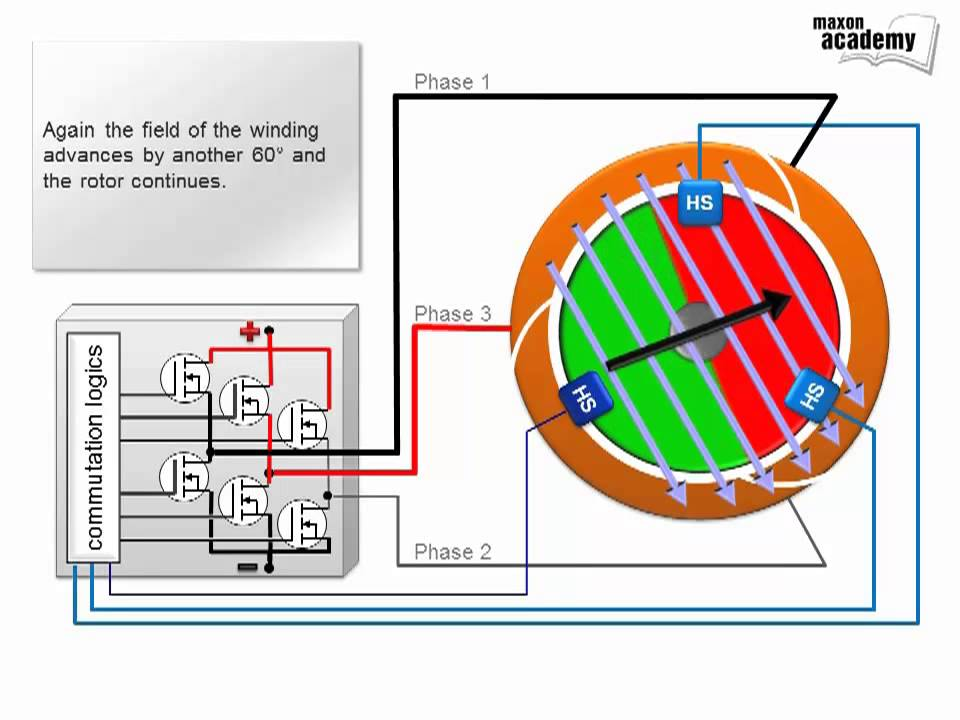
\includegraphics[width=\textwidth]{bobinas}
    
En la imatge es pot veure l¡esquema d'un motor Sensored en el qual porta 3 sensors d'efecte hall per tal de veure el camp magnètic del rotor. A partir d'aquesta informació es pot saber quina orientació té el motor respecte el camp generat per les bobines i alternar a la següent bobina per continuar el gir en la posició òptima. En el cas del Sensorless que no disposa dels sensors d'efecte hall es farà una estimació a partir de la intensitat consumida i els polsos enviats anteriorment. A altes velocitats de rotació l'efecte es poc pronunciat però a baixes velocitats és molt probable que no s'estigui optimitzant el consum del motor ja que s'alterna abans o després del punt ideal de les bobines. Això provocarà un consum extra de potència en les bateries, arribant a sobreescalfar els controlador del motor. 

\subsection{Com funciona el motor Brushless}
Com el seu nom indica són motors sense escombretes, en aquest tipus de motor la corrent passa directament per les bobines creant un camp magnètic que interacciona amb el camp creat pels imants permanents del rotor, per tant el control de les bobines generen el camp i com el movem per produir el gir desitjat el deleguem al variador, per això els sistemes de control són més complicats. Aquest és capaç per uns sensors o pel comportament del corrent determinar la posició magnètica del rotor i modificar el camp magnètic generat per obtenir la força de gir desitjada.
    
Per aconseguir que el motor comenci a girar ha d'induir un camp \newline magnètic a les bobines perpendicular al camp dels imants del rotor, en aquestes condicions el par serà el màxim, és el que en interessa en tot moment, si en algun moment volguéssim menor par disminuiríem la potència del camp però intentaríem fer servir el màxim perpendicularment possible per fer-ho al màxim de eficient.\smallskip
    
En tot moment la posició del rotor és variable, per tant ens hem de dotar de sistemes que ens facilitin saber la posició del rotor per saber com s'han d'excitar les bobines. Aquí disposem de dos estratègies; sensorless (sense sensors) o sensored (amb sensors). Els motors sensored disposen \newline d'elements que ens informen de la posició del camp magnètic o orientació del rotor en tot moment. En el cas dels motors sensorless no es disposa de cap sistema que mostri la posició del camp, normalment es mesuraran els polsos d'intensitat i veient com es comporten es suposarà l'orientació del rotor. Solen ser sistemes més econòmics ja que no tenen un cost de sensors.

\section{Control de motors elèctrics}

Depenen del tipus de motor que tinguem tindrem mesures de control diferents per adaptar-se al motor en qüestió. Dintre de cada tipus de control de motor té diverses formes de ser controlat per tal de simplificar la instal·lació limitant el control d'aquest o controlant tots els aspectes del propi motor. 

Per a parlar dels algorismes de control primerament cal fer una gran diferenciació dels dos grups que hi apareixen; els de llaç obert i els de llaç tancat. La diferència és que els primers no tenen realimentació a un control i els segons sí. Cal veure que depenen del tipus de motor el control amb llaç obert o tancat proporcionarà diferents efectes. 

En el llaç obert nomes apliquem una consigna a la nostra sortida i no tenim en compte que a la realitat aquesta consigna no es realitzi i per tant, s'estigui realitzant un moviment incorrecte. Només es pot confiar en la consigna donada.

En el control de llaç tancat es munta algun tipus de sensor que torna a enviar a un control la informació que realment està reben el motor. Pot ser la velocitat, la intensitat, el parell o la posició. En aquest control si es dóna una ordre X i ens retorna un valor de X-2, el següent enviament enviarem X+2 per compensar aquesta variació. D'aquesta forma és molt més precís aconseguir aquesta consigna.

Els algorismes de control que es tractaran seran els algorismes de llaç tancat, concretament els que es basen en motors amb PID.

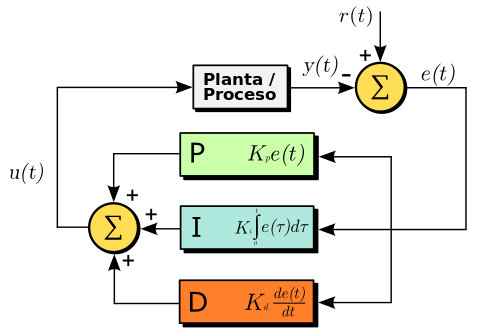
\includegraphics[width=\textwidth]{Motors/PID}

El PID està format per 3 etapes principals les quals són les que es troben si es desglossa l'acrònim PID; Proporcional, Integral i Derivatiu.

Es basa en agafar la resposta del sensor i restar-la a la consigna, aplicant les 3 etapes per donar el senyal més precís al motor, per aconseguir la consigna. El paper que juguen en el control es mostra en els següents punts: 

\begin{itemize}
    \item Proporcional: El control proporcional es basa en multiplicar l'error per una constant per determinar la sortida, és a dir, si estem molt lluny de les consignes donarà una sortida molt gran per aproximar-nos al senyal de referència, però un cop estiguen en aquesta pararà el control donant sortida 0. Això es pot provar una oscil·lació si el valor és molt gran o una no correcció ja que ha de mantenir un error constant per tal d'adaptar-se a la mesura.
    
    \item Integral: Con el seu nom indica es basa en realitzar la integral del senyal d'error. En el cas anterior l'error es manté constant en un valor concret. El control integratiu anirà pujant de valor fins a corregir el problema, és un control que si no es limita provoca moltes oscil·lacions en el control. 
    
    \item Derivatiu: És el que realitza la derivada de l'error per tal de controla el motor. És un control útil en el cas de pertorbacions externes, és a dir, en el cas que arribi una pertorbació externa que es desvia de l'objectiu la derivada corregirà molt i provocarà ràpides i curtes reaccions en el control per tal d'intentar tornar el com mantenint la posició.
\end{itemize}    
    
\subsubsection{Generació d'un senyal PWM}
Una ona PWM es pot generar de forma digital o amb circuiteria electrònica. El més utilitzat és la forma digital amb microcontroladors per tal de facilitar el control. El seu funcionament es basa en un comptador del microcontrolador que es programa de forma que vagi incrementant un valor fins arribar al màxim i que torni a començar pel 0. Això ens donarà el període del senyal PWM. Una vegada tenim el període ens falta el temps d'ON, això ho regularem amb una variable que es compararà amb un valor de temps. Sempre que estigui per sobre engegarem la sortida, això ens provoca que puguem canviar la consigna en tot moment arribant a generar polsos estranys, per això el que farem serà que la consigna només es pugui canviar en el punt més alt o ms baix del comptador.

\subsection{Motor de CC amb escombretes }

Aquests tipus de motors són motors que la seva velocitat depèn directament del voltatge es es posi en els seus terminals i el seu parell depèn del propi motor i de la intensitat que hi circula.

Per un control senzill d'aquest tipus de motors és realitza mitjançant un interruptor, o un relé o un transistor que permetrà controlar el motor en un sentit determinat a la velocitat determinada. No es podrà controlar el motor en un sentit determinat a la velocitat a la que gira. A més a més hi haurà una única marxa i serà constant. Cal destacar que el no controlar la intensitat del motor suposarà un esforç massa gran. Podria provocar que la intensitat es disparés, arribant a cremar el motor. Per evitar això aquest tipus de motors es protegeixen amb fusibles.


Control complet d'un motor de cc, em de fer servir la t'encinca de pont en H per tal de controlar la velocitat i el sentit de gir\smallskip

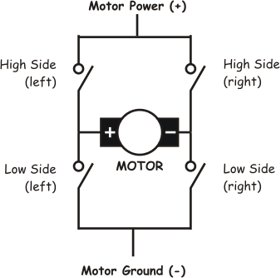
\includegraphics[width=\textwidth]{Motors/basic-bridge}

Controlar amb interruptors l'estat de HIGH i LOW podent fer veure que el motor està connectat en els dos sentits per tal de poder controlar la seva direcció. Aquest esquema també es pot realitzar mitjançant relés si no es volgués controlar la velocitat i la intensitat.

per controlar la velocitat a la qual fem girar el motor nesesitem fer el pont en transitors i controlar el dispar mitgagent honas PWM per tal de controlar el voltage que veu el motor: \smallskip

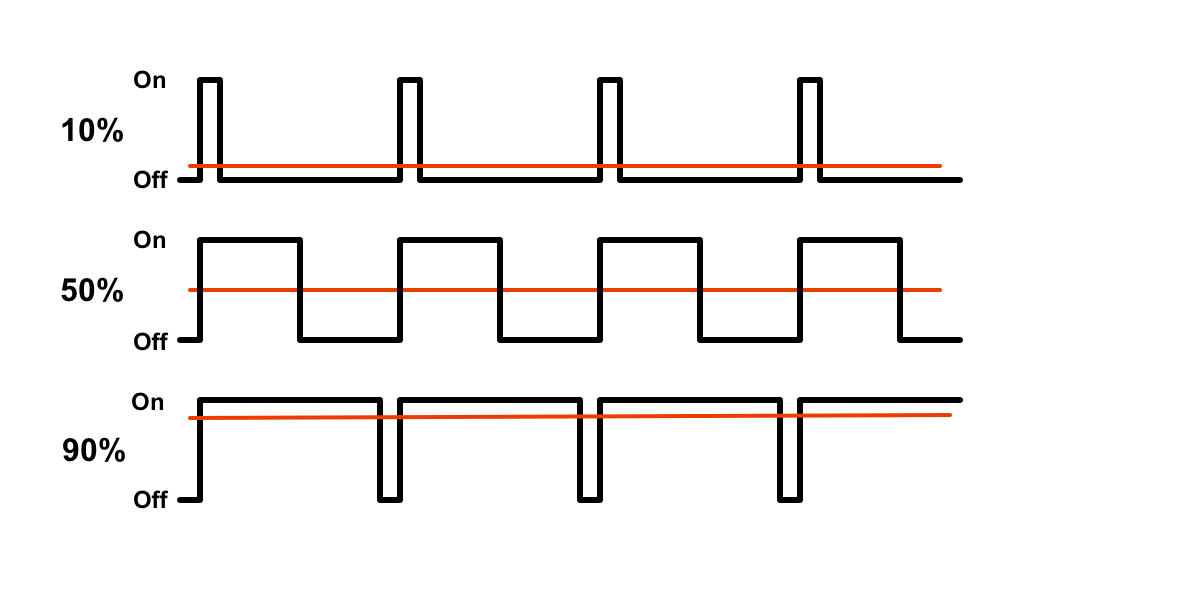
\includegraphics[width=\textwidth]{Motors/PWM}

Mitjançant una ona quadrada a una freqüència determinada, es podrà controlar el percentatge de l'ona que és el temps que l'ona es troba en estat HIGH i en LOW dins d'un mateix cicle. Es podrà donar doncs polsos amb el cicle complert a HIGH o complert a LOW lo suficientment ràpid com per que el motor treballi a voltatge constant, per variacions en la càrrega es pot variar la velocitat del motor, per tant es munten controls PID per tal d'anar adaptant la sortida del pont mantenint la velocitat controlada.

Amb el control de voltatge tindrem el control de la velocitat i el sentit. Pràcticament tindrem tot el control total del motor, encara que segueix havent el perill de cremar-lo. Per això es munta un segon sistema de control que controla la intensitat subministrada al motor per tal de tenir la força que crea la intensitat controlada. És munta doncs un PID per tal de poder saber la intensitat real que està arribant al motor per tal de modificar el cicle de l'ona per reduir-la o augmentar-la per tal de controlar la força realitzada pel motor.

Existeixen problemes amb el pont de potència, el pont en H. En el cas que volguéssim controlar el pont en forma de transistors i amb ones PWM, no ens podríem basar només en controlar els interruptors en creuat, ja que un motor està format per bobines i al tallar de cop la circulació de corrent el voltatge es podria disparar, arribant a cremar els transistors. Per tant cal controlar el pont mitjançant 4 sortides i no 2 com es donaria a entendre, a part s'hauran de connectar díodes de contrapolaritat entre el positiu i el negatiu del motor per a que deixi de fluir corrent invers. Les etapes d'aquest procés serien les següents:

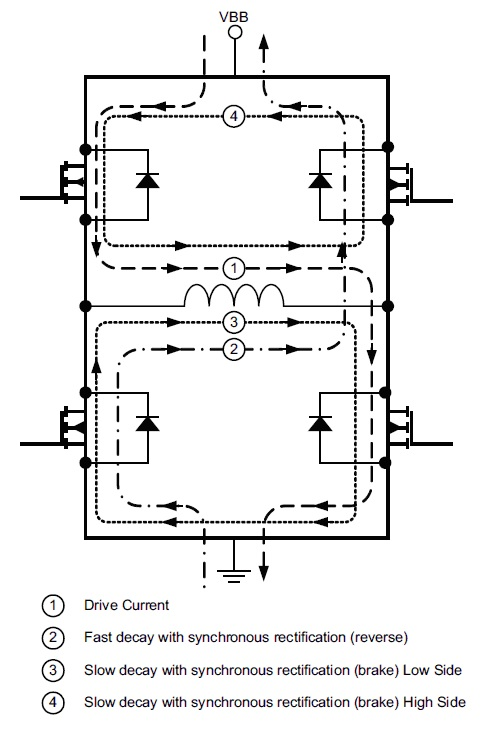
\includegraphics[width=\textwidth]{Motors/Hsteps}
\bigskip

\begin{enumerate}
    \item Control de corrent per polsos per tal de subministrar corrent al circuit. Recordar deixar el pont en H obert per facilitar el pas de corrent i que no \newline apareguin tensions molt altes que pugin cremar el pont. 
    \item Es deixarà que el corrent del motor passi pels díodes per tal de disminuir el corrent del motor i que el voltatge no es dispari i pugi cremar els transistors. Això succeirà si es manté una frenada progressiva del motor i una desacceleració. Es pot accelerar connectant els mosfets contraris per tal d'accelerar la frenada però pot produir una acceleració a l'invers. 
    \item La circulació de corrent per al estat LOW o HIGH es basa en deixar un dels dos mosfets inferiors o superiors activats per tal de provocar el bucle de corrent i desaccelerar ràpidament el corrent de motor.  
\end{enumerate}

\subsection{Motors de corrent altern}

En el control de motors de corrent altern la seva velocitat no ve definida pel voltatge que li apliquem directament sinó que ve definida per la freqüència de commutació de la xarxa. Per això existeixen dos maneres de controlar-ho; entrant a la xarxa per contactor que dóna directament el voltatge o bé en un circuit amb contactors que ens permet canviar el sentit de gir invertint una de la seves fases. En els cassos del trifàsics amb arrancada estrella-triangle que són les dues potències que pot tenir un motor, s'arrencarà per la part menys potent i anirà cap a la més potent amb el motor en marxa.


\subsubsection{Control mitjançant un variador de velocitat}
En el control per variació de velocitat necessitarem una font de corrent continu en el voltatge de pic del motor altern. Una vegada tinguem aquesta, muntarem un inversor trifàsic o monofàsic per tal d'emprar l'ona PWM i generar un pseudo-senyal sinusoïdal en el qual podrem controlar la seva freqüència, el seu voltatge i la intensitat de forma que puguem determinar la potència del motor per no cremar-ho i la freqüència per determinar el sentit i velocitat de gir.

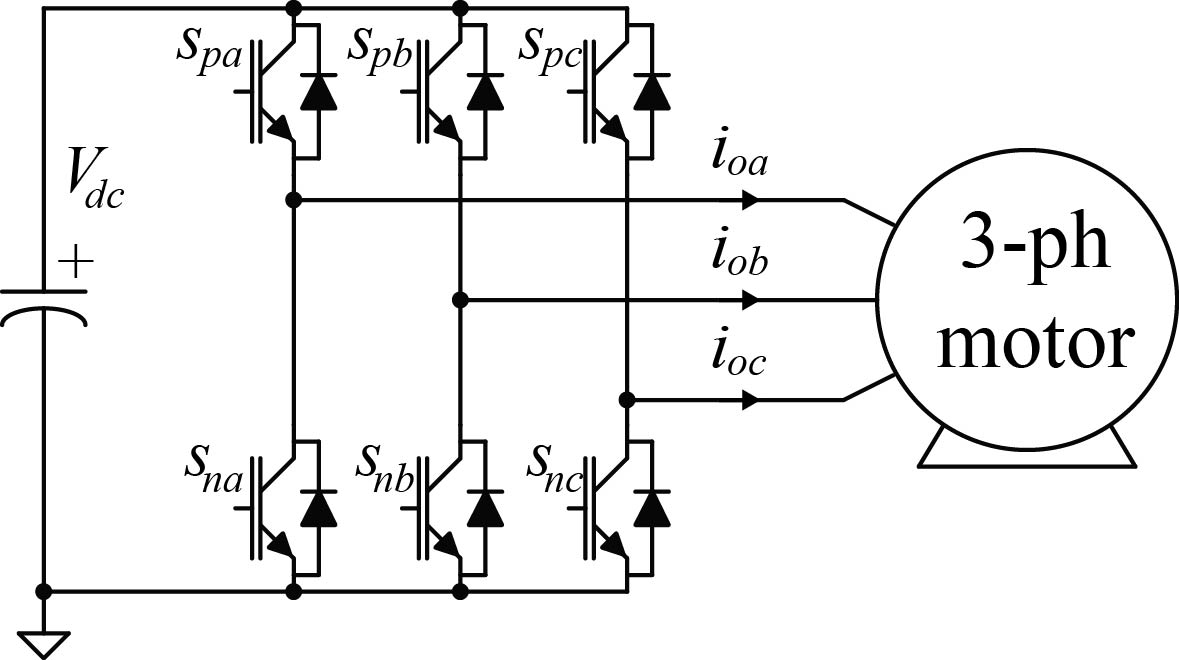
\includegraphics[width=\textwidth]{Motors/inverter}

A part de controla les variables en qüestió existeixen alguns paràmetres més que poden ser interessants com per exemple el fre per injecció de CC que consisteix en fer circular corrent continu en el motor per tal de generar un camp magnètic fix i produir una frenada molt forta del motor.

\subsection{control de motors pas a pas }

En el control de motors pas a pas disposem de bobines repartides pel motor amb connexió exterior, per norma general està composat per 2 bobinats alterns. El control normal és de llaç obert però també disposen de llaç tancat. El que fem per controlar aquest tipus de motor és activar les bobines des d'un microcontrolador fixant la posició del Stepper en una bobina o combinació d'aquestes conegut com a microstepping.

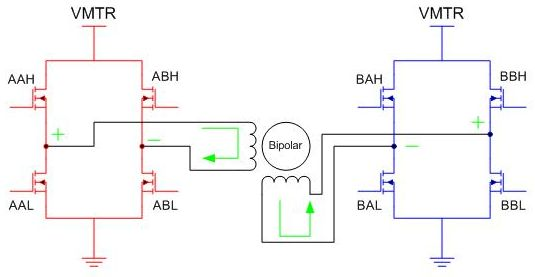
\includegraphics[width=\textwidth]{Motors/stepers.jpg}

Aquí només hem de controlar la intensitat que va a cada bobina per tal de no cremar-les. Una vegada controla la intensitat el que cal fer és invertir el voltatge de les bobines i les bobines activades, per tal d'anar canviant la posició del Stepper a la posició desitjada. Un problema comú és quan el motor està proper al parell que pot generar i es perden passos, és a dir, el motor es salta una bobina per culpa del parell resistiu que té en l'eix. La forma de solucionar-ho és aplicant un motor més potent o fent que el control sigui de llaç tancat. Un exemple d'un d'aquests motors en llaç obert és la impressora 3D.

El control dels ponts en H és molt similar al control que tenim en els motors de CC intentant mantenir una intensitat constant. Normalment s'utilitzen integrats per facilitar les feines com els DRV8825 \footnote{https://www.pololu.com/product/2133} o altres similars, aquests drivers el que fan és simplificar-nos el control en, enable per activar els bobinats de pas i direcció pel control. També podem configurar el microstepping fins a 1/32 o múltiples inferiors

\subsection{Controls de motors brushless}
Un motor brushless es controla d'una forma molt similar a un motor de CC però amb algunes complicacions. En comptes d'1 bobinat que va canviant per l'efecte de les escombretes, ara en tenim 3 i en comptes de escombretes per generar l'imant interior tenim un imant permanent. Això provoca que la velocitat vagi lligada als voltatges de les fases, però no pot ser constant ja que no s'inverteixen automàticament. S'ha d'invertir mitjançant l'electrònica i adaptar la freqüència a aquesta velocitat. Això provoca que els motors brushless hagin de tindre un sistema de control molt més complicat.

Hi ha una gran complicació a l'hora de saber la posició de l'eix per tal de poder calcular les commutacions a les bobines per seguir el moviment del motor. Això és un problema que moltes vegades es soluciona amb sensors a l'interior del motor, que és el sistema més eficaç. Es fan servir diversos mètodes per saber la posició aproximada de l'eix i així controlar la commutació de les fases.

\subsubsection{Etapa de potència}

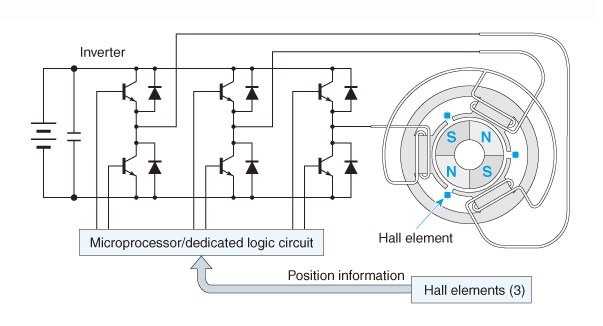
\includegraphics[width=\textwidth]{Motors/BLDC1}

A l'etapa de potència trobem un esquema molt similar als onduladors trifàsics. El nostre objectiu no és crear un senyal sinusoïdal sinó controlar impulsos de corrent continu que enviem al motor. Tenim el triple pont i podem connecta la fase que vulguem a a + i negatiu. Mitjançant el controlador disposem de 3 sensors opcionals d'efecte hall i el controlador hauria de ser capaç de mesurar la tensió de cada fase i la seva intensitat. Aquests controladors poden operar a diferents tensions i normalment treballen per tal de tirar el corrent generat al frenar el motor o a un activador per activar el corrent cap al sistema de control.
%en la eptapa de potenci trobem un esquema molt sismilar als onduladors trifacs dels motors de corrent altern, pero en aquet cas el nostre obgetiu no es crear una seudosinisuidal sino controlar els inpulsos de coorent continu que enviem al motor. tenim el triple pont i poden conectar la fase que volgem a a + i negetiu mitgenen el controlador disposem 3 sesors opcionas del efecta hall, i el controlador auria de ser capas de mesurar la tencio de cada fase i la seva intencitat. aquets controladors poden operar a difarentes tencions i normalemnt treballan amb grans intencitats, alguns del controladors apart disposens de una resistencia de descarga per tal de tirar el corrent de generat al frenar el motor o a un activador per activar el coorent cap el sistema de control,

\subsubsection{Oscil·lació de las fases}

En el cas de disposar de motors amb sensors d'efecte hall tindrem un punts de referència per saber en quin punt podem commutar les fases per obtenir la màxima eficiència i potència del motor. En canvi si el sistema de control el fem pel voltatge de la fase flotant estem pendents de la fase flotant per tal de saber en quin punt cal commutar les fases per que segueixi girant el motor.
%en el cas de diposer motors amb sensconrs de efecta hall tindrem un puts de per sapiger en quin punt podem comutar les fases por obtenir la maima eficencia i potencia del motor, en cavi si el sistema de control el fem per el voltage de la fase flotant estem pandets de la fase flotant per tal de sapiger en quin punt en de comuntar les fases per fer segi giratn el motor 

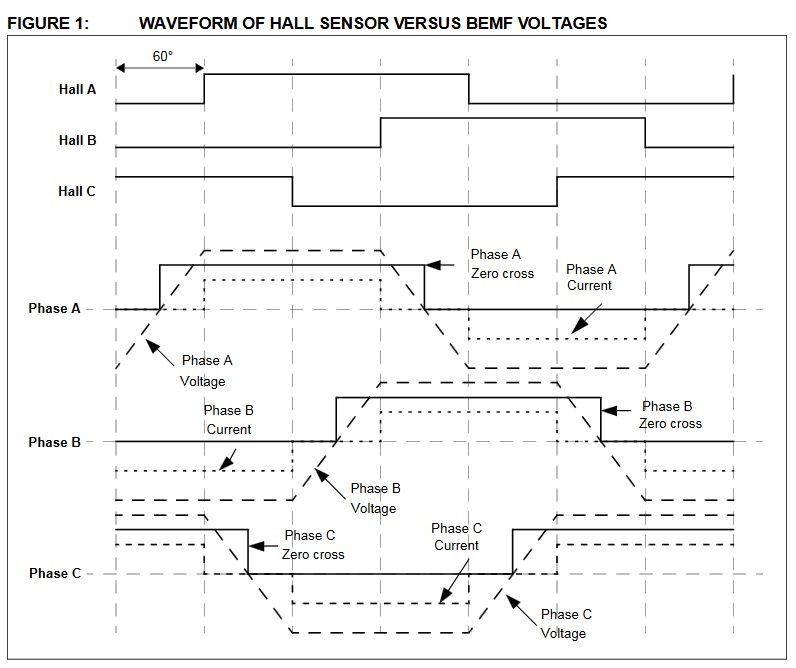
\includegraphics[width=\textwidth]{Motors/BLDC_DC_Motor_Sensorless_Trapezoidal_waveform}

En la part superior tenim els pins on el sensors d'efecte hall oscil·len determinant-se la forma del camp magnètic que tenim amb el rotor, per tal de conèixer la seva posició i saber quan commutar les bobines.

En canvi en els motors Sensorless hem de controlar el voltatge de la fase que penja, és a dir, quan estem alimentant les fases AB, la fase C queda lliure per poder capturar el voltatge i saber quan passa per 0 per activar la commutació. En el pas per 0 del voltatge de la fase voladissa per tal de detectar el canvi i coordinar la commutació.

Com es pot veure, els dos controlen la freqüència de commutació per fer accelerar el motor, ja que la velocitat d'aquests motors no es controla per la freqüència de gir, sinó pel voltatge de les fases. El control de la velocitat és el mateix que un motor de corrent continu amb escombretes depenent del voltatge de les seves fases, per això els transistors de l'etapa de potència els controlem amb un senyal PWM que defineix la velocitat del motor. En algunes aplicacions podria ser interessant calcular les revolucions a les quals gira el motor per fer-lo de llaç tancat. Per aquest tipus de motor no tendeix a trigar per aplicar càrrega sinó que demana un comú més alt d'amperes per tal de mantenir la velocitat amb molt poc o quasi nul amorrament, sempre que puguem gestionar la potència.
%com es pot veura com dels dos controla la frecuenci ade comutacio per fer acelarar el motor ja que la velositat de aquets motors no es controla per la frequencia de gir si no per el voltage de las pfases que saplien es a dir el control de la velositat es el matex que un motor deo corrent continu amb escoveta depedndre del voltage de las sevas fases, per aixo els trasistors de la etapa de potencia els controlaem amb PWm per definir la velositat del motr, en algunes paplicacion podria ser interantant calcular les rom del gira el motor per ferlo de llas tancat per aquet tipus de motor no tendex a amorarse al plicar carga sino que demana un comun mes alt de ambpers per tal de mentarni la velociat amb molt poc o casi null ammorrament sempre que pugem gestionar la potencia. 

\subsubsection{CPU de control}

Existeixen múltiples maneres de controlar un motor brushless. Cada marca té la seva pròpia manera de controlar-ho i tenen petites variacions, encara que totes tendeixen a una idea principal de control. En el cas en el que ens basem es mostra un diagrama de blocs d'una versió comercial de Texas Instruments.

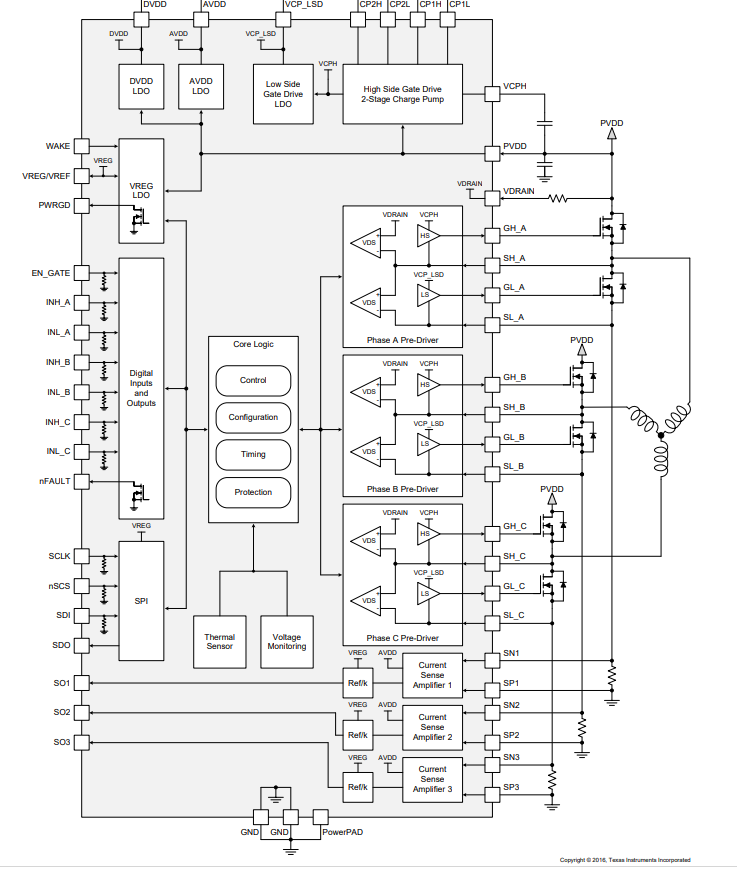
\includegraphics[width=\textwidth]{Motors/controlsquematic}

\textbf{Control dels transistors mosfet}\newline \smallskip

Si ens mirem els GH-A a sh-a, gl-a i sl-a controla una branca de l'inversor trifàsic que es composa de dos mosfets. Del motor tenim l'entrada sh-a i sl-a que estan connectades poder elevar la tensió de forma que el mosfet pugui obrir l'entrada de control, de forma que la tensió entre el gh-a i el sh-a es mantingui per sobre, suficient per mantenir el mosfet obert i controlar que tinguem curctcircuit. Per això mesurem la tensió entrel VDRAIN i el sh-a i comprovem la caiguda de tensió, de ser molt elevada tallem. També incorpora una mesura de corrent per fase, en la part inferior tenim el sn1, sp1 amb un shun per determinar la caiguda de tensió i saber la intensitat que circula per cada base.
%si ens mirem els GH-A sh-a gl-a sl-a controla una braca del inversor trifasic que es composa de dos mosfets de el motor tenim la intrada sh-a i sl-a que estan conectades per poder elevar la tencio de forma que el mosfet pugi obrir la entrada de cotnrol de forma que la tencia entre el gh-a i el sh-a es mentigi per sobre lo sufent per mentenir el mosfet obert i contolar que no tignem un corcirquit, per aixo mesurem la tencio entre el VDRAIN i el sh-a i comprovem la caiguda de tencio si es mol elevada tallem. tambe incormpera una mesura de corrent per fase, en la part inferor tenim el sn1 sp1 amb un shun per determinar la caguda de tencio i saver la intencitat que cirlula per cada fase. 

\textbf{Voltatges i fonts aïllades} \newline \smallskip

Per poder obrir el mosfet necessitem donar una tensió entre la gate i el source determinada per la conducció del mosfet. Hem de disposar d'una font de més voltatge que la font de la bateria principal, això ens provoca que s'hagin de fer fonts flotants per poder contrlar els mosfets. Això ja ho fa internament el controlador, però algunes tècnices serien carregar un condensador connectat entre el gate i el source i descarregar-ho per obrir el mosfet sempre que el temps d'obertura sigui petit i no descarreguem el condensador. A part hem de controlar la intensitat que necessiten els mosfets per forçar un tret ràpid, arribant a ser de 2A més o menys, i la mateixa en negatiu. En la part superior poden observar-se els condensadors que es fan servir per la porta d'alta i la font de conversió.

%per poder obrir el mosfet nesesitem donat una tesio entre la gete i el souce determinada per en conducio el mosfets de Higs em de disposatr de una font de mes voltage que la font de la bateria prisipal, aixo ens proboca que agem de fer fonts folotans per poder controlar els mosfets axo ga en ho fa internamen el contorlador pero algunes tecnices seria caregant un condensador que esta conecttat entre la surce i la gate i descagarlo per obrir el mosfet senpre que el tems de obertura segi petit i no descargem el condesador, apat emb de ocntolar la intacitat que domes els mofets per forcar un dispar rapid poden der de 2A mes o menso i la matexa en negatiu, en la part superior oden oberser els dos condesadors que es fan servir per la porta de alta, i la font de conversio\bigskip

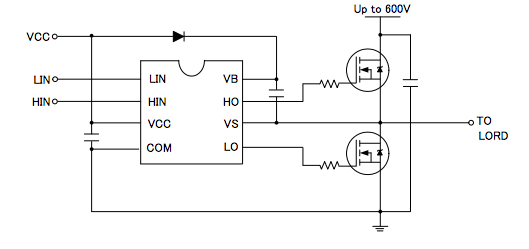
\includegraphics[width=\textwidth]{Motors/600-V-HighLow-Side-Gate-Driver-1427853331}

Aquí podem veure una mica aquest tipus de font. Ens centrarem en el VB, HO i VS que són la part interessant, ja que treballen per sobre del voltatge de HIGH voltatge. En estat de repós el H0 està connectat a massa i el corrent pot fluir des de Vcc fins a VS, de forma que el condenasdor queda carregat. Quan activem el tret del mosfet, el VB es connecta amb el HO de forma que tenim la tensió de la font en la porta del mosfet. Això provoca el tret del transistor i ens permet activar la porta i començar a conduir. Al conduir VS s'eleva per sobre VCC elevant el voltatge del condensador fins que el díode talli i ens quedi una font de VCC en el condensador per sobre la tensió del drenador del mosfet mantenint-lo obert. Al tancar-ho, el que fem és connectar-ho a massa i el díode i la font tornen a carregar el condensador per tornar-ho a tenir preparat. La resistència de la porta és perquè el condensador no es descarregui massa ràpid, arribant a cremar el mosfet limitant el corrent de la gate.
%aqui podem veura una mica quets tipus de font, ens centrerem el el VB HO VS qu son la pet interanet ga que trevalles per sobre del voltage de higvoltag, en estat de repos el H0 esta conectat a massa i el corrent pot fluit desde el vcc fins al vs de forma que el condesador queda carregat, cuan activem el dipsar el vb es connecta amb el HO de forma eu tenim la tencio de la font en la porta del mosfet aixo proboca el dipar del transistor i ens parment activar la porta i comensar a conduir, al cunduir vs saleva per sobre vcc elevant el voltage del condesador i fine que el diodi talli i ens queda una font de VCC en el condesador per sobre la tensio del drenador del mosfet manteninlo obert, al tancarlo el que fem es connectart Ho a masa i el diode i la font tornen a carregar el condesador per tornarlo a tenir preparar. la resitecia de la porta es per que elk condesador no es descare masa rapid poden cremar el mosfet limitat la corrent de la gate
 
 \textbf{Mètodes de control}\newline \smallskip
 
 Aquí si és on hi ha una àmplia diversitat entre marques i models, des de diferents interfícies de control, fins a disponibilitat d'entrades digitals, analògiques, PWM o comunicacions com CAN, SPI o Serial entre moltes més. Poden ser tant diversos que ens hem de mirar un producte en concret per saber com s'han de controlar. També disposen d'una unitat de processament per a les entrades corresponents o les comunicacions per tal de controlar tots aquests elements i  fer girar el motor com s'espera. 
 % aqui si que tenim un molt molt divers esntre marques i models comentails son la intefaces de control dels alemnts poden diposar de entredas digitals, analogicas pwm o mcomunicaicons com can, spi o serial entre moltes mes, poden ser tan diversos que ens em de mira run producte en conecnte per saver com san de controlar inclun estre marcas poden ser molt diverses,  tambe diposem de una unitat de prosesement CPU per amb les entrades correnspoents o les comunicacions controlar tots aquets elements i fer girar el motor com saspera. 
 
 \textbf{Característiques extres}
 
 Alguns controladors porten algunes característiques que poden ser interessant, com el control de l'alimentació de HV. Alguns ens permeten muntar un relé transistor per activar el HV. Podria ser interessant per no tenir tot el temps el circuit de potència connectat al motor. També alguns disposen d'una sortida per una resistència de crema, és a dir, en el cas que utilitzem el motor per frenar generarà una intensitat de sortida cap al HV. Si no la volem gestionar, és pot activar una resistència que actuï com a dissipador. També controlar la intensitat d'entrada al convertidor i controlar les resistències per tal de no injectar corrent al HV, entre altres funcions interessants. 

 \section{Elecció del motor brushless per al CVE}

Em decanto pels motors brushless pel prototip del controlador de vehicles elèctrics que tenim pensat implementar de forma teòrica. Els principals avantatges que ens donen aquest tipus de motor es llisten seguidament:

\begin{itemize}
    \item Major nombre de RPM, ja que no existeix pràcticament fregament. No disposen do commutació interna i només ens limitaria la commutació electrònica i el disseny mecànic del propi motor.
    \item No disposa de bobinat en l'interior del motor ni escombretes que provoquin fregament arribant a eficiències molt altes per sobre del 90\%. Això provoca que pràcticament no dissipen energia en forma de calor, donant una major autonomia de la bateria i menor desgast al no estar sotmès a altes temperatures.
    \item Major potència ja que no hem de crear els imants en el centre i amb uns imants permanent molt potents podem aconseguir entregues de potència molt altes, amb un pes molt baix com per exemple el Turnigy RotoMax 150cc Size Brushless que amb un pes de 2,3Kg aconsegueix una potència de 9,8Kw.
    %magor potencia ja que no em de crear els imans en el centre i amb uns impans permantats molt potens podem acosegir entregas de potencia molt altes amb un pes molt baix com peratgemple el Turnigy RotoMax 150cc Size Brushless  que amb un pes de 2,3kg aconsegim una potencia de 9,8 kw 
    \item Voltatges d'accionament reduïts. No en tots els casos, però per norma general aquests motors treballaran per sota els 60V. Això ens facilitarà el disseny d'una bateria es facilitarà el treball amb l'alt voltatge ja que estarem parlant de valors de 400V com en els d'alterna.
\end{itemize}

Tots aquests paràmetre ens porten a seleccionar aquest tipus de motor per al disseny del nostre controlador. Tot i que amb aquest tipus de motor la part més complex és el ESC que serà l'encarregat de controlar l'excitació dels camps de maneig per provocar el gir del motor. Tindrem avantatges extres ja que són un tipus de motor que molt fàcilment els podem convertir en generadors i tenint una eficiència alta podrem aprofitar per la frenada regenerativa per tal d'intentar millorar l'eficiència del VE. 




%%%%%%%%%%%%%%%%%%%%%%%%%%%%%%%%%%%%%%%%%%%%%%%%%%%%%%%%%%%%%%%%%%%%%%%%%%%%%%




% A PARTIR DE AQUI TODO MOVIDO AL VESC!!!!!!



%%%%%%%%%%%%%%%%%%%%%%%%%%%%%%%%%%%%%%%%%%%%%%%%%%%%%%%%%%%%%%%%%%%%%%%%%%%%%


\chapter{VESC}
\label{chap:VESC}

%\section{Funcions del VESC}

El vesc en un projecte d'opensofware i openhardware que en permet tenir un controlador de motor brushless dissenyat per a patinets elèctrics, el que ens és perfecte per controlar un motor per la nostra aplicació, a part en donar l'opció d'analitzar-lo internament

\section{Funcions del microcontrolador del VESC}

El microcontrolador tindrà emmagatzemades una sèrie de paràmetres per establir la configuració de funcionament sobre el motor, a més de paràmetres que també controlen la bateria. També disposa de diverses formes d'entrades per indicar paràmetre com el gas, sentit o extreure informació. La seva tasca és, donades les entrades designades com el gas i el sentit, determinar quins són els transistors i a quina freqüència cal generar la PWM  per tal de controlar el motor amb la màxima eficiència i generar el moviment, respectant els límits de temperatura, intensitat i voltatges tant del motor com de la bateria. 
% ??? QUIENTIO? BRUNET
%el micontrolador tinda etmagasandes una seria de paramentres del motor en quientio que podrem configurar amb la seva eina i tot de paramnes de control de la baterya. tembe disposa de vaires forma de entradas per indicar parametres com el gas sentit o extreura informacio, la seva tasca es donades les entrades designades com el gas i sentit, determinar quins transistors i a quina frequencia genera la pwm per tal de controlar el motor amb la maxima eficacia i generar el moviment, tot i respactant limits de temperatura intencitat i voltages tan del motor com de la baterya per fero de la foma mes segura 
    
\subsection{Control de la intensitat}

Un dels paràmetres principals a controlar és la intensitat. La intensitat és el factor que si es surt dels paràmetres adients pot provocar problemes en cremar components. Controlarem la intensitat mitjançant el control PWM de cada un dels transistors i mesurant la intensitat de cada fase per tal de no passar corrent en cap d'elles. A part porta intensitat màxima de drenatge de la bateria per tal de no superar els límits de la mateixa i per separat el controli intensitat màxima que pot extreure del motor cap a la bateria, per tal de mantenir el control del corrent en límits segurs. Això és degut a que les bateries tenen una capacitat molt més gran de donar corrent que de recuperar-la, a part de tot d'harmònics que poden aparèixer i pujada de voltatge en la bateria, donant-se una falsa sensació de tenir més bateria del compte. Aquest paràmetre ens permet regular-ho segons el voltatge de la bateria. Per exemple només donar corrent quan la bateria es troba més baixa d'un valor X o no donar més de XA per sobre de X.
%un del sparamentres prisiplas a controlar ja que es el que proba la magor part dels problemas de cremar els components. controlarem la intencitat mitgensant el control pwm de cada un dels mosfet i mesuran la intencitat de cada fase per tal de no pasasa de corrent en cap dellas, apat porte intencitat maxima de drenatge de la baterya per tal de no suparar els limits de la mateixa i per saparat el controli intencitat maxima que pot extreure del motor cap a la baterya per tal de mantanir el contol de la coorent en limits segus. axo es debut a que les bateryas tenen un capcasitat molt mes gran de donar corrent que de recuperarla apart de tot de ermoics que en poden apareixa i pugada de voltage en la baterya donanse una false sensacio de tenir mes baterya del conte, aqut paramente ens perment regularlo segons el voltage de la baterya per etgemple domes donnar corrent cune esta mes vaixa de X o no donan mes de XA per sobre de X, 
 
Tenir en compte que el control pot extreure corrent de la bateria emmagatzermar-la en els condensadors d'alimentació donant més intensitat al motor de la que pot extreure de la bateria durant petits períodes de temps. Per això és obligatori configurar el motor i la bateria en les intensitats corresponents, encara que siguin diferents.    
%teni en conte que el controlar pot extreure corrent de la bterya i emagamale en els condesadors de alimentacio donan mes intenciat el moto de la que pot extreure de la baterya durant pocs periodes de tems, per aixo es obligatori configurar el motor i la baterya en les intencitat corespoents. encara que sigin difarents. 
    
\subsection{Control de rampes}
En els motors elèctrics un dels principals inconvenients en el que ens trobem és que tenen un par de força pràcticament instantani. Això ens pot donar una experiència de conducció brusca i incòmoda. Per això el microcontrolador el que fa és definir un temps progressiu d 'arrancada i frenada per arribar al valor determinat. Quan més gran sigui el temps més trigarà a aconseguir la potència requerida i la conducció es farà més suau. Conforme baixi aquest temps, la conducció serà més agressiva. 
%en els motorn electric un dels inconvients que en trobem en el notre cas es que tenean un par force practicament instantani i axo ens pot doner una experiencia de conducio brusca e incomode. per axo el micocontroldor el que fa es defienir un tems progresis de arencada i frenada per arivar el valor detarmintat cuan mes gran es el tem mes tardara a consegir la poencia requeria i la conducio es fara mes suau i cuent meson tems mes \newline agresiva sera la conducio \bigskip

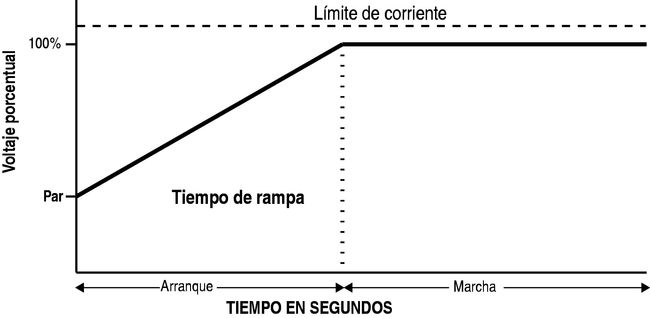
\includegraphics[width=\textwidth]{rampa}

Això es pot complicar empalmant múltiples rampes per RPM permetent oferir una corba de potència per millorar l'eficàcia del motor i la seva autonomia. Es basa en determinar unes potències a unes determinades revolucions i poder adaptar com vulguem la corba de potència.

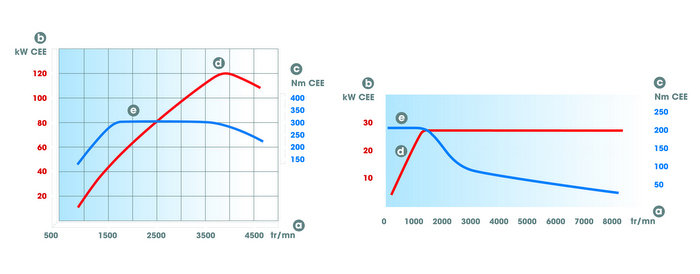
\includegraphics[width=\textwidth]{Motors/curves}

La corba de potència típica d'un motor de combustió dièsel i un motor elèctric, el disposar d'una corba tan plana ens permet jugar amb aquestes variables per tal d'emprar el par més eficient del motor i millorar l'eficiència general del vehicle, de forma que anem a buscar la corba d'un dièsel en la part eficient del nostre motor o busquem algun altra característica desitjada. En el cas de la frenada regenerativa també podem programar una corba de la intensitat que volem prenar per RPM i així millorar l'experiència de conducció.
%corba de potencia tipica de un motor de explosio disel i un motor elecric, el diposar de una corba tan plana podem gugar amb aquetas veirables per tal de utilisar la par mes eficent del motor i millorar el eficencia genaral del veicle de forma que anem a bucar la corva de un diesel en la part aficent del nostre motor o busquem alguna altre caracteritica desitgada, en el can de les frenades regenerativa tambe podem programenr un corba de la intenciat que volem drenar per RPM i axi millorar la expereincia de conducio\bigskip

\subsection{Control de la potència i les revolucions}

Podem configurar el nombre de Watts que podem injectar al motor o d'amperes per fer treballar el motor en un rang determinat, podent-lo controlar per no sobrepassar-se de potència i cremar-ho. Igual que limitar la potència total del motor, aquests paràmetres són absoluts ja que després amb les corves de potència podem reajustar-ho. Aquests valors absoluts es consideren els màxims. Ajustant la freqüència, és a dir, les revolucions del camp elèctric que li enviem al motor per tal de limitar les revolucions del motor i no sobrepassar uns límits. Per defecte i construcció tenim un límit de 50KHz en aquest driver.
%podem configurar el nobre de wats que podem igectar el motor o de ampers per la de ferlo treballar en un rang determintat i poderlo controlar per no sbobrepasarnse de potencia i cremarlo, ijual que limitar la potencia total del motor, aquts paramentres son absuluts ja que depres amb les corves de potencia podem reagustalos i ens el podem pendre com a maxims, tambe podem agustar el nombre de Hz es a dir las rebolucions del camp electric que li enviem al motor per tal de limitar les rebolucions del motor i no sobreparar un limits, per defecta i contrucio tenim un limit de 50khz en aquest driver \smallskip

\subsection{Control de temperatures}

En tot vehicle elèctric els components que gestionen la potència dissipen un percentatge d'energia en calor, i cal tenir-ho en compte per a no sobreescalfar components. Tenim l'opció de muntar un sensor de temperatura en el motor i es controla igual que amb els sensors interns.
%en tot veicle electric els compnenets que gestionen la potencia en disipan part en forma de calor i sa de tenir en conte per no sobrecalantar components, tenimm la ocio de montar senseor de temperature en el motor i controlo ijual que fariem amb els interns,

El control de temperatura ens pèrmet definir unes temperatures llindar per tal d'activar o desactivar ventiladors com a primera mesura de control. Una vegada seguim pujant de temperatura ens apareix l'opció de rampes limitadores, és a dir, unes rampes que van de la potència màxima a 0 en funció dels graus del dispositiu o el motor, limitant el seu consum de potència i evitant que s'escalfi més. És a dir podem dir que el motor de 100º a 150º vagi baixant la potència de 50Kw a 0Kw, això voldrà dir que a 120º el motor tindrà un màxim de 30Kw.
%el control de temperatura en perment defirn unas temperatura llindar per tal de activar o desactivar ventiladors com a primera mesura de control. una vegada segim pugat de tempratura ens aparaex la ocio de rampes limitadores, es a dir una rampes que van de la potencia maxia a 0 en funcio del graus del dispitiu o el motor, limitant el seu consum de potencia i evitan que es calenti mes, es a dir podem dir que el motor de 100º a 150º vagi la seva poencia de 50kw a 0kw axo voldra dir que a 120º de motor  tindrem un maxim de 30kw al motor. 

\subsection{Control del FOC}
Funcionament en mode sinusoïdal del camp electromagnètic, és a dir, en comptes de commutar les bobines en PWM es simula una quadradad que oscil·la dacord amb les revolucions del motor i amb el voltatge del motor per la velocitat en qüestió. Ho fem amb una sinusoïdal oscil·lant a la mateixa freqüència i amb el mateix pic de control, això provoca que les 3 fases estiguin energitzades i no tinguem fase lliure per al control. Això vol dir que només està disponibles per a motors Sensored, a part la freqüència de commutació sòl ser fixa i no es permet reduir el nombre de commutacions dels mosfets. Dóna un control molt més complert de la direcció dels camps que estem generant i que el camp no oscil·li en forma de polsos al canviar les bobines. Algunes avantatges queden mostrades a continuació:
%funcionament en mode sinusiodal del camp electro magnetic, es a dir en vens de comutar las bobines en pwm simulan una cuadrada que olisa acord amb les rpm del motor i amb el voltage del motor per la la velocitat en cuestio, o fem amb una sinosudal osilan a la matexa frequencia i amb el matex pic de control axo proboca que les 3 fases estigin energisada s i no tingem fase lliure per el contorl, axo vol dir que domes esta diposnible per a motors sensored, apart la freqcuente de ocnmutacio sol ser fixa i no es parment reduir el nobre d ecomutacions dels mofets pero en dona un coltrol molt mes complert de la diracio del camps que estem generant i que el camp no osisli en forma de pulsos al camviar les bobines algunes vantages son:
\begin{itemize}
    \item Es necessita una mesura de la posició i velocitat del rotor.
    \item El par i el flux magnètic poden canviar ràpidament en menys de 5-10 mili-segons. 
    \item La resposta de cop tendeix al revessament si s'utilitza un múltiple de pi. 
    \item Freqüència de commutació constant.
    \item La precisió del par depèn dels paràmetres que tinguem en el motor i poden ser precisos o produir grans errors.
    \item Es requereix més control per part de la CPU.
\end{itemize}

És el millor sistema de control ja que fem servir tots els bobinats del motor. Podem canviar el par generat molt més ràpid i no sobrecarreguem dos bobines sinó que interactuen les 3 per tal de controlar el motor. Ens dóna una experiència de conducció molt més suau sobretot a baixes revolucions, però comporta problemes en la potència de càlcul necessària i l'obligació de sistemes de control extern, perdent eficàcia.

\subsection{Control de la freqüència del senyal PWM variable}
en algunts moments es molt iteresant reduir o aumentar la frequencia de comtunacio de la ona pwm per tal de enviar moltiseimis comutacions insesearies, es a dir si estem fen girar al motor a 10hz no es nesasari fer osilar el pwm a 50khz aixo probocari un consum exesiou en el fet de obrit i tancar el transistors a una velocitat exsasiva, per axo podem regular la frecuencia de comutacio de la pwm del motor, es un intent per millorar la suavitat i eficacia a baixa rebolucions.

\subsubsection{PID}
El microcontrolador també té un control PID per tal de controlar la velocitat, lo que vindria a ser el control de velocitat d'un cotxe. També disposa d'un control de la posició. És emprat en alguns PEV per mantenir la posició si no es dóna cap senyal, és a dir, que podríem deixar un skate o un patinet en una pendent i es mantindrien quiets si el PID està ben configurat.

\subsubsection{Mode d'entrada}
En el microcontrolador tenim el mode d'entrada d'ordre o sortida de dades, per tal de ser compatible amb els dispositius de mercat. Aquest model en concret seria per un senyal PWM i ADC com els més bàsics que controlen el gas que donem al motor, ja veurem que podem tenir diversos tipus de control.

Disposa de communicació serial per poder llegir informació i enviar ordres escrivint i llegint una sèrie de registres del microcontrolador, de forma que a part de controlar el gas podem llegir paràmetre com la intensitat, la potència consumida, entre d'altres.

També podem combinar diverses PWM o ADC i UART per poder llegir i treure informació per una banda i controlar per l'altre canal. Això podria ser útil per si volem disposar d'una interfície per llegir dades i el control posar-ho directament al driver per ADC o PWM. També tenim dos protocols més com el I2c i el NRF.
       
\subsubsection{Mètodes de control}
 Depenent del mètode per donar un gas determinat tenim diferents mètodes de control, és a dir, diferents formes de convertir aquest gas en la potència que donem al motor. Un d'ells i el més típic seria el control per corrent. A més gas més corrent, de forma que donem més potència al motor. El fet és convertir la variable PWM o ADC, en registre en corrent de forma que si es fa negativa invertim el sentit del corrent.
 
 La següent forma és corrent no invertida que seria molt similar sense poder fer girar el motor enrere i el wih break que seria sense frenada regenerativa per frenar. Després tenim el duty cycle que seria controlar el voltatge del pols del motor per tal de fer-ho accelerar sense tenir en compte la potència que demanem sempre sense passar-nos dels límits.
 
 Per acabar tenim els PID. Aquest controla la velocitat actual i en gestiona la potència del motor. 
 
 Si utilitzem el control per ADC tenim la peculiaritat que podem utilitzar dos controls; un per potència positiva i un per potència negativa, frenada o marxa enrere. Si utilitzem UART tenim els registres per fer la lectura i escriptura i amb NFR o el controlador de la consola Wii disposem del control de corrent que enviem cap el motor.
 %depenet de metoda per donar "gas" selecionat tenim diframents metodes de control, es d dir difarentes formes de convertir aget "gas" en la potencia que donem el motor, un dells i el mes tipic seria el control per corrent es a dir  ames gas mes corrent de forma que donem mes potencia el motor, el fet es convertir la pvariable OWM ADC; o valor en registre en coorent de forma que si es fa negativa invertim el sesntit del corrent. la segunet forma es currrent no reverse que seria molt similar sensa poder fer girar el motor enredera i el wih brake que seria sensa frenada regenetatiba per frenar, depres tenim el duty cicle que seria controlar el "voltage" del pol del motor per tal de ferlo acelerar sensa tenir en conte la potencia que denamem sempre sensa pasarnos del slimits\smallskip
 %per a acabar tenim els pid el que fareim eel gas i amb un PID controlar la velositat actual i na gestionan la potencia del motor.\smallskip 
 %si utilem el control per adc tenim la perticularitat que podem utilisar dos controls un per la potencia "positiva" i un per la potencia negetiba, frenada o marxa atras. si utilisem uart tenim els registres per fel la lectura i escriptura i amb nfr o wii (mando de la wii) donem dipsoem del el control de cootrent que enviaem cap el motor. 
      
\subsubsection{Analitzador de dades}
En aquest prototip tenim el control de dades, és a dir, el microcontrolador és capaç de fer un mostreig de les dades que tenim, com per exemple la intensitat, temperatura, potència, entre d'altres. Per poder-les enviar després per Serial o connectar-ho a un ordinador per analitzar les dades i decidir si cal fer alguna acció en aquestes dades. Al ser el propi microcontrolador qui enregistra les dades, si es volen llegir per la UART haurem de retirar dades constantment per tal de no saturar la memòria o mostrejar dades en poc temps.      
      
\section{Electrònica del VESC}
El projecte VESC trobat a Internet ja ens dóna els esquemàtics per a la seva implementació:

L'esquema més general es pot observar diferenciant els 3 blocs principals més alguns extres.
%en el esquema mes general podem observer que tenim el disposiu dividt en 3 blocks prisipals mes alguns extres.\smallskip
    
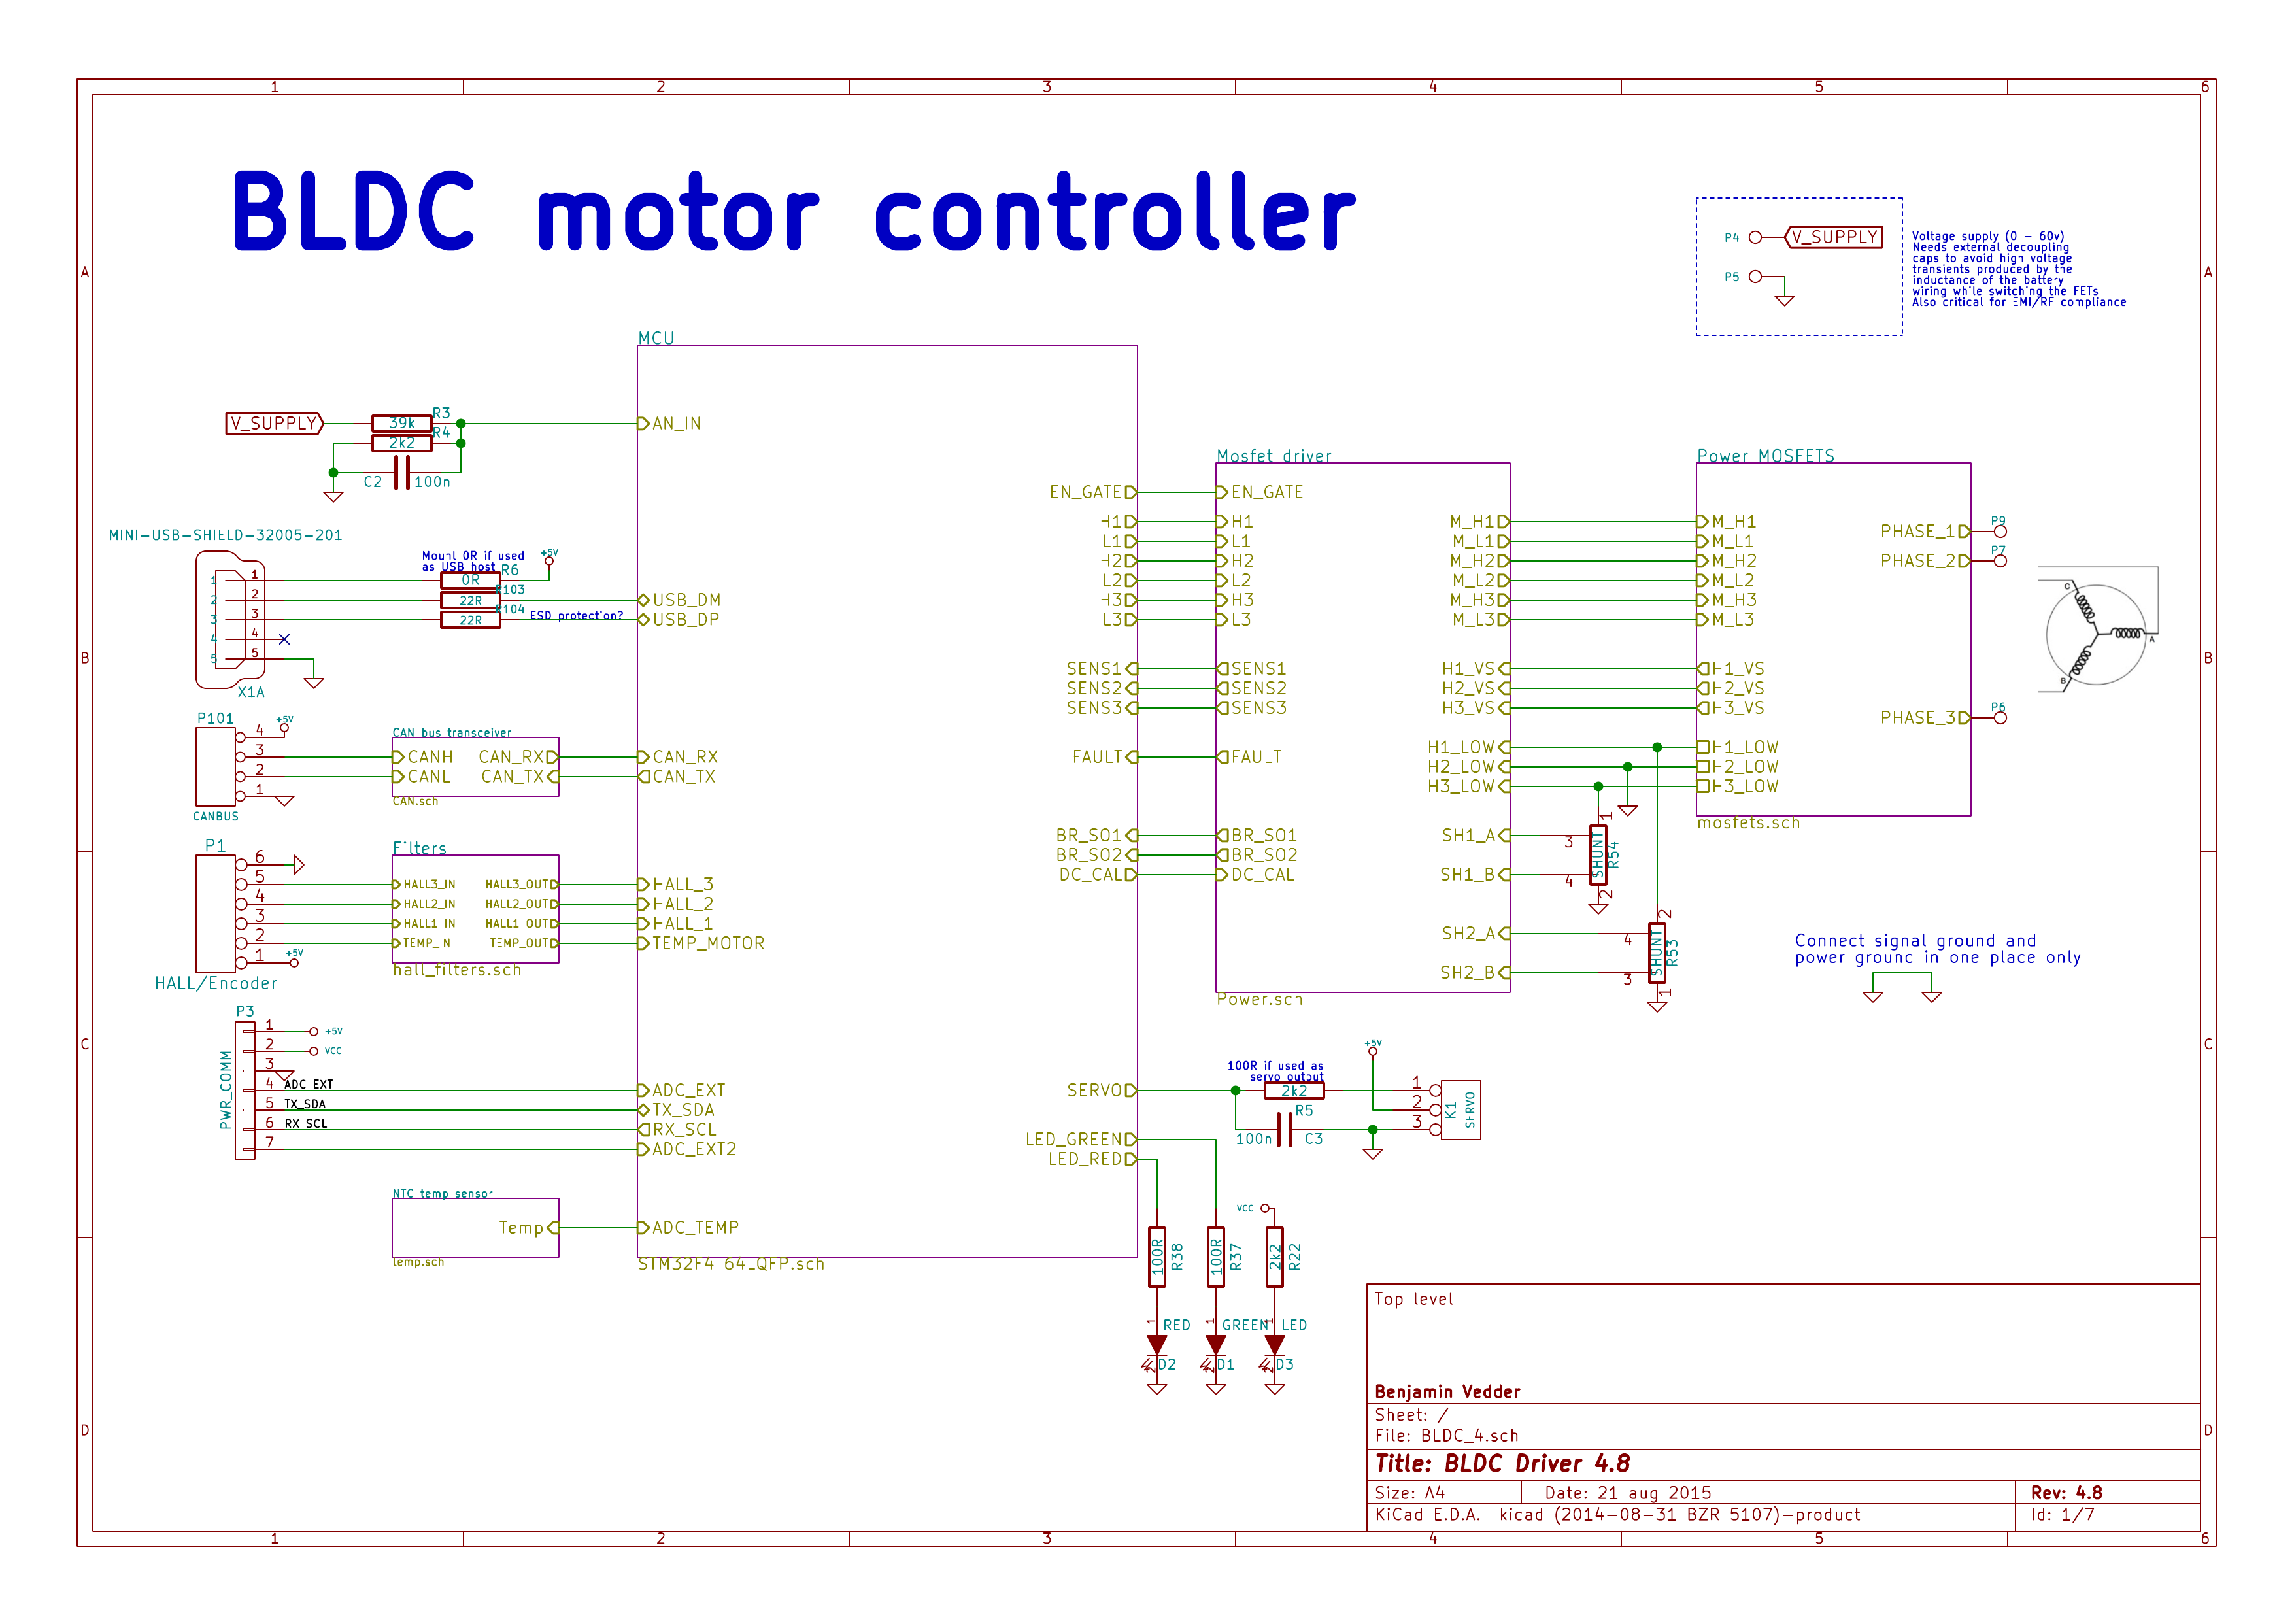
\includegraphics[width=\textwidth]{VESC/Schematic-1}
       
Podem observar que tenim el microcontrolador encapsulat amb el MCU i en el qual deriven senyals de diferents llocs. En aquests senyals depenent de com s'hagi configurat el firmware, es pot controlar el motor de diverses formes. Un cop hàgim realitzat els càlculs necessari passem el control dels mosfets de potència que rebran la informació del pont de transistors per activar o no les bobines necessàries.     
%podem oserver que tenim el micro encalusat amb el MCU i en el cual eriven senyasl de fiafrents llocs en quetes senyal depenent de com agem configura el frimware podem controlarlo el motor de difrentas formes, un coo agem realisat els calculs nasesaris pasem el control dels mosfets de potencia que rep informacio del pont de trensistors de trnesitors per activar o no les bonoines nesesaries
     
\subsection{Power mosfets}

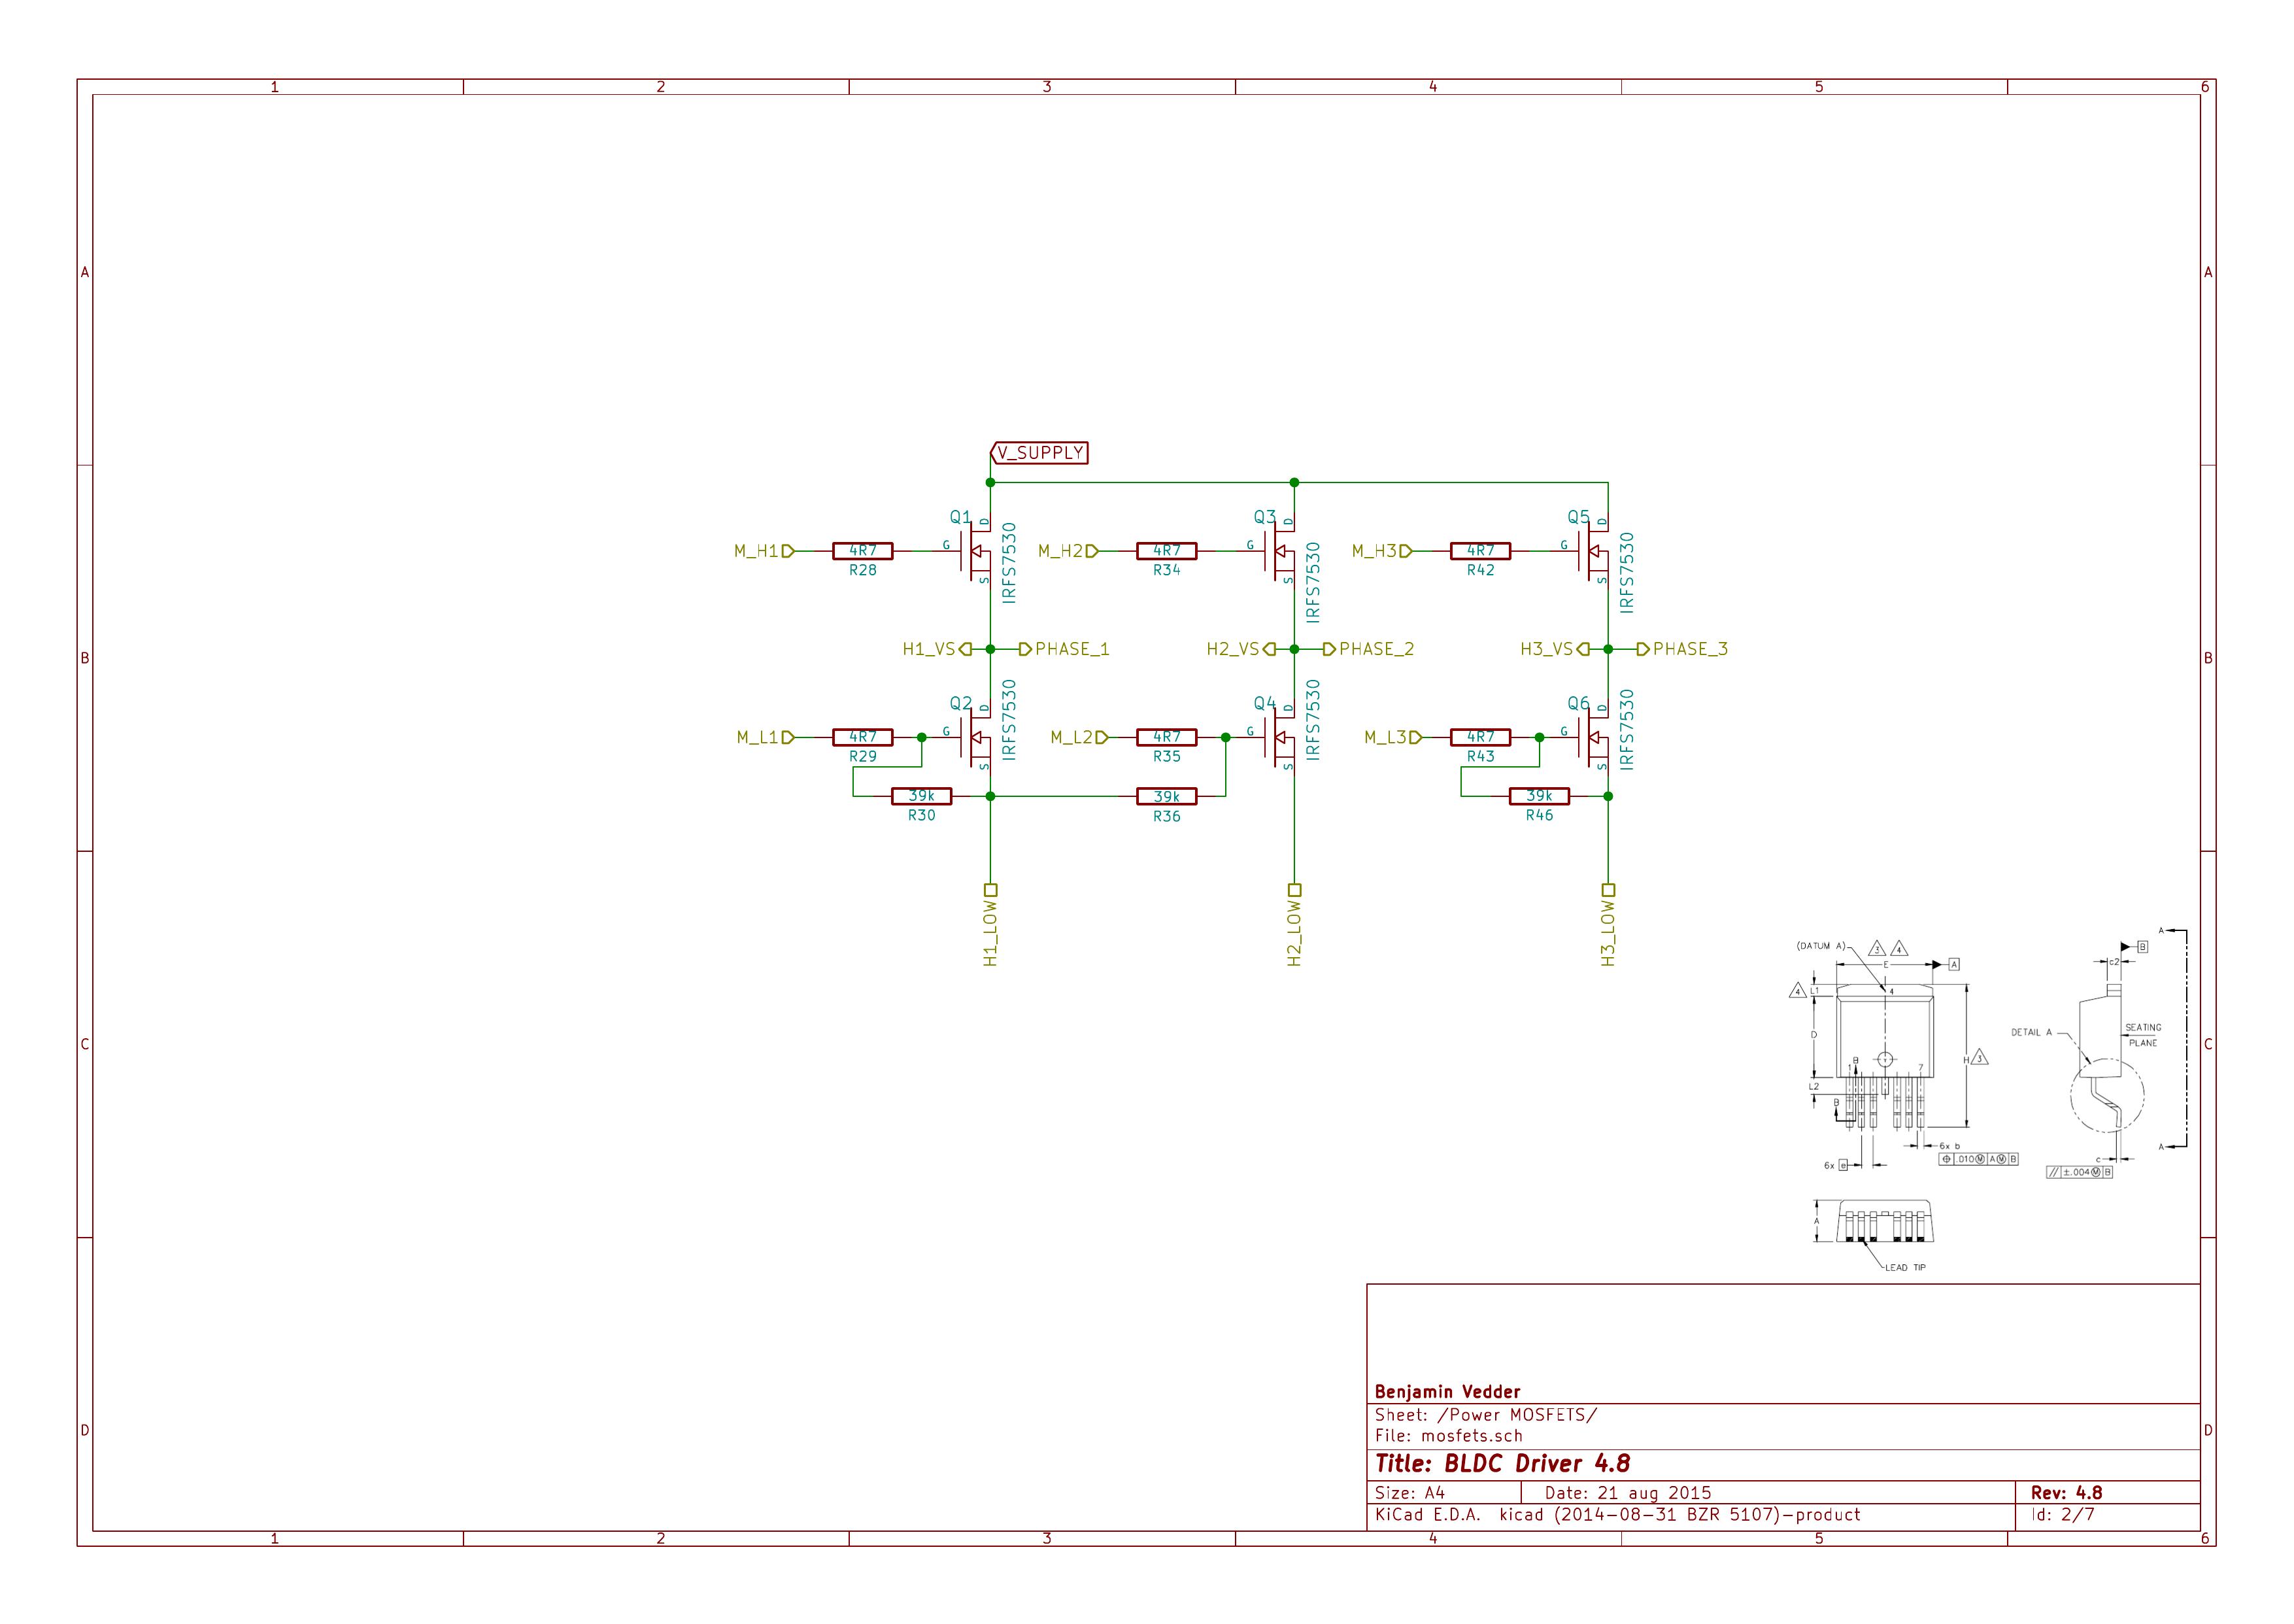
\includegraphics[width=\textwidth]{VESC/Schematic-2}
 
En la part dels mosfets tenim un triple pont en H per tal de poder generar les 3 fases que necessiten els motors brushless. També tenim els mesuradors de caiguda de voltatge en els mosfets per tal de poder detectar el curtcircuit en les diferents fases.
 
\subsubsection{Detecció de curtcircuit en l'inversor trifàsic}
 
 En un pont en H doble o triple si tenim el corrent que hi ha entre Vcc i el mig del pont. Podem detectar curtcircuits ja que el voltatge de caiguda que tindrem en el mosfet serà més elevat que el que tindríem si la potència passés per la bobina. Com sabem el mosfet proporciona un control resistiu, és a dir, podem canviar la seva resistència canviant la tensió entre la gate i el source. Això provoca un canvi de resistències entre el source i el drain. Sabent la tensió del source i la tensió del drain podem veure que tindríem una caiguda de tensió depenent de l'estat del mosfet. Si en la sortida hi hagués un curtcircuit, pràcticament tota la tensió es quedaria entre el source i el gate de forma que podem mesurar la intensitat de cada una d'elles. Podem observar unes resistències entre el gate i el source de forma que podem detectar-la i obrir el mosfet per no cremar-ho.
  
%\paragraph{detactar corciuquit en inversor trifaisc}
%en un pot en H doble o triple si tenim la corrent que hi ha entre el VCC i el mix del pont podem detactar corcirquits ja que el voltage de caijuda qur tindrem en el mosfet sera mes mes alavat que el que tindriam si la potencia pasa per la bobina, com saveme el mosfet proporciona un control resisitiu es a dir podem camviar la seva resistencia cavient la tensio entre el gate i el source, axo proboca un cavi de resistencia entre el source i el drain, si svem la tancio de la souce i la tencio del dran podem veure que tindrem una caiguda de tencio depeen del estat del mosfet, si en la surtida hi hages un corcicurut practiament tota la tencia escada entre el source i la gate de forma que podem detactarla i obrir el mosfet per no cremarlo.\smallskip 
     
També tenim les sortides de les branques separades per tal de poder mesurar la intensitat de cada una d'elles. Podem observar unes resistències entre la gate i el pin de tret per tal de limitar la intensitat que demanem al controlador.
%tambe tenim las sortides de las bracas separadas per tal de poder masurar la intenciat de cada una de ellas, podem obersar unses resisitecias entre ela gate i el pin de dispar per tal limitar la intencitat que demanem al controlador, 

\subsubsection{Intensitat del gate}
 En el gate d'un mosfet per norma general apareix un condensador. Això provoca que el tret del mosfet necessiti una intensitat per tal de carregar aquest condensador, si la intensitat no la limitéssim podríem cremar el control.
%\paragraph{intenciat en la gate} en las gsates del un mosfet per noma general aparex un capacitador aixo proboca que el dispar del el mosfet nenesisit una intenciatat per tal de carregar aquet capacitador si la intanciat que no la limitencim podriem crremar el control. 
     
\subsection{controlador del inversor}
En el VESC per dissenyar l'inversor trifàsic s'han basat en el xi DRV8302 per tal de controlar les 3 branques de pont en H:

\subsubsection{Descripció del DRV8302 }
L'integrat disposa d'unes entrades de control que permeten donar senyals als mosfets de potència per activar-los, de forma que ell eleva el voltatge i activa el mosfet. El mosfet ha d'estar a 5V entre gate i source, però el source en el moment de l'activació canvia de GND a VC menys la caiguda del mosfet. Si li apliquéssim 5V referenciats a massa no aconseguirem obrir el mosfet. Aquest integrat permet controlar tot aquest procés.

A part en permet capturar la mesura de corrent en dues de les fases, per tenir un control constant del corrent que fem circular pel motor i controlar el curtcircuit, just al moment en el qual el mosfet rep tota la caiguda de voltatge.

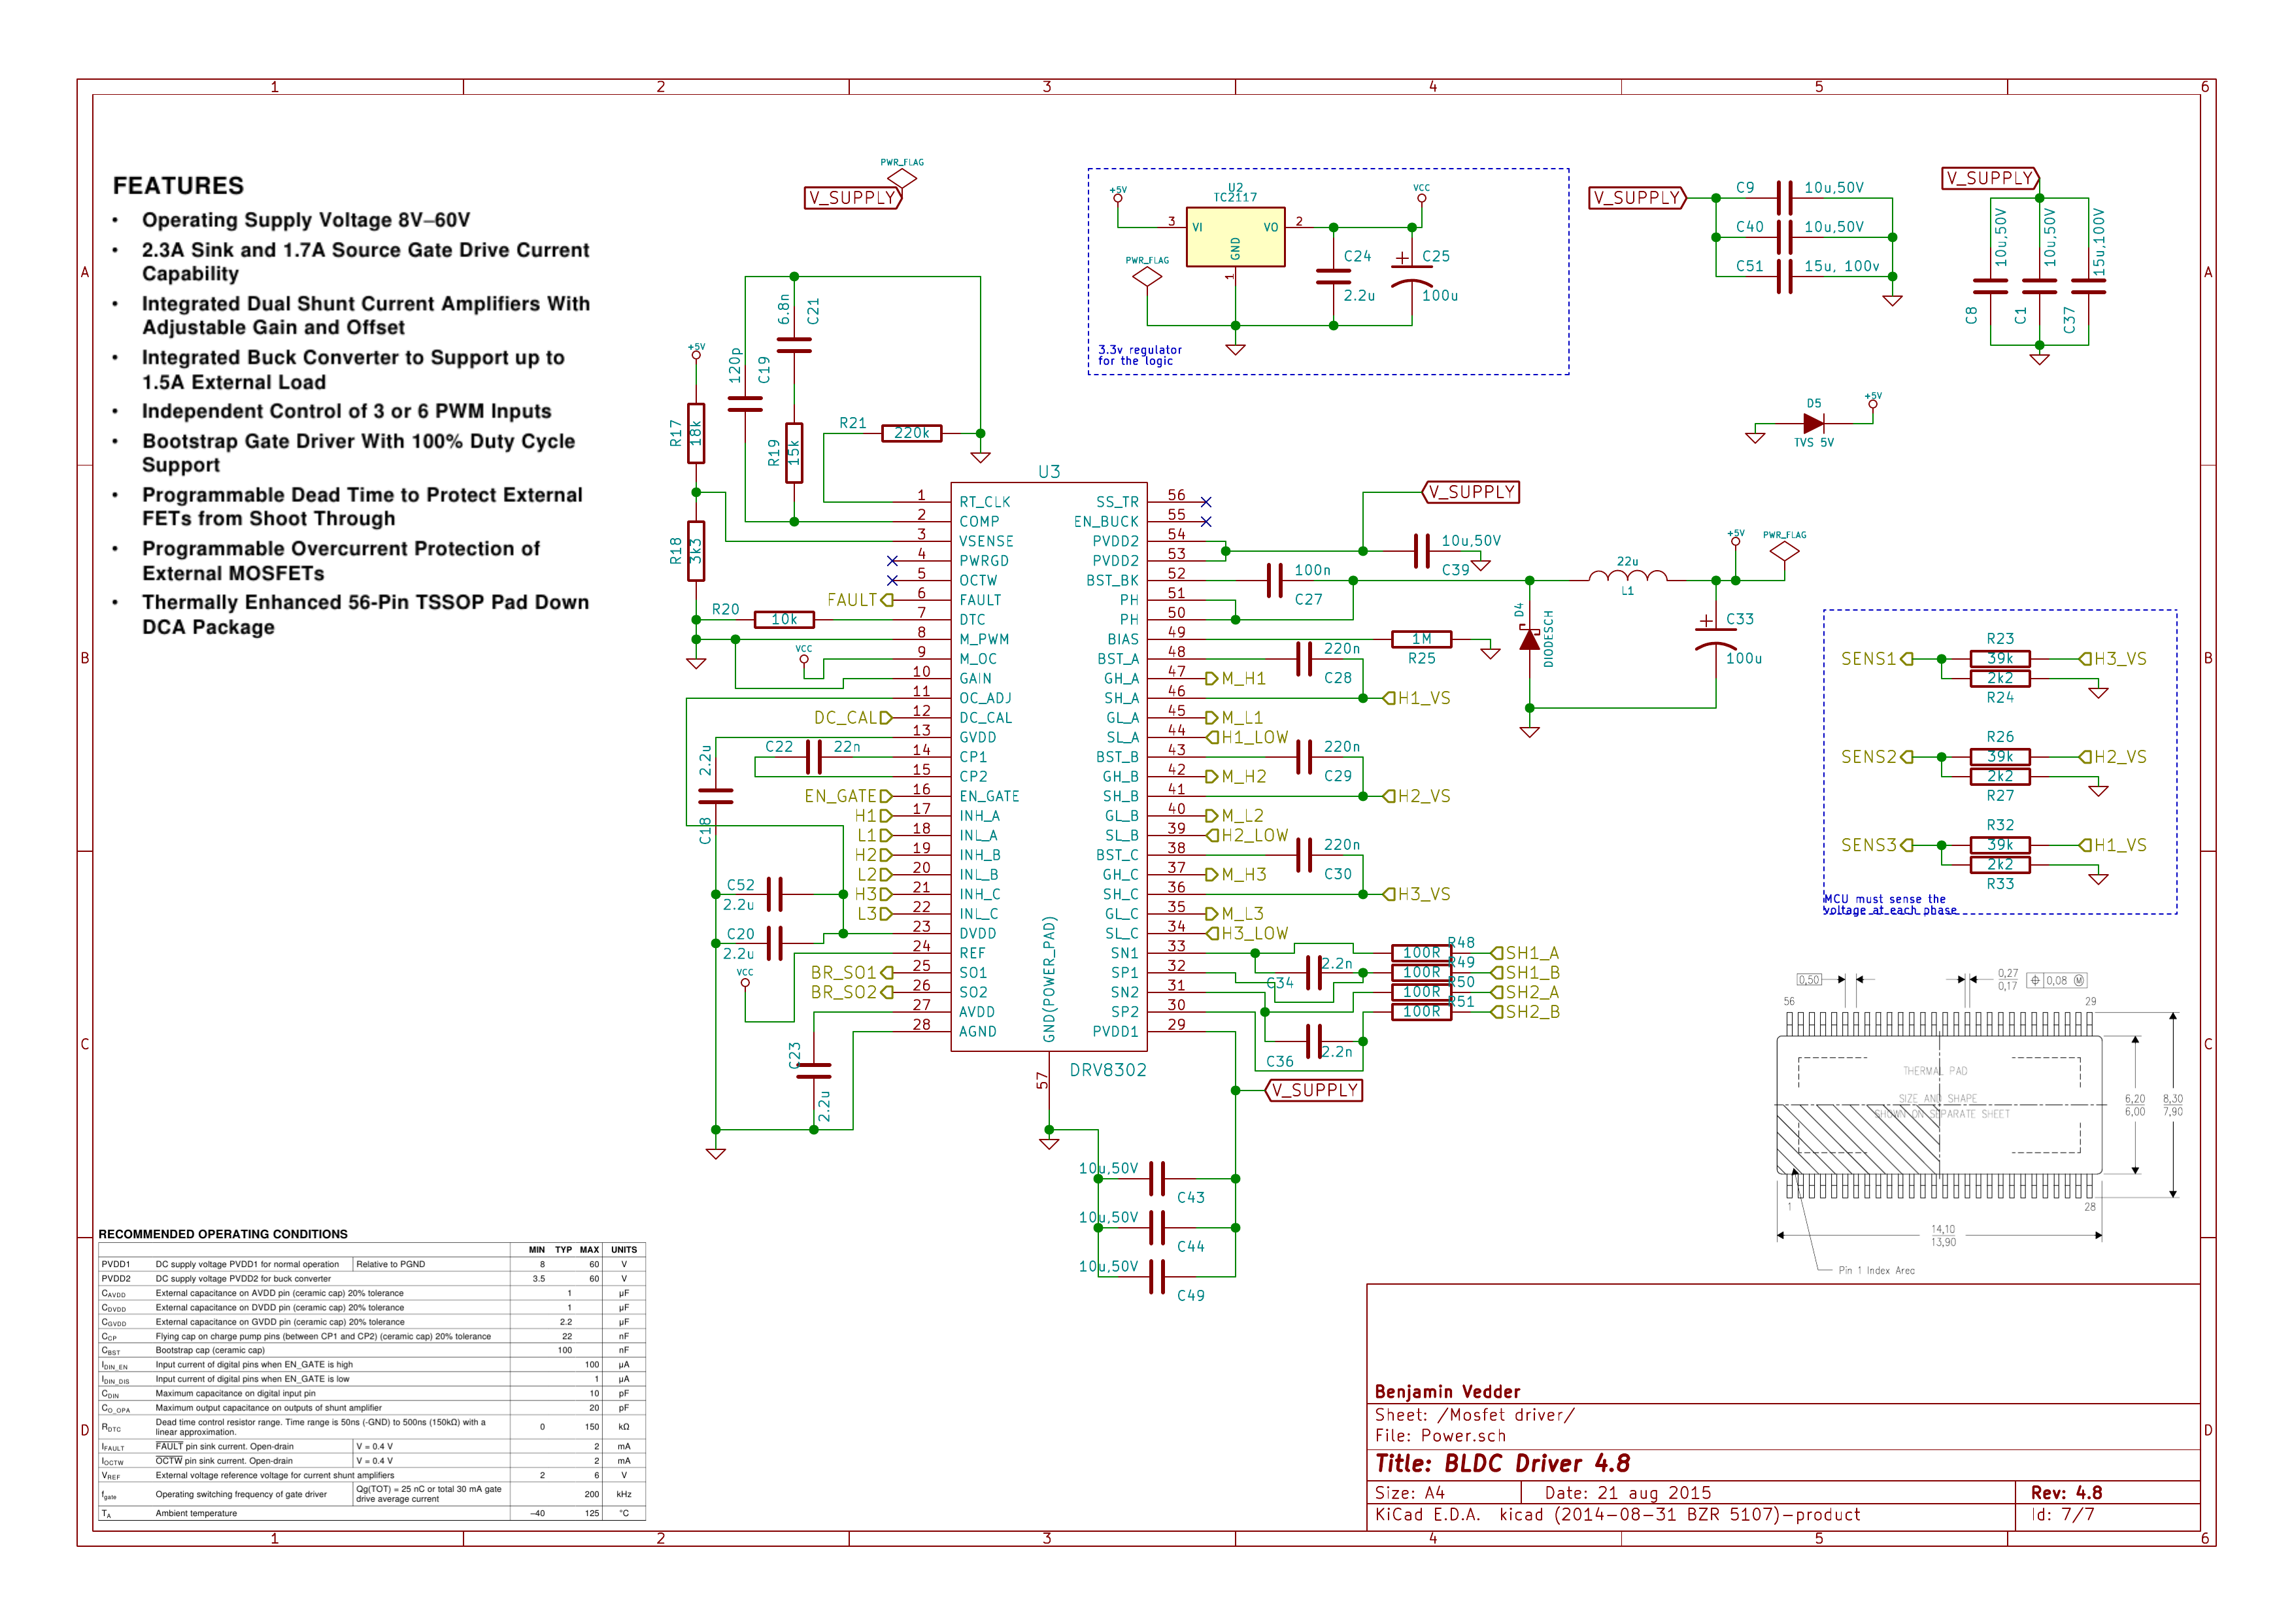
\includegraphics[width=\textwidth]{VESC/Schematic-7}

\subsection{Microcontrolador}
En el VESC disposem d'un microcontrolador capaç de controlar l'inversor trifàsic per tal d'adaptar-se a les característiques de software que tenim explicades. Aquest microcontrolador és un ARM CORTEX M4.

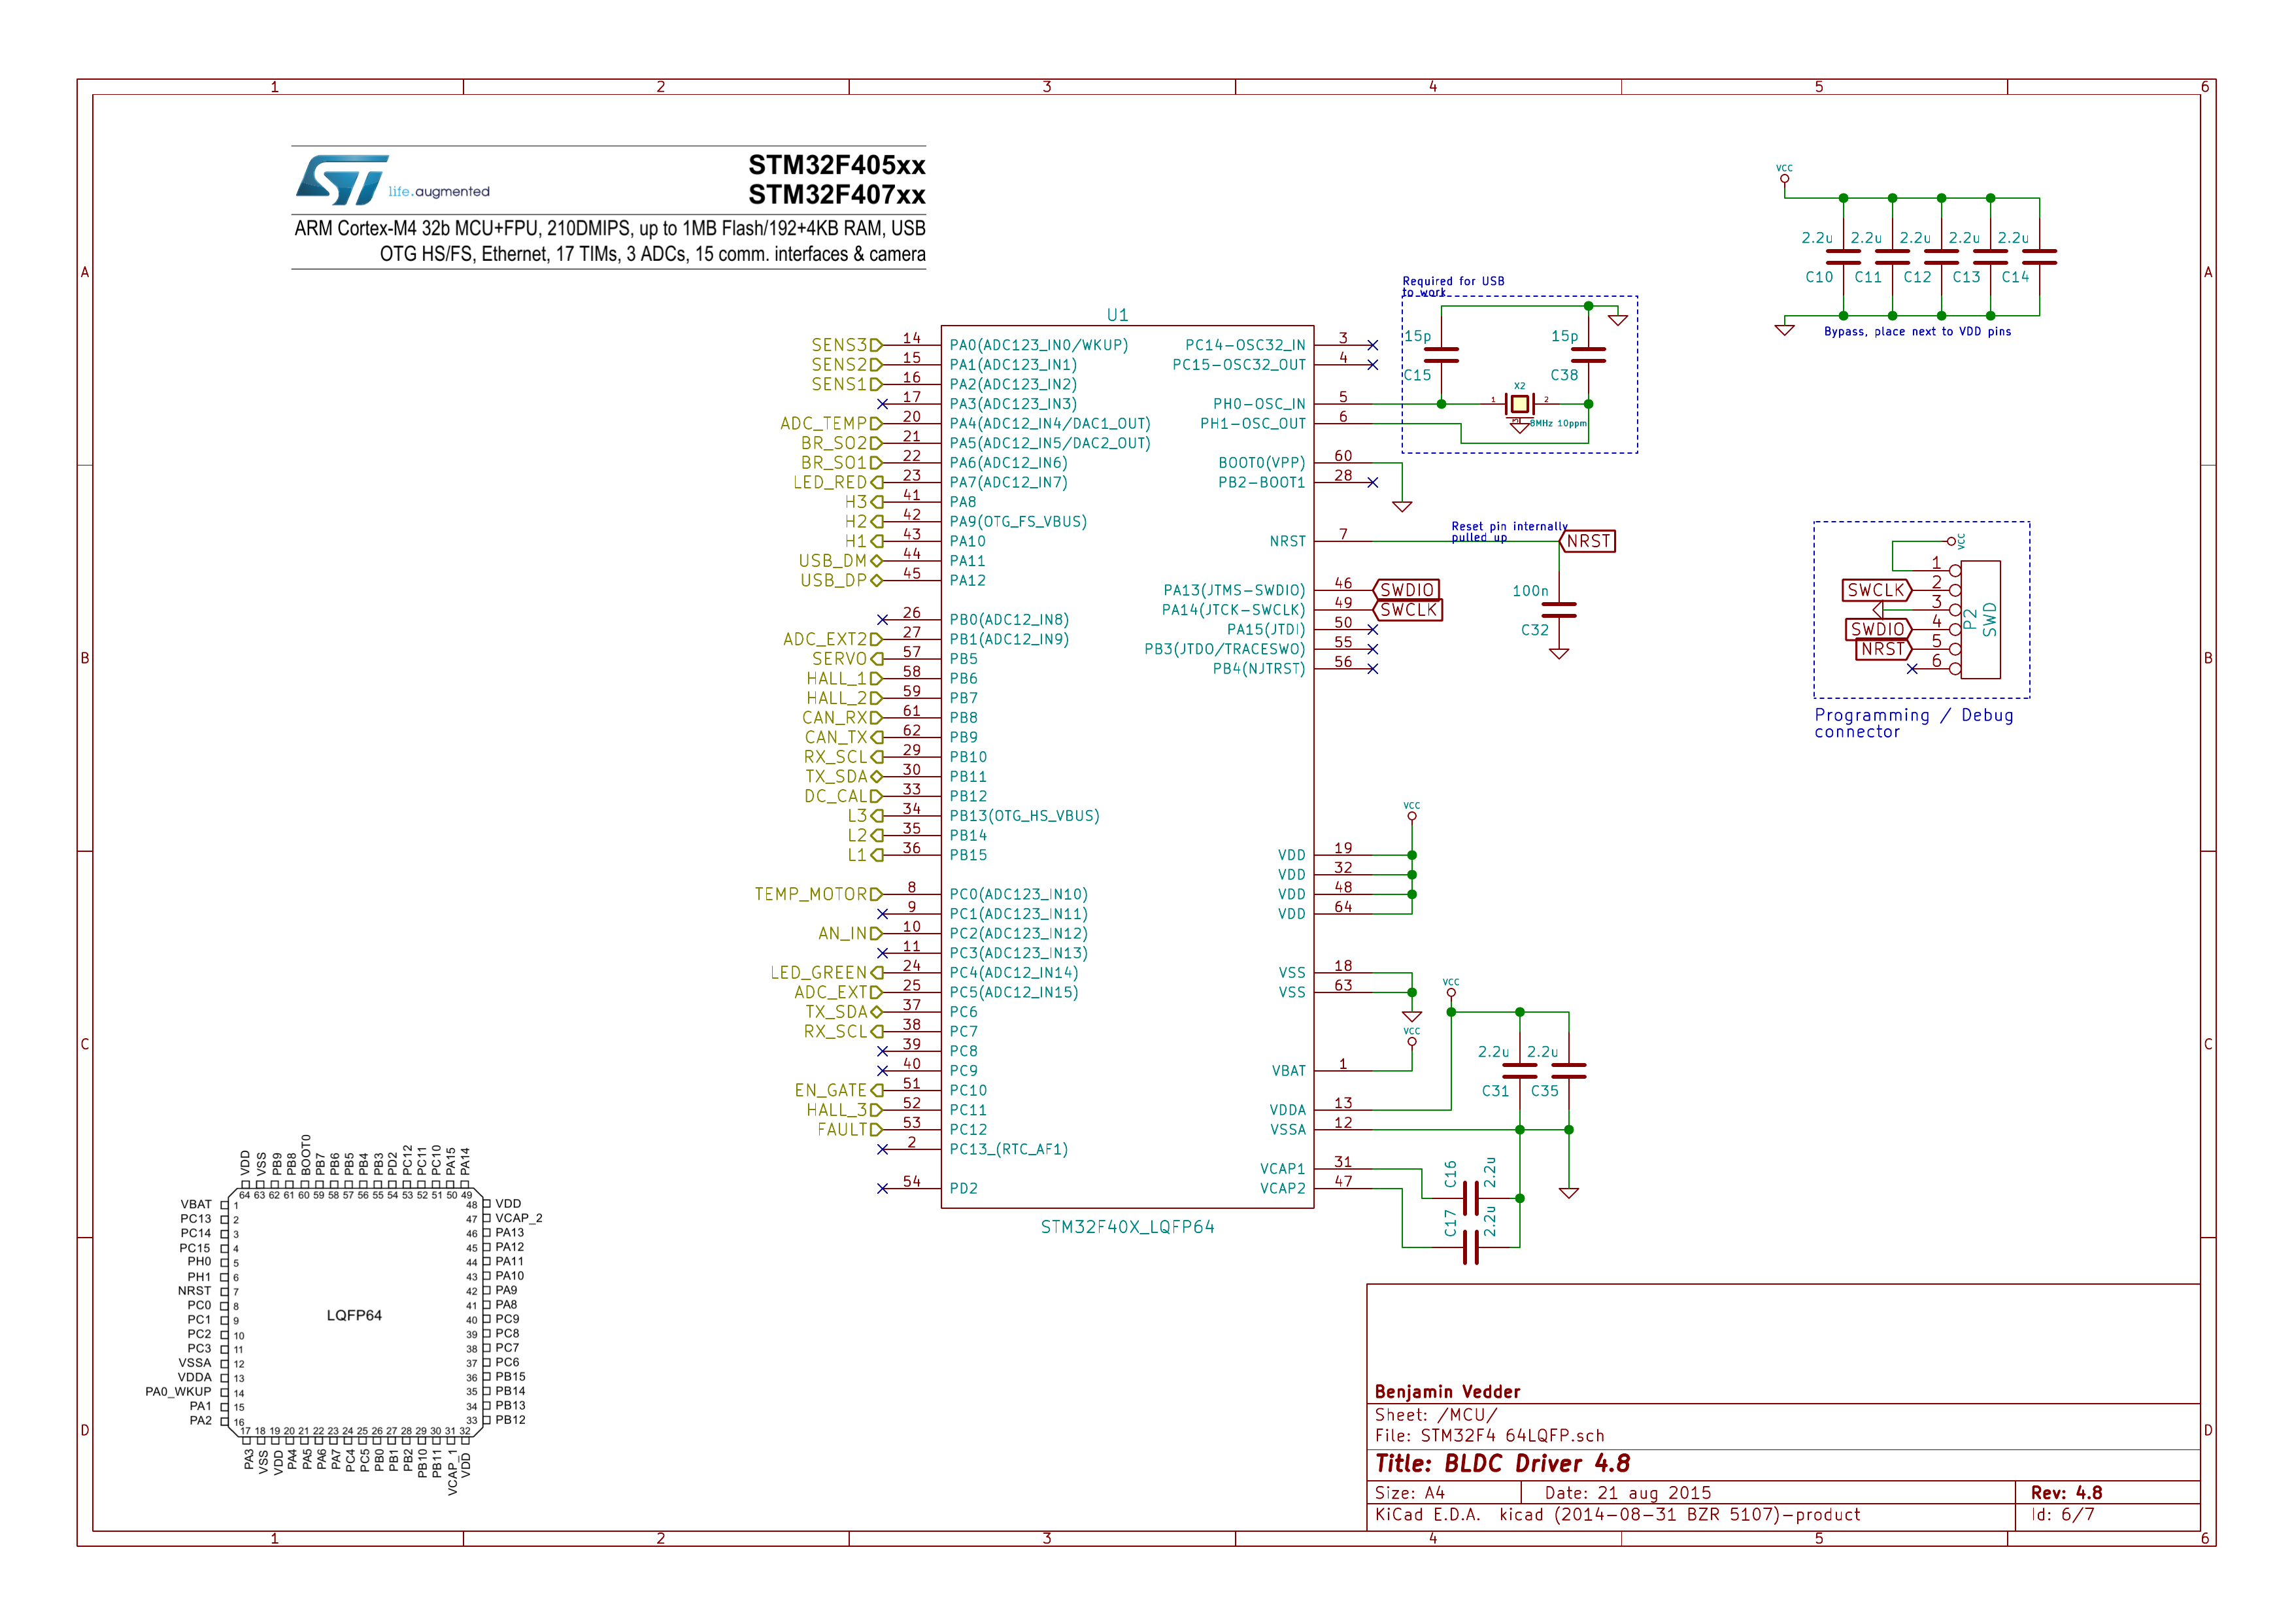
\includegraphics[width=\textwidth]{VESC/Schematic-6.png}
     
És un microcontrolador encarregat de controlar la major part del driver, des de les comunicacions fins al control de les oscil·lacions dels mosfets de potència. Per això disposarem de diversos comptadors, 17 de 15 de 16bits + 2 de 32 bits, per tal de generar les ones PWM o estar alerta en les comunicacions, entre altres funcions. Hi hauran diversos protocols de comunicacions tal com UART, I2C, CANBUS i SPI en un total de 15 ports, de forma que tindrem una gran capacitat d'adaptació a dispositius externs com comandaments o data-logers. A part disposem de dos Ethernet de 10/100 mbps per comunicacions avançades i usb, par tal de configurar-lo o capturar dades mitjançant computadors.\footnote{https://www.st.com/resource/en/datasheet/dm00037051.pdf}
     
\section{Algorismes de control}
Una vegada analitzat com està construït el controlador, anem a fer un repàs del codi del controlador. No serà un repàs exhaustiu del funcionament del firmware, però si poder veure una visió general de com funciona el control dels motors.
    
\subsection{Per què ens hem basat en el VESC}
És un dels pocs projectes d'aquest tipus que hi ha al mercat, però tot i així s'ha convertit en un referent i les marques privades l'utilitzen en els seus dispositius. A part poden analitzar el seu codi i entendre les funcions que fa per tractar d'implementar el nostre, modificar el VESC o decantar-no per utilitzar aquest controlador. A part he pogut analitzar una mica com està connectat i perquè està muntat com ho està, quins efectes apareixen al controlar motors en triple pont i que tenir en compte, coses que en l'electrònica explicada es tenien en compte ja que no tractàvem la potència.

\subsubsection{Efectes que apareixen el el pont en H}
En el control de motors de corrent continu els controlem amb el pont en H o el semipont en H. En aquest cas ens centrarem en el pont en H ja que és més similar al triple pont en H que és el que aplica el projecte.

\subsubsection{Pont en H en corrent continu}
En el moment que volem controlar un motor en els dos sentits controlant tant el corrent com el sentit d'aquest, és la selecció ideal.

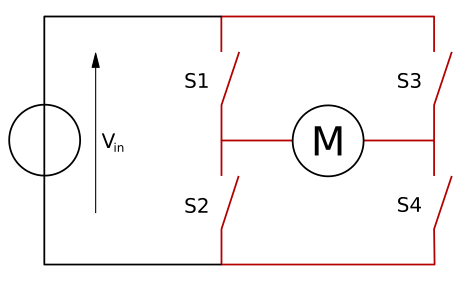
\includegraphics[width=\textwidth]{VESC/Hbritge.png}\bigskip
 
Depenent de la combinació de la commutació dels interruptors tenim diferents efectes. En el cas commutem S1 i S4 o S2 i S3 el motor girarà en un sentit o en l'altre, això provocarà que el corrent de la font vagi directament als pols del motor i provoqui la màxima potència en algun dels sentits. Si el control es realitza per pulsacions PWM podem controlar el corrent que li enviem al motor per tal de fer que funcioni a mig gas o com vulguem. 
 
S'ha de tenir en compte l'efecte que ha de deixar un motor girant amb el pols a l'aire, un motor girant és un generador de corrent, és a dir, que convertirà la seva energia cinètica en corrent que s'acumularà als pols del motor. Això pot provocar un pic de sobrecorrent en el transistor que controla el pont. S'han de muntar díodes de descàrrega en sentit oposat o mantenir els interruptors activats per tal de drenar el corrent generat pel motor.

Si en algun moment volem efectuar una parada ràpida del motor, podem jugar alimentant el motor en sentit contrari, en el cas que el control ho permeti, o podrem curtcircuitar els seus pols per tal de provocar un curtcircuit i fer desaccelerar el motor ràpidament. Això ho faríem activant S1 i S3 o S2 i S4 de forma que el corrent generat circuli per la part superior o inferior del pont.

\subsubsection{Rectificador trifàsic en CC}
El rectificador trifàsic és el mateix que el pont en H però afegint una branca més per poder treure les 3 fases.

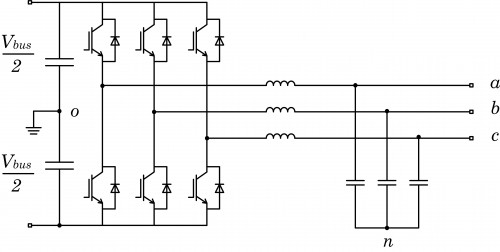
\includegraphics[width=\textwidth]{ilustracion-1-13281.jpg}\bigskip

Tenim el mateix que en el pont en H però amb una tercera branca. En el cas del rectificador trifàsic normalment es poden afegir uns filtres de corrent i voltatge a les bobines i codificar per tal d'estabilitzar l'ona generada ja que el control serà per polsos. Tant el voltatge com el corrent seran polsants, d'aquesta manera podríem filtrar harmònics que podrien ser no desitjats, depenent de com commutin S1, S2 i S3 (superiors) i S4, S5 i S6 (inferiors) podríem crear la forma d'ona i la freqüència desitjada per tal d'enviar-la al rectificador.
%tenim el matex que el pont en H per amb una tercera branca, en el cas del trectificafot trifaisc normalemnt es poden afagir un filtres de corrtent i volatrga, bobines i condececodr per tal de entabilisar la ona generada ja que el control sera per pulsos i tan el voltatge i el cotrent sera pulsat, de aquenta menre podriem filtrar armonics que podrien ser no desigats, depenent de com comuent s1 s2 s3 (superiors) i s4 s5 i s6 (inferiors) podriem crear la forma de ona i la frecuencida desitgada per tal de enviar al rectificador.\medskip

També cal tenir en compte que volem controlar motors brushless i el seu control és com el d'un motor CC, amb la diferència que tenen 3 fases i per tant els filtres no serien necessaris i podrien molestar ja que tot filtre provoca retards i no seria útil en el nostre cas.

\section{aspectes a teir en conte}
Una vegada repassat com funciona el control dels motors brushless per vehicles elèctrics ens adonem que en el control tenim molts aspectes que influeixen com pot ser la freqüència de commutació, la fase del motor, la freqüència de l'ona generada i la posició del roto, com plantegem cada una d'aquestes característiques i com les controlem.

\subsubsection{Freqüència de commutació}

Si podem controlar la freqüència de commutació dels transistors podrem millorar l'eficiència de l'inversor trifàsic, és a dir, a una menor freqüència les pèrdues de commutació seran menors i el corrent que li arribarà al motor tindrà un menor soroll. suposem que volem generar polso quadrats a una freqüenta de 1khz en el 80/100 del voltege per tal de controlar el motor, si el nostre pwm commuta a 500khz el que ens trobarem es que commutem moltíssimes vagades, axó provocarà sobreescalfament en el mosfets, ja que dissipen molta més potencia en commutació, i un soroll molt important en el motor, per tal si vexem la frecuancia de commutació a 100khz, podríem generar la mateixa ona però amb 400 comunicacions menos per segons el que milloraria la eficacia

% CURT? AQUI COMENTAM AVIAM SI AFEGIRAS MES O QUE FARAS, SINO POTSER FAIG UN APAÑO

\section{Selecció del control desitjat i modelació de la PCB}

Per tal de poder adaptar el nostre sistema al VESC necessitaríem fer unes millores en l'electrònica i una modificació del firmware per tal de suportar voltatges més alts deguts a la complicació que tenim a l'hora de controlar el ponts en H. Això és una feina que ja vam provar amb una complexitat molt elevada.

\input{Resultats/Resultats_Brunet}
\chapter{Motostudent}
\label{chap:motostudent}

El Motostudent és un projecte educatiu que tracta en dissenyar i construir una moto elèctrica. Un cop s'implementi la moto es realitzaran una sèrie de proves en el circuit de Motorland a Aragó. No és el mateix ordre de magnitud que un patinet elèctric pero ha sigut una gran experiència per veure els problemes i les solucions en els vehicles elèctrics.

En el tema de les bateries he pogut viure en primera tot lo fàcil que sembla al principi i lo complica que és a la realitat. El fet de dissenyar una bateria per una aplicació en concret, construir-la i mantenir-la amb sistemes de BMS ha suposat una millora dels meus coneixements en tot aquest camp. Hi ha molts aspectes a tenir en compte; les cel·les per fabricació no són idèntiques i això provoca que s'hagin de tenir en compte a l'hora de connectar-les ja que poden tenir diferències de voltatge que es dissipen en el moment de la connexió. S'han de pensar on i com es posen els termistors per veure les diferències de temperatura en la bateria, i com es refredarà en el cas que sigui necessari. També vaig veure la realització de les connexions per tal de que la intensitat quedés repartida en dos packs de cel·les, una de 24 cel·les i una altra de 4, formant la bateria total de 28. S'havia de tindre en compte que la intensitat havia de quedar dividida en paral·lel entre els dos packs i per tant calia repartir la intensitat de les 24 cel·les a aquestes 4 per tal de balancejar al complert la bateria. 
%en el tema de les baterias he pugut contatar lo facil que semble i lo complicat que es el fet de disnay una baterya per una aplicaico en concaret costryila i mentanirla amb sistemas de BMS, hi han tot de especters a tenir en conte, es a dir les celes per ontrucio no son identecac i axo proboca que agis de nar en conte a lora de connectarles ja que poden tenir petites difarencias de voltage que es disiparen el el moment de la connexio, san de pensar on i com es posen els termitors per veure las difarencias de temperatura en la bateria, i com es refarada en el cas que sigui nesesari, com es realisaren les connexions per tal de que la intenciat en dividexon en el paralel en cuestrio, es d dir la bateria no eran 28 celens en seria sino que tambe en tenin 4 en paralel i axo probocaba que sagen de repartit la intenciat totl en aquets 4.\smallskip

He pogut veure els riscs que comporta treballar amb bateries d'alt voltatge, ja que no disposen de cap sistema de protecció per tal de tallar la potència quan s'estiguin manipulant. En una empresa per exemple, si es produeix un curtcircuit existeixen mesures de protecció com per exemple magnetotèrmics diferencials que evitant que algú es pugui quedar enganxat al corrent. Al treballar amb bateries no es van tenir cap d'aquests sistemes de control per tant es van haver d'aplicar unes grans mesures de protecció i anar amb molt de compte al manipular-les. 

També he pogut veure els sistemes d'activació de la potència. En el cas de la bicicleta no s'han tingut en compte ja que el voltatge i la potència són relativament baixos. En la moto es disposava d'un sistema que determinava si connectava o no la bateria a la resta de la moto o si permetia els pas de corrent del carregador a la bateria. Aquest sistema de control activava el controlador del motor, el qual li subministrava la potència a ell i el BMS controlava el carregador, de forma que abans de permetre el pas de potència comprovaven l'estat de la bateria.
%sitemas de activacio de la potencia, en el cas del patinet no san tingut en conte ja que el voltage i la potencia son reletivament baixes pero en la moto disposava de un sistema que daterminava si connectava o no la baterya al resto de la moto o si permetia el pas de corrent del carregador a ala baterya, aquets sistemas de contorl anava activar el el controlador de motor el que li sumnistrava la potencia a ell i el bms controlaba el caregador, de forma que avans de permentre el pas de potencia comprovaven el estat de la baterya.\smallskip 

Per controlar la moto es va anar per un model de convertidor comercial, un controlador per a motors brushless ja que les potències podien arribar als 48KW. Això requeria d'una electrònica i control molt estable. El control havia d'estar alimentat per dues fonts separades; una que era la bateria principal i l'altre la bateria de control, la qual només activava els sistemes de càlcul del BMS i el Driver per tal de determinar si estava o no estava a punt per controlar el motor.

En el control de la bateria vam optar per un orionBMS que és un model comercial de BMS el qual ens permet controlar l'anivellació de les cel·les i el seu voltatge i intensitat que es drena de la bateria. A part de disposar de dues interfícies de communicació canbus per tal de controlar el carregador de bateries i treure informació.

%ziban??????
El carregador era en ziban el qual podia injectar fins a 50A a la bateria, els seus paràmetres d'intensitat, voltatge i ones de càrrega anaven controlats per una interfície canbus, en el qual el BMS i el carregador s'havien d'entendre i demanar els paràmetres òptims per a la càrrega.
%el carragador era en ziban el cual podei ingectar fins a 50A a la beterya, els seus paremntres de intenciat voltage i odes de carrega anavan controlats per un inteface canbus, en el cual el bms i el caragador savien de entendre i demanr els paramentes optims per a la carrega\smallskip

El blender era un sistema que es dedicava a la vigilància de que les fonts de voltatge LOW i HIGH no estiguessin connectades per tallar la bateria en cas que passés. És un sistema de seguretat que es basa en que el sistema de potència sigui un sistema totalment aïllat tant en el positiu com en el negatiu, i que no tingui sortida en cap massa.

Un cop obtinguts tots els resultats ens vam reunir tot l'equip i vam fer una pluja dels problemes i aspectes a corregir sobre la moto. És allà on hem vaig adonar de la dificultat del projecte que estàvem portant entre mans. Durant el període del disseny vam estar cuidant tots els elements per a garantir una moto de qualitat. En aquell moment semblava que tot anava sobre rodes, però després al dia d'avui m'adono que vam passar per alts petits detalls que al final van portar molts mal de caps. Aspectes que no vam tenim en compte com el soroll emès per un corrent de 500A a 110V passat per cables no apantallats, fent inservible l'electrònica. El BMS no detectava els voltatges de les cel·les i tallava la bateria, ja que saltaven els sistemes de seguretat només pel soroll emès. En futures millores realitzarem tot el cablejat apantallat i controlarem la direcció i els retorns dels camps per tal d'anular al màxim aquests efectes. El sistema d'aïllament ens tallava la bateria en el procés de càrrega ja que, el canbus del carregador es connectava amb el canbus de la moto, on l'aïllament no era suficientment alt. Per això es va haver de puntejar el sistema d'aïllament per poder carregar la moto.

Les comunicacions eren inútils en el moment de càrrega o descàrrega de la bateria ja que el soroll provocat i el no anar amb cables apantallats ni trenats provocava errors a les comunicacions.

Trobo que ha estat una experiència molt educativa, molt bona en tots els sentits, pero trobo que la nostra universitat no ho té en compte, i es fan petites activitats com el futbol. És un projecte on s'aprén com funcionen les coses i com la teoria no quadra per als petits detalls.


\chapter{Conclusions}
\label{chap:conclusions}

Després de la realització del projecte i amb tot l'estudi previ que hem realitzat em trobo en posició de determinar que no era conscient de la complexitat que suposa controlar el voltatge i la quantitat de paràmetres que s'han de tenir en compte per tal de controlar aquestes magnituds. Per tant l'abast del projecte inicial ha estat reduït ja que tenia al cap el disseny com la construcció d'un controlador de vehicles elèctrics. Encara hi han aspectes de l'electrònica de potència que no he assimilat completament i no podria dissenyar un controlador estable sense ajuda. He pogut aprofundir en el control de motors i els tipus de controls que existeixen, en el món dels vehicles elèctrics i cap on va el món del petit VE.

A l'acabar el projecte col·laborant amb MotoStudent veig que la complicació també la tindrem de punts que no he tingut en compte com les emissions dels cables de potència i la seguretat en sistemes de protecció de les bateries, és a dir, mantenir els circuits aïllats i amb el control de les emissions per tal de no espatllar les mesures. Així que em queda seguir treballant per entendre els motors elèctrics per poder-me dissenyar un petit vehicle elèctric.


\end{document}